%==================================================================================================
%   LUKES THESIS TEMPLATE 1.2
%   -------------------------
%   This template is based upon the offcial IMM PhD Thesis template, it is enhanced with a number
%   of new features and a number of errors have fixed. This template is intended to be complied to
%   PDF using PDFLATEX and is tested using the MiKTeX 2.9 LaTeX distribution.
%   It is based on the official DTU-IMM Thesis template by Finn Kuno Christensen in 2009.
%   Small bugfixes by Kasper Laursen in 2012.
%   -------------------------
%   Last Updated: 2012-09-19
%   Contact: lthhe@imm.dtu.dk
%
%	Edited by Emilio Potenza & Marco Galardini
%==================================================================================================
%
%==================================================================================================
% DOCUMENT SETUP
%==================================================================================================
\documentclass[12pt,twoside]{book}                  %Official DTU-IMM Thesis document setup
%
%Set to 'print' for printed version, use 'net' for online version
\def\thesisversion{print}
%
%==================================================================================================
% PACKAGES
%==================================================================================================
\usepackage{LukeThesis}                             %Import Thesis base style
%input{PhDMacros}
\usepackage[width=15pt, height=auto, eventxtindent=2pt, oddtxtexdent=2pt]{thumbs}							   %Macros for thumb-index

\newcommand{\newthumb}{\addthumb{Section \thechapter}{\thechapter}{black}{gray}}
\newcommand{\myparagraph}[1]{\paragraph{#1}\mbox{}\vspace{10pt}\\}                                   %Thesis specific macros

%
%==================================================================================================
% MANUAL EMILIO, GALA & GIOVANNI :)
%==================================================================================================
\usepackage{mathptmx}
\usepackage{svg}
\linespread{1.15}


%
%==================================================================================================
% THESIS PROPERTIES (Modifiy these fields with your details)
%==================================================================================================
\def\thesisauthor{Giovanni Bacci}                     %Author
\def\thesistitle{}  %Title
\def\thesishandin{31 December}                       %Submission date (Day-Month}
\def\thesisdegree{PhD}                              %Degree ('B.Eng', 'B.Sc.', 'M.Sc.' or 'PhD')
\def\thesisyear{2014}                               %Submission year
\def\thesisnumber{1}                             %DTU-IMM Serial number (do not include year
\def\thesisISSN{1}                          %ISSN number

\def\thesiskeywords{}  %PDF keywords
\derivethesisprops                                  %Derive dependent properties
%
%==================================================================================================
% SECTION NUMBERING SETUP
%==================================================================================================
\setcounter{tocdepth}{3}                            %2 adds sections up to subsections
\setcounter{secnumdepth}{3}                         %Subsubsections get a number when this is 3
%
%==================================================================================================
% THESIS STRUCTURE  (Modifiy to include more chapters etc)
%==================================================================================================
\begin{document}
%------------------------
%Pre-frontmatter material
%------------------------

\prefrontmatter

\normalsize
%--------------------
%Frontmatter material
%--------------------
\frontmatter
\pagenumbering{roman}                               %Set frontmatter numbering style


%*******************************************************
% Acknowledgments
%*******************************************************
\pdfbookmark[1]{Quotes}{quotes}

\thispagestyle{empty}

\begin{flushright}{\slshape
	\textit{By striving to do the impossible, man has always achieved what is possible. Those who have cautiously done no more than they believed possible have never taken a single step forward} \\
	Mikhail A. Bakunin\\*[0.5cm]
	\textit{It is only those who do nothing who makes no mistake} \\
	Pyotr Kropotkin\\*[0.5cm]
	\textit{A man provided with paper, pencil, and rubber, and subject to strict discipline, is in effect a universal machine} \\
	Alan Turing\\*[0.5cm]
	\textit{Don't try to solve serious matters in the middle of the night} \\
	Philip K. Dick\\	
	}
\end{flushright}



\newpage

\begingroup
\let\clearpage\relax
\let\cleardoublepage\relax
\let\cleardoublepage\relax

\chapter{Acknowledgements}

{\small
First of all I would like to thank my supervisors: Professor \textbf{Alessio Mengoni} and Doctor \textbf{Anna Benedetti} for their constant presence and contagious enthusiasm.

\noindent I also would like to thank the COMBO (Florence computational biology group) in the persons of \textbf{Marco Galardini}, \textbf{Marco Fondi} and \textbf{Emanuele Bosi} for their advices and all discussions made in front of an old whiteboard.

\noindent Special thanks to Professor \textbf{Marco Bazzicalupo} and Professor \textbf{Alberto Ugolini} for gave me the opportunity to join in their research activities.

\noindent Many thanks to \textbf{Francesco Vitali} for sharing with me the experience of a PhD in the Department of Biology of the Florence University.

\noindent Thanks to all of those who have gravitated around the Specola and Sesto Fiorentino during these years, and especially \textbf{Alice Checcucci}, \textbf{Isabel Maida}, \textbf{Elena Perrin}, \textbf{Angela Frascella}, \textbf{Giulia Spini} and \textbf{Amaranta Focardi} for all the good laughs.

\noindent Many thanks to my family which has always supported me in all these long years of neverending studies: I wouldn't have made it without your presence.

\noindent Last but not least, thanks to \textbf{Adele Giannetti} for standing by me every time I was not-so-enthusiastic about what was going on.
}

\endgroup



                            %Acknowledgements
\markboth{}{}                                       %Set headings (left)(right)

%*******************************************************
% Publications
%*******************************************************
\pdfbookmark[2]{Publications}{publications}

\chapter{Publications list}

Most of the data presented in this thesis has been published in the following \textit{peer-reviewed} papers:
\begin{itemize}

\item \textbf{Bacci, G.}, Bazzicalupo, M., Benedetti, A., \& Mengoni, A. (2014). StreamingTrim 1.0: a Java software for dynamic trimming of 16S rRNA sequence data from metagenetic studies. \textit{Molecular ecology resources}, 14(2), 426-434.

\item Mengoni, A., Focardi, A., \textbf{Bacci, G.}, \& Ugolini, A. (2013). High genetic diversity and variability of bacterial communities associated with the sandhopper \textit{Talitrus saltator} (Montagu)(Crustacea, Amphipoda). \textit{Estuarine, Coastal and Shelf Science}, 131, 75-82.

\item \textbf{Bacci, G.}, Pagoto, E., Passaponti, M., Vannocci, P., Ugolini, A., \& Mengoni, A. (2014). Composition of supralittoral sediments bacterial communities in a Mediterranean island. \textit{Annals of Microbiology}, 1-13.

\item Borruso, L., \textbf{Bacci, G.}, Mengoni, A., De Philippis, R., \& Brusetti, L. (2014). Rhizosphere effect and salinity competing to shape microbial communities in \textit{Phragmites australis} (Cav.) Trin. ex-Steud. \textit{FEMS microbiology letters}, 359(2), 193-200.

\item Bevivino, A., Paganin, P., \textbf{Bacci, G.}, Florio, A., Pellicer, M. S., Papaleo, M. C., ... \& Dalmastri, C. (2014). Soil Bacterial Community Response to Differences in Agricultural Management along with Seasonal Changes in a Mediterranean Region. \textit{PloS one}, 9(8), e105515.

\item Canfora, L., \textbf{Bacci, G.}, Pinzari, F., Papa, G. L., Dazzi, C., \& Benedetti, A. (2014). Salinity and bacterial diversity: to what extent does the concentration of salt affect the bacterial community in a saline soil?. \textit{PloS one}, 9(9), e106662.

\item \textbf{Bacci, G.}, Bani, A., Bazzicalupo, M., Ceccherini, M.T., Galardini, M., Nannipieri, P., Pietramellara, G., \& Mengoni, A. (2015). Evaluation of the performances of Ribosomal Database Project (RDP) Classifier for taxonomic assignment of 16S rRNA metabarcoding sequences generated from Illumina-Solexa NGS. \textit{Journal of Genomics}, 3, 36-39.

\item \textbf{Bacci, G.}, Ceccherini, M.T., Bani, A., Bazzicalupo, M., Castaldini, M., Galardini, M., Giovannetti, L., Mocali, S., Pastorelli, R., Pantani, O.L., Arfaioli, P., Pietramellara, G., Viti, C., Nannipieri, P., \& Mengoni, A. Exploring the dynamics of bacterial community composition in soil: the pan-bacteriome approach. Manuscripts in press in: \textit{Antonie van Leeuwenhoek}.

\end{itemize}

% Book chapter
\noindent \textit{Book chapter}
\begin{itemize}

\item \textbf{Bacci, G.} (2015). Raw Sequence Data and Quality Control. In \textit{Bacterial Pangenomics} (pp. 137-149). Springer New York.

\end{itemize}


% Submitted for publication
\noindent \textit{Submitted for publication}

\begin{itemize}

\item \textbf{Bacci, G.}, Abdelrhman, K.F.A., Marras, B., Nistri, A., Schintu, M., Ugolini, A., \& Mengoni, A. The gut microbiota of talitrid amphipods provides insight into the ecology of supralittoral sediments detritivors. Manuscripts submitted to: \textit{FEMS Microbiology Ecology}.

\item Paganin, P., Fiscarelli, E.V., Tuccio, V., Chiancianesi, M., \textbf{Bacci, G.}, Morelli, P., Dolce, D., Dalmastri, C., De Alessandri, A., Lucidi, V., Taccetti, G., Mengoni, A., \& Bevivino, A. Changes in Cystic Fibrosis Airway Microbial Community Associated with a Severe Decline in Lung Function. Manuscripts submitted to: \textit{PloS one}.

\item Galardini, M., Spini, G., Rossi, M., Roncaglia, B., Bani, A., \textbf{Bacci, G.}, Pini, F., Brilli, M., Biondi, E.G., Bazzicalupo, M., \& Mengoni, A. Evolution of intra-specific regulatory networks in \textit{Sinorhizobium meliloti}. Manuscripts submitted to: \textit{PLOS Computational Biology}

\end{itemize}


% Other articles in preparation related to this thesis
\textit{In preparation}

\begin{itemize}

%\item Di Carli M., De Rossi P., Paganin P., Del Fiore A., Lecce F., Capodicasa C., Bianco L., Perrotta G., Mengoni A., \textbf{Bacci, G.}, Benvenuto E., Vitali F., Daroda L., Dalmastri C., Donini M., Bevivino A. Bacterial community composition and proteome content of fresh-cut lettuce as affected by packaging.

\item \textbf{Bacci, G.}, Paganin, P., Lopez, L., Vanni, C., Dalmastri, C., Cantale, C., Daddiego, L., Perrotta, G., Taccetti, G., De Alessandri, A., Fiscarelli, E.E., Lucidi, V., Bevivino, A., \& Mengoni, A. Taxonomic signatures of CF airway microbiota distinguish between stable and severe declining patients. Manuscripts to be  submitted to: \textit{Proceedings of the National Academy of Sciences}


\end{itemize}


% Conference papers
\textit{Conference papers}

\begin{itemize}

\item \textbf{Bacci, G.} (2012, June). \textit{Elementi di Bioinformatica}. Paper presented at Scuola di Biodiversità e Bioindicazione della Società Italiana Scienza del Suolo. Rome, Italy.

\item \textbf{Bacci, G.}, Bazzicalupo, M., Benedetti, A., \& Mengoni, A. (2013, October). \textit{StreamingTrim 1.0: a Java software for dynamic trimming of 16S rRNA sequence data from metagenetic studies}. Paper presented at Bioinformatiha 2. Florence, Italy.

\item \textbf{Bacci, G.}, Bazzicalupo, M., Benedetti, A., \& Mengoni, A. (2013, December). \textit{StreamingTrim 1.0: a Java software for dynamic trimming of 16S rRNA sequence data from metagenetic studies}. Poster presented at 2\textsuperscript{nd} T\"{u}nen symposium on soil Metagenomics: mining and learning from metagenomes. Braunschweig, Germany.

\item Canfora, L., \textbf{Bacci, G.}, Pinzari, F., Papa, G. L., Dazzi, C., \& Benedetti, A. (2013, December). \textit{Metagenomic approach applied to the microbial community of a saline soil with high spatial variability}. Poster presented at 2\textsuperscript{nd} T\"{u}nen symposium on soil Metagenomics: mining and learning from metagenomes. Braunschweig, Germany.

\item \textbf{Bacci, G.} (2014, May). \textit{Inspecting the dynamics of bacterial communities. The pan-bacteriome approach}. Paper presented at Cortona Procarioti. Cortona, Italy.

\item \textbf{Bacci, G.}, Bazzicalupo, M., Benedetti, A., \& Mengoni, A. (2014, May). \textit{StreamingTrim 1.0: a Java software for dynamic trimming of 16S rRNA sequence data from metagenetic studies}. Paper presented at PhD Day\textsuperscript{5}. Sesto Fiorentino, Italy.

\end{itemize}

%The source files of this thesis will be available after the discussion as a git repository on \href{https://github.com/mgalardini/PhDGala}{GitHub} (@mgalardini).
									%Publication list
\markboth{}{}

%*******************************************************
% Abstract
%*******************************************************
\pdfbookmark[3]{Abstract}{abstract}
\chapter{Abstract}
Bacteria are everywhere and they make up for their microscopic dimension in sheer number. Thanks to their great functional and taxonomic variability, bacteria plays a pivotal role in several environments. In soil they are responsible for some of the most important biogeochemical cycles and for the cycling of organic compounds. They reside even on both the surface and in deep layers of human skin, in the saliva and oral mucosa, in the conjunctiva, and in the gastrointestinal tracts performing tasks that can be useful for the human host. They were able to colonize extreme environments and, thanks to their ability to break down hazardous substances into less toxic or non toxic substances, they are used as bioremediation agents for removing pollutant from contaminated sites. Nevertheless, the study of microbial diversity patterns is still hampered by the enormous diversity of microbial communities and the lack of resources to sample them exhaustively.\\
Difficulties in bacterial cultivation and isolation are even today one of the main obstacle for the correct identification of both bacterial taxonomies and bacterial functions. A range of novel methods, most of which are based on rRNA and rDNA analyses, have uncovered part of the microbial diversity in several environments but the percentage of characterized organisms remains low (approximately 1-5\% of the whole bacterial biodiversity). The next step in the ``genomic era'' is to extract genomic, taxonomic and functional informations directly from bacterial communities genome (the metagenome). This concept moved our perspective of bacterial diversity to a ``meta'' point of view. To this end, the advent of the Next Generation Sequencing (NGS) techniques has made it technically possible to exhaustively sequence entire bacterial communities without the need to isolate single strains. Therefore, developing new methods and protocols for studying bacterial patterns in different environments is becoming one of the most competitive challenge to date.\\
The work here presented is part of this perspective and it can be easily divided into three different major parts: the first (named ``Small tools for big data") deals with all issues related to processing and exploitation of sequence data in a metagenomic analysis. In particular, performing this kind of analysis require generating a huge amount of data which can't be easily managed even by most sophisticated computers. For this reason is crucial developing bioinformatic algorithms able to handle a big number of sequences with a small amount of memory and processor resources. Results obtained within this part of the work have underlined the need both to improve available tools and to develop new software for analysing metagenomic data. Specifically, one of the most used tool for taxonomic classification of rRNA sequences from metabarcoding analyses was benchmarked: the ``Ribosomal Database Project'' Classifier (RDP Classifier). This analysis has shown a decreasing level of resolution passing from Phylum to Genus level highlighting the need of continuous improvements in current classification algorithms. On the other hand, a new tool for quality refinement of metagenomic data has been developed. This tool is able to remove low quality segments from raw sequence data retaining as much information as possible. Furthermore, the amount of memory required for this tool to work is proportional to the length of the sequence analysed and it is not related to the number of sequences to analyse, making this tool very useful for metagenomics analyses.\\
The second part of this work includes three different chapters named: ``Bacteria-environment interaction'', ``A life in transition: bacteria in harsh environments'' and ``Bacteria in agro-environments''. Basically, this part covers both functional and taxonomic classification of bacteria in different environments. In particular, changes in bacterial community composition have been inspected from three different perspectives: natural environments, extreme environments and agricultural environments. In all these ambiances, bacteria were found capable of shaping their composition based on either external perturbing agents (entropic gradient, salinity, pollution...) or time. Developing methods for studying bacterial community is one of the crucial tasks in metagenomics where even obtain an overview of bacterial community data could be a very difficult task (especially in complex environment like soil).\\
In the last part of my work, bacterial communities have been analysed as both human and animal hosts. From the animal side, the gut microbiota of talitrid amphipods has been analysed in order to inspect changes in bacterial communities related to different species and locations. Results obtained have shown that is possible to generate a bacterial fingerprint for both inspected factors, underlining that, either different species or different diets are able to influence bacterial gut composition. From the human side, the composition of bacterial communities has been inspected in patients with a specific pathological conditions: cystic fibrosis. Understanding differences in bacterial populations related to this pathological state is very important for either developing new treatments or improving existing ones. In addition, reported results highlight the importance of microbiome inspection for the selection of bacterial groups that may be related to the uprising of a particular human disease.\\                                   %English summary of Thesis
\markboth{}{}                                       %Set headings (left)(right)

%%*******************************************************
% Sommario
%*******************************************************
\pdfbookmark[4]{Sommario}{sommario}
\chapter{Sommario}
\begin{otherlanguage}{italian}

I batteri sono capaci di colonizzare quasi tutti gli ambienti presenti sul pianeta terra. Infatti, grazie alla loro plasticità funzionale e tassonomica, sono giocano un roulo importante in molti ambienti diversi. Nel suolo sono tra i principali responsabili del ciclo dei compositi organici ed altri importanti cicli biogeochimici ma riescono anche a vivere all'interno di organismi più grandi come ad esempio l'uomo. Infatti intere comunità batteriche sono state caratterizzare in diversi distretti del corpo umano come: sulla pelle, nella saliva, nella mucosa orale, nella congiuntiva e nel tratto gastrointestinale svolgendo funzioni essenziali per lo sviluppo dell'ospite. La loro plasticità li rende in grado di crescere e colonizzare anche gli ambienti più estremi e, grazie alla loro capacità di trasformare sostanze pericolose in sostanze poco (o per niente) tossiche, sono spesso utilizzati come agenti per la bonifica di aree inquinate. Purtroppo però lo studio delle popolazioni microbiche rimane difficoltoso sia a causa della loro grande variabilità genomica che per la mancanza di metodi per campionare esaustivamente complesse popolazioni.\\
Uno dei maggiori ostacoli all'identificazione di specie batteriche è la coltivazione e l'isolamento delle specie di interesse in condizioni di laboratorio. Infatti è stimato che solo l'1\% dei batteri sia in grado di essere coltivato e studiato usando metodi microbioloigici standard. Metodi di analisi innovativi, la maggiorn parte dei quali basati sull'analisi della sequenza del DNA ribosomiale, hanno permesso di scoprire nuove specie e funzioni batteriche ma la percentuale dei microorganismi caratterizzati rimane bassa (circa 1-5\% della biodiversità batterca totale). Il prossimo passo nell'era genomica sarà l'estrazione delle informazioni tassonomiche e funzionali direttamente dal genoma delle comunità batteriche (il cosiddetto ``metagenoma''). Questa sfida sta spostando la concezione della diversità batterica verso una prospettiva ``meta'' cioè un aprospettiva in grado di ``trascendere'' la definizione tradizionale di specie. Infatti, l'avvento delle tecniche di sequenziamento di nuova generazione (NGS) ha reso tecnicamente possibile il sequenziamento di intere comunità batteriche senza il bisogno di isolare singole specie rendendo lo sviluppo di nuovi metodi e protocolli per lo studio dei pattern batterici in ambienti diversi come una delle sfide più difficili e competitive dei nostri tempi.\\
Il lavoro qui presentato si inserisce in questo contesto e può essere concettualmente diviso in tre grandi aree tematiche. La prima area (comprendete il capitolo chiamato ``Small tools for big data'')  affronta i problemi legati al pre-processamento delle sequenze metagenomiche grezze e all'analisi finale delle sequenze ottenute. Infatti, affrontare uno studio metagenomico richiede solitamente la produzione di un elevato numero di sequenze rendendo questo tipo di analisi molto impegnativo da un punto di vista computazionale. Per questa ragione, la produzione di algoritmi bioinformatici in grado di analizzare grandi quantità di dati con una piccola quantità di risorse informatiche, sta divenatndo fondamentale per l'analisi di dati metagenomici. I risultati ottenuti in questa parte del lavoro sottolineano questa necessità. In particolare, le performace di uno degli strumenti più usati per la classificazione tassonomica delle sequenze di DNA batterico codificanti le subunità ribosomiali (il ``Ribosomal Database Project'' Classifier) sono state analizzate. Questa analisi ha mostrato una diminuzione del grado di risoluzione dell'algoritmo, passando dal livello tassonomica di Phylum a quello di Genere; ponendo l'accento sulla necessità di sviluppare algoritmi nuovi e più affidabili appositamente designati per analisi ``meta''. Per venire in contro a questa necessità, è stato sviluppato un nuovo software bioinformatico in grado di processare le sequenze metagenomiche grezze. Questo tool consente di rimuovere le regioni a bassa qualità da un set di sequenze metagenomiche, riducendò al minimo la quantità di dati persi. In aggiunta, il software in questione riesce a rifinire un grande numero di sequence in modo seriale, utilizzando quindi una piccola quantità di memoria dipendente unicamente dalla lunghezza delle sequenze e non dal loro numero rendendolo particolarmente adatto ad analisi metagenomiche.\\
La seconda parte di questo lavoro è composta da tre capitoli chiamati: ``Bacteria-environment interaction'', ``A life in transition: bacteria in harsh environments'' e ``Bacteria in agro-environments''. In questa parte sono stati discussi sia aspetti tassonomici che funzionali di comunità batteriche in ambienti naturali diversi. Cambiamenti nella composizione delle comunità batteriche sono stati analizzati in tre tipologie di ambienti: ambienti naturali, ambienti estremi e ambienti agricoli. In tutte le tipologie ambientali studiate, le comunità batteriche sono risultate essere capaci di modificare la loro struttura sia in risposta ad agenti perturbanti (gradiente antropico, salinità, inquinamento...) sia nel tempo. Lo sviluppo e la messa a punto di metodiche per lo studio di comunità batteriche complesse (come ad esempio nel suolo) sta diventando una tappa forzata per l'analisi di dati metagenomici dove anche semplicemente ottenere una visione di insieme della comunità in studio può essere motlo difficoltoso.\\
Nell'unlitma parte del mio lavoro, è stato investigato il ruolo di consorzi batterici come ``ospiti'' di organismi pluricellulari, in particolare l'uomo ed alcuni animali. Dal lato animale, il micorbiota intestinale di talitridi (\textit{Amphipoda}) è stato confrontato sia in specie diverse che in individui della stessa specie provenienti da aree geografiche differenti. I risultati ottenuti hanno mostrato che le comunità intestinali di questi animali sono molto diversificate e sembrano essere dipendenti sia dalla dieta (a sua volta legata dall'area geografica in studio) sia dalla specie. Sul lato umano invece, la composizione del microbiota è stata analizzata in pazienti affetti da una precisa patologia: la fibrosi cistica. In patologie strettamente legate ad infezioni poli-microbiche (come la fibrosi cistica) è molto importante capire a fondo le dinamiche che intrcorrono all'interno delle comunità batteriche in modo da sviluppare nuove cure o per migliorare quelle esistenti. In aggiunta, i risultati riportati mostrano che la selezione particolari firme tassonomicghe all'interno delle popolazioni batteriche umane può essere legato all'insorgenza o meno di particolari stai infettivi (peggioramento delle condizioni dei pazienti affetti dalla patologia).

\end{otherlanguage}                                   %Italian summary of Thesis
%\markboth{}{}                                       %Set headings (left)(right)


%------------------
% Table of contents
%------------------

\newpage\mbox{}\newpage
\chaptermark{Contents}
\pdfbookmark{\contentsname}{toc}
\renewcommand{\sectionmark}[1]{\markright{#1}}
\sectionmark{Contents}
\addtolength{\parskip}{-\baselineskip}
\tableofcontents
\addtolength{\parskip}{\baselineskip}
\renewcommand{\sectionmark}[1]{\markright{\thesection\ #1}}

%------------------
% List of figures
%------------------

\newpage\mbox{}\newpage
\chaptermark{Figures list}
\pdfbookmark{Figures list}{toc}
\renewcommand{\sectionmark}[1]{\markright{#1}}
\sectionmark{Figures list}
\addtolength{\parskip}{-\baselineskip}
\listoffigures
\addtolength{\parskip}{\baselineskip}
\renewcommand{\sectionmark}[1]{\markright{\thesection\ #1}}

%------------------
% List of figures
%------------------

\newpage\mbox{}\newpage
\chaptermark{Tables list}
\pdfbookmark{Tables list}{toc}
\renewcommand{\sectionmark}[1]{\markright{#1}}
\sectionmark{Tables list}
\addtolength{\parskip}{-\baselineskip}
\listoftables
\addtolength{\parskip}{\baselineskip}
\renewcommand{\sectionmark}[1]{\markright{\thesection\ #1}}

%-------------
% Main content
%-------------

\mainmatter
\part{Introduction}
\newthumb
%%%%%%%%%%%%%%%%%%%%%%%%%%%%%%%%%%%%%%%%%%%%%%
\logvartrue
\chapter{Background}
%%%%%%%%%%%%%%%%%%%%%%%%%%%%%%%%%%%%%%%%%%%%%%

Bacteria are often cited as examples of one of the Earth's most primitive living forms. Unfortunately, they are still associated almost exclusively to infection diseases, but the reality is rather different. Indeed, only a very small fraction of bacteria is able to cause infections in contrast to a highly diversified and beneficial bacterial world. Most of them not only reciprocally support each other but their immensely varied and efficient metabolism also defines and sustains balanced environments (the biosphere). Solidarity among bacterial cells is one of their most important characteristic. Even infection-causing bacteria are able to benefit from this solidarity, making them more resilient and ``inventive'' than isolated species \cite{mathieu1995powerful}. In the last 20 years, the development of genomic tools have revolutionized microbial ecological studies and strongly expanded our view on this previously under appreciated microbial world. It is encouraging to see that evolution and ecology are now emerging as regular subjects within microbiology. The next decade should be one of gradually changing and enlarging perspective regarding the place of microbiology in the biological sciences. There are now comforting signs that we are moving towards a deeper and more realistic appreciation of the roles played by bacteria on our planet.

\section{The Bacterial world}
Microorganisms are essentially everywhere in nature and they have been integral to the history and function of life on Earth. However, until very recently, their importance has been appreciated by only a few specialists. Indeed, bacteria are still most often considered from an anthropocentric point of view, focusing our attention only on the relatively few pathological species or their potential to provide us with useful products and services. This is a very constrained perspective if we think that bacteria have been the sole form of life on Earth for some two billion years, playing central roles in climatic, geological, geochemical, and biological evolution \cite{cavalier2006cell}.\\
The bacterial world contains a highly heterogeneous group of organisms sharing only one common characteristic, their small size. The patterns of bacteria distribution are influenced by environmental factors such as temperature, pH, salinity, pressure, the presence of nutrients and the sources of carbon and energy \citep{gerhard1986bacterial}. These factors are able to shape Earth's bacterial community distribution in respect to both space and time, influencing the selective proliferation of a set of bacteria in a distinct environment, based on their metabolic characteristics. Bacteria can use many different types of metabolic strategies and bacterial species can often be differentiated from each other based on their metabolic characteristics. The specific metabolic properties of a microbe are one of the major factors in determining that microbe’s ecological niche, and they can be used to classify bacteria in different metabolic groups (Figure~\ref{fig:bacmet}). Thanks to their high variability, bacteria have been, and still are, able to colonize almost every habitat in nature.\\
\begin{figure}[!tb]
	\centering
	\includegraphics[width=0.7\textwidth]{./figures/Introduction/bacterial_metabolism_bw}
  	\caption{General flowchart used for metabolic classification of bacteria. \label{fig:bacmet}}
\end{figure}
Giving their ability to thrive in a vast set of different environments, bacteria play pivotal roles in several biogeochemical cycles and are responsible for the cycling of organic compounds. They have been found in all kind of environments ranging from the human gut \cite{walter2011human}, to the rhizosphere \cite{philippot2013going}, to conventionally inhospitable habitats such as acid mine run-off \cite{simmons2008population} and geothermal hot springs 	\cite{sharp2014humboldt}. Studies based on cultured microbes have revealed that they are critical components of these environments providing them with essential services \cite{van2008unseen, arrigo2004marine}. For example, the Earth's cycles of hydrogen, carbon, nitrogen, oxygen and sulphur are driven largely by microbial catalysed redox reactions. These reactions require multimeric protein complexes evolved exclusively in microorganism such as bacteria \cite{falkowski2008microbial}. However, a large part of these processes is still unknown making the study of bacterial functions indispensable for the complete comprehension of the dynamics able to modify our planet.\\
Biologists have long appreciated the roles that microbes play in the two distinct disciplines of pathogenesis and ecosystem cycling; although, in these years, the importance of microbes-host association is rapidly growing. Currently, microbes associated with a macroscopic host have their own definition in the word ``microbiota'' coined for the firs time by Joshua Lederberg in 2001 \citep{lederberg2001scientist}. The role of microbiota is occupying a very important position in the host evolution \cite{ley2008evolution}. Indeed, the set of bacteria linked with a macroscopic organism can interact with its host to influence physiology and contribute to health, growth, or fitness \citep{dimkpa2009plant, hooper2012interactions}. For example, studies of model rhizosphere microbiota have taught us that they can impact plant growth \citep{kennedy2007competitive}, stress response \cite{redman2002thermotolerance, yang2009rhizosphere}, and pathogenic defense \cite{cook1995molecular}. In this perspective, for understanding completely a macroscopic organism’s physiology is becoming mandatory the investigation of its microbiota.\\
This great microbial diversity found in various environments (including hosts associated ones) can be measured by a set of indices such as phylogenetic diversity, species diversity, genotype diversity, and gene diversity. Above the species level, microbial diversity has been commonly quantified based on evolutionary distances among observed taxonomic groups from a specific environment. Below this level, microbial diversity has been typically described using population genetic parameters such as gene diversity and genotype diversity. However, despite the fact that species is the fundamental unit of biological classification, what constitute a species remain controversial. In addition, until very recently, most of what we know about microbial diversity and microbial functions were derived from cultured microorganisms. While such studies are essential, the advent of genomic has revolutionized our comprehension of the bacterial world showing that much of what we thought we knew about this microscopic world were in fact highly biased.\\

\subsection{The species concept}
Attempting to bring order in the astounding variety of organisms with which we share the planet have been an endless human effort. One of the first classification system was developed by Carl Linnaeus in the mid-18th century \cite{linnaeus1800species, bhl10277}. Linnaeus established the existence of three kingdoms: the animal kingdom (\textit{Regnum animale}), the plant kingdom (\textit{Regnum vegetabile}) and the mineral kingdom (\textit{Regnum lapideum}), laying the foundation for a hierarchical classification of the natural world. In his works Linnaeus did not classify microbes but, since the mid-19th century, his binomial nomenclature has been used by microbiologist to designate microbial species. However, what constitute a species was, and remains, controversial especially with the advent of the ``genomic era'' and the explosion of data that it has brought with it \cite{doolittle2006genomics}.\\
\begin{figure}[!tb]
	\centering
	\includegraphics[width=0.3\textwidth]{./figures/Introduction/systema_naturae}
	\caption{The title page of Systema Naturae, Leiden (1735)}
\end{figure}
Prokaryotic classification is the youngest and most dynamic between all classifications of living organisms. This might be due to the fact that prokaryotes were not even know to exist until a few centuries ago. Moreover, developing a prokaryotic classification system based on macro-morphological traits, like sexual reproduction or some physical characteristics, is impossible because of their relative simplicity \cite{cowan1965principles}. The absence of useful fossil records, together with the difficulties in identifying possible diagnostic elements from these organisms have concur to the instability of the prokaryote classification system. Indeed, species demarcation in prokaryotes is not defined by a theory-based concept and tends to be more arbitrary, anthropocentric or rooted in practical necessity (e.g. bacteria species like \textit{Neisseria meningitis} or \textit{Bacillus anthracis} have been historically defined based on the disease they cause regardless of other types of considerations).\\
Until the end of the 18th century, no prokaryotic classification was attempted. Ottu M\"{u}ller, a Danish naturalist, was the first to create a systemic arrangement of microorganisms defining two form genera called \textit{Vibrio} and \textit{Monas}; which differentiated the round and elongated type of bacterial cells \cite{logan2009bacterial}. One of the most important step in the classification of microorganisms was the ability to isolate them in pure cultures. Therefore, in 1881, Robert Koch published the first technique of cultivation on solid media; paving the way for what he called ``the golden age of the medical microbiology''. Following this discovery, researchers were able to retrieve direct informations on a microorganism by cultivating it in pure culture; thus, the amount of bacteria described from the end of the 19th century to the first two decades of the 20th century was impressive. In 1970  a modern identification index for bacteria was first provided with the publication of the ``Bergey's Manual of Determinative Bacteriology''. In the second half of the 20th century the increasing knowledge of the properties DNA, in conjunction with the development of molecular biological techniques pushing the idea that bacteria might be classified using their genomes. Finally, in 1970, the catalogation of the ribosomal RNA (rRNA) and the development of the DNA-DNA hybridization technique permitted to achieve a great breakthrough in the history of bacterial classification \cite{stackebrandt198516, de1975improvements}.\\
Currently, microbial species are defined using the so-called ``polyphasic approach'', that is grounded on clear rules for both genotypic and phenotypic attributes \cite{vandamme1996polyphasic}. Nowadays, more than 7000 different microbial species have been classified using this approach, but, as actually practised, it faces serious problems. Indeed, the primary criterion for discriminating between different species is a cut-off level for pairwise genomic DNA-DNA hybridization levels; however, this cut-off level has never been based on any particular theoretical assumption \cite{de2005ernst, hey2006failure}. Furthermore, pairwise comparison of microbial strains can be asymmetric (different values can be obtained with the same pair of strains simply exchanging the one used as probe with the one used an target) and intransitive (hybridization levels > 70\% between strains A - B, and A - C may be not necessary the same between B - C). Moreover, a large number of surveys of microbial diversity have equalled species with ``operational taxonomic units'' (OTUs) based on 16S rRNA sequence \cite{ley2006microbial}. However, although 16S rRNA can be used for comparing and classifyning known species, it may have insufficent genetic resolution for the de-novo binning of newly isolated microbes into species. For these reason, newer genomic methods have been developed recently consisting in the identification of discrete sequence clusters based on multiple core genes \cite{fraser2007recombination, gevers2005re}. But all these technical issues are not able to address a primary conceptual question: what is a microbial species?\\
From the beginning of the 20th century the species concept has been redefined multiple times. The first species concept universally accepted was the one developed by Ernst Mayr and then called ``the biological species concept'' (BSC) \cite{mayr1942systematics}. This concept defines species as groups of ``potentially interbreeding natural population which are reproductively isolated from other such groups''. Unfortunately, this definition is not applicable to asexual organisms lacking a meiotic life cycle, as bacteria. In the modern era, other two distinct species concepts have been developed, and both of them are currently accepted by biologist and philosophers. The first one is the ``phenetic species concept'' (PhSC); it is based on ``statistically co-varying characteristics which are not necessarily universal among the members of the taxa'' \cite{claridge1997species, sokal1970biological}. The second one is the ``evolutionary species concept'' (ESC) that defines a species as ``an entity composed of organisms which maintains its identity from other such entities through time and over space, and which has its own independent evolutionary fate and historical tendencies'' \cite{claridge1997species}. However, none of these concepts was specifically developed for the definition of the microbial species; for this reason, several other attempts to fill this gap have been suggested. Here were reported a collection of the most representatives definition of microbial species in order to highlight the lack of consensus:
\begin{itemize}
\item ``A species could be described as a monophyletic and genomically coherent cluster of individual organisms that show a high degree of overall similarity in many independent characteristics, and is diagnosable by a discriminative phenotypic property'' \cite{rossello2001species}.
\item ``Species are considered to be an irreducible cluster of organisms diagnosably different from other such clusters and within which there is a parental pattern of ancestry and descent'' \cite{staley2006bacterial}.
\item ``A species is a group of individuals where the observed lateral gene transfer within the group is much greater than the transfer between groups'' \cite{dykhuizen2005species}.
\end{itemize}
One of the newest concept developed is the so-called method free unitary concept, which defines microbial species as ``metapopulation lineages'' \cite{de2005ernst}. Here, a metapopulation is defined as a set of connected subpopulations and a lineage can be thought of as a metapopulation that extends through time and evolves separately from other lineages (Figure~\ref{fig:metapop}). Following this criterion a species does not need to be ``phenotypically distinguible, or diagnosable, or monophiletic, or reproductively isolated, or ecologically divergent, to be species''. The only criterion for a species according to this concept is their evolutionary fate, and no methodological criterion is required for assigning species designations. Although this new conception of microbial species still has not been fully accepted, it continues to have
important consequences. For example its more complete acceptance may provide a solution to the species concept problem, bringing the species concept into line with claims about the general theoretical significance of the species category.\\
\begin{figure}[!tb]
	\centering
	\includegraphics[width=0.7\textwidth]{./figures/Introduction/metapopulation}
  	\caption{Frequencies of binned levels of pairwaise genetic divergence. This schematic representation shows the generation of two distinct populations over time. \label{fig:metapop}}
\end{figure}
Defining the  concept of species for prokaryotes remains a problematic task, despite microbiologists and philosophers have undertaken several efforts to find a correct and shared working scheme. The emergence of new definitions for microbial species is gradually changing the whole concept of prokaryotic evolution in the attempt to find methods and thresholds indipendent criteria. This is giving new life to the study of bacterial genomes as a possible and more comprehensive way for measuring the distance between two different ``metapopulation lineages''.\\

\subsection{Microbial diversity}
Studying natural species in their environment has always been one of the crucial task in Biology and Ecology. For centuries, biologists have studied pattern of plant and animal diversity in different ecological niches; but, until recently, these kind of analyses were impossible for microorganisms even if they were, and still are, one of the most diverse and abundant group of organisms on Earth \cite{curtis2005exploring}. New genetic techniques have revealed extensive microbial diversity that was not possible to to detect with culture-dependent methods. Even though the application of these new techniques, the scientific understanding of the microbial distribution patterns is still particularly weak. The definition of new diversity estimators specifically designed for microbial life is needed to fully comprehend the role of microorganisms on the planet.\\
In order to inspect the complexity of a natural community the first thing that we ask ourselves is: how many different species there are in that community? In other words what we want to know is the ``species diversity'' of the community that we are studying. Species diversity is an abstract measure composed by two components: ``species richness'' and ``species evenness''. The first component is a measure of the number of different species found; whereas, the latter quantifies how equal the abundances of these species are \cite{hill1973diversity}. In general, species diversity reflects the variety of organisms present in a particular environment; although, speaking about living organisms in an environment requires some considerations. First of all, the community of living organisms able to interact with non-living components of their environment is called an ``ecosystem''. In addition, a single ecosystem can be considered as a composition of multiple small habitats that, in turn, may be considered as ecosystems. Giving this great variability how can we refer to the diversity of a single ecological niche or to the whole diversity of an ecosystem?\\
The species diversity of a particular ecosystem is called $\gamma$-diversity and is the sum of two others sub-diversities: the $\alpha$-diversity and the $\beta$-diversity \cite{whittaker1960vegetation}. The term $\alpha$-diversity refers to the mean species diversity in a locale scale like an habitat or a particular site; whereas, the term $\beta$-diversity refers to the differentiation among those habitats or sites (Figure~\ref{fig:diversities}). 
\begin{figure}[!tb]
	\centering
	\includegraphics[width=0.4\textwidth]{./figures/Introduction/diversities}
  	\caption{Schematic representation of $\alpha$ (gray circles), $\beta$ (dotted line) and $gamma$ (blach square) diversities.\label{fig:diversities}}
\end{figure}
These indices are linked to the area of interest which can be of different sizes and, the habitats or the sites within it may vary their dimensions, accordingly. Both $\alpha$ and $\gamma$ diversities are subjected to the spatial scale chosen but no consensus has been reached on what spatial scales are appropriate to quantify these indices \cite{whittaker2001scale}. Therefore, it has been proposed that the definition of $\alpha$ and $\gamma$ diversities does not need to refer to a specific spatial scale: these indices can be measured for an existing environment of any size that consists of subunits at any scale. These scale-free definition is not applicable to $\beta$-diversity as it can not be calculated directly from species data \cite{tuomisto2010diversity}. Beta diversity in his original definition has to be considered as a measure of the species turnover between two sites \cite{whittaker1960vegetation}. The simplest definition of this index is: $\beta = \gamma/\alpha$; where gamma diversity is the total species diversity of a landscape, and alpha diversity is the mean species diversity per habitat. Here $\beta$-diversity quantifies how many subunits there would be if the total species diversity of the whole environment and the mean species diversity per sites remained the same, but the latter shared no species. Given these definitions of diversity measures, studying microbial populations in a particular environment requires the collection of ``samples'' able to inform us about the real natural diversity of that environment, but how can we estimate diversity?\\

\subsubsection{Diversity indices}
Several diversity indices have been used by researchers to quantify diversity, each one with its own characteristics and limits. One of the simplest diversity index is the so-called \textbf{species Richness} (usually noted, and here referred, as $S$), that is the number of different species detected in a given community. Although it gives a measure of the biodiversity of a particular environment, this index does not take into account any distribution parameter (like the relative abundance distribution of the species). In order to have a more detailed perspective of the biodiversity of a site others more complex indices have been developed considering species abundance data and probabilistic functions.\\

\subsubsection*{True diversity\label{par:tdiversity}}
This value is a measure of the effective number of types (or species); it refers to the number of equally-abundant types needed for the average proportional abundance of the types to equal that observed in the dataset of interest (where all types may not be equally abundant). The true diversity in a dataset is calculated by first taking the weighted generalized mean of the proportional abundances of the types in the dataset, and then taking the inverse of this \cite{tuomisto2010diversity}:
\begin{equation*}
{}^q\!D={1 \over \sqrt[q-1]{{\sum_{i=1}^S p_i p_i^{q-1}}}}
\end{equation*}
Here $p_i$ represent the proportional abundance of the $i$-th species, whereas $q$ is a ``sensitivity'' parameter that defines which kind of mean is used. With a sensitivity of 0 the mean corresponds to the weighted harmonic mean, which is 1/S because the $p_i$ values are removed. For a value of $q$ equal to 1 this equation is undefined and for a value equal to 2 the equation corresponds to the arithmetic mean. On the contrary, for increasing values of $q$ the generalized mean approaches the maximum $p_i$ value. In other words, $q$ modifies species weighting, such that increasing $q$ increases the weight given to the most abundant species. Consequently, for the same dataset,it is possible to obtain larger or smaller values of species diversity increasing or decreasing $q$, respectively. In case that all species are equally abundant, the value of $q$ has no effect on the diversity computation, which will be equal to the richness for every value of $q$.\\

\subsubsection*{Shannon-Wiener function}
The Shannon-Wiener function is one of the most popular diversity indices used in Biology and Ecology, even if its first definition was proposed independently by Claude Shannon and Norbert Wiener to quantify the entropy (uncertainty or information content) in strings of text \citep{shannon1949mathematical, wiener1948cybernetics}. this function has been called with a variety of names from Shannon-Weaver index (where Weaver refers to Wallace Weaver, Shannon's co-author) to Shannon entropy, but its correct definition is Shannon-Wiener function as reported in \citep{krebsj}. This index is based on the idea that more different species there are in a sample, and the more equal their proportional abundances are, the more difficult is to correctly predict the next randomly chosen species from the sample. It is most often calculated as follows:
\begin{equation*}
H' = -\sum_{i=1}^S p_i \ln p_i
\end{equation*}
let $p_i$ be the proportional abundance of the $i$-th species; this formula quantifies the uncertainty in predicting the species identity of an individual that is taken at random from the dataset. Historically, this equation is written using the natural logarithm, but it can be written freely choosing the base of the logarithm. Nevertheless, the most popular logarithmic bases are 2, 10 and e, corresponding to three different measurement units, which have been called binary digits (bits), decimal digits (decits) and natural digits (nats), respectively. Before comparing values of this index obtained with different logarithmic bases, it is required to convert them to the same logarithmic base and this can be done, as reported in Shannon work, multiplying one base for the log of the other base (for example if we want to change from the base $a$ to base $b$, this can be obtained with multiplication by $\log_{b}a$).\\
When all species found in a site of interest are equally common, all $p_i$ values equal $1/S$, and the Shannon-Wiener function takes the value $ln S$. The more unequal the abundances of the species, the smaller the corresponding Shannon entropy. Practically, if one species is very abundant, and the others are extremely rare (even if there are many of them), Shannon entropy approaches zero. In particular, if one site contains only one species, Shannon entropy exactly equals zero (in other words, there is no uncertainty in predicting the type of the next randomly chosen entity).\\
Another index similar to the Shannon-Wiener function is the \textbf{R\'{e}nyi entropy} \cite{alfred1960measures}. This index takes into account the same sensitivity parameter $q$ explained above in the~\nameref{par:tdiversity}~section. In particular, the R\'{e}nyi entropy is a generalization of the Shannon entropy to other values of $q$ than unity, and it can be expressed as:
\begin{equation*}
{}^qH = \frac{1}{1-q} \; \ln\left ( \sum_{i=1}^R p_i^q \right )
\end{equation*}
This expression can be written in another format:
\begin{equation*}
{}^qH = \ln\left ( {1 \over \sqrt[q-1]{{\sum_{i=1}^R p_i p_i^{q-1}}}} \right )
\end{equation*}
that is (see~\nameref{par:tdiversity}~section): 
\begin{equation*}
\ln({}^q\!D)
\end{equation*}

\subsubsection*{Simpson index}
This index was introduced for the first time by Edward H. Simpson in 1949 \cite{simpson1949measurement} for measuring the degree of concentration when individuals are classified into types. In Biology and Ecology this index is used to quantify the probability that two entities taken at random from the dataset of interest represent the same type. It is computed using the following formula: 
\begin{equation*}
\lambda = \sum_{i=1}^S p_i^2
\end{equation*}
In its original definition this index is more a measure of equality than diversity; in fact, the higher the value of this index, the smaller the number of different species in the dataset. Proportional abundances ($p_i$) are by definition constrained to values between zero and one, but their weighted arithmetic mean, and hence the Simpson index, can never be smaller than 1/S, which is reached when all types are equally abundant. As said before, since mean proportional abundance of the types increases with decreasing number of types and increasing abundance of the most abundant type, this index assumes small values in sites with high diversity and,
contrariwise, large values in sites with low diversity. This can be a counter-intuitive behaviour for a measure of diversity, so transformations of $\lambda$ that increase with increasing diversity have been often used. Two of the most popular of such transformations are the \textbf{inverse Simpson index} (defined as $1/\lambda$) and the \textbf{Gini–Simpson index} (defined as $1 - \lambda$) \cite{hill1973diversity,jost2006entropy}. It is worth noticing that both of these modification of the original Simpson index have been used in literature, usually referring to them as Simpson index, so care is needed to avoid accidentally comparing the different indices as if they were the same.\\

\subsubsection{The estimation problem}
Despite the high number of diversity indices and their different characteristics, all biologists who sample natural communities are plagued with the problem of how well a sample reflects a community's ``real'' diversity. Ecologists studying the diversity of macroorganisms have faced this estimation problem and have designed tools for dealing with the problem of sampling \cite{heck1975explicit, magurran1988ecological, colwell1994estimating}. The availability of microbial diversity data have increased the interest in applying these ``ecological'' tools to the microbial world. Several microbial studies have used diversity indices for comparing sample diversity, but their suitability is not completely clear \cite{mcmurdie2014waste}. Others new diversity estimators have been proposed in order to deal with microbiological data. However, the success of these tools has not yet been fully evaluated for microbial communities, and other approaches remains to be explored.\\
Estimating microbial diversity is not a trivial task and finding a way to compare how well this diversity has been estimated can be even harder. One possible way to face this problem is based on the assumption that in any community, the number of organism types detected increasing with sampling effort until all types are detected. The relation between the number of observed types and the sampling effort can be used as a possible measure of the total diversity of the sampled community. An accumulation curve is a possible way to inspect this relation simply plotting the cumulative number of types observed versus the sampling effort (as number of sampled units); in this way, differences in ``species diversity'' of the sampled community underlie differences in the shape of the curve. If the sampling effort is pushed to its maximum, the curve would eventually reach an asymptote representing the ``real'' number of different types in the observed community. In other words, the more concave-downward the curve, the better sampled the community. Another possible way to compare how well communities have been sampled is to plot their rank-abundance curves. In this plot, species are ordered from the most to least abundant on the $x$ axis; whereas the abundance of each observed species is plotted on the $y$ axis. Sample containing high number of rare species will produce a long right-hand tail; on the other hand, samples with a more equal distribution of species will generate plot with a very short right-hand tail (Figure~\ref{fig:accrank}).\\
\begin{figure}[!tb]
	\centering
	\includegraphics[width=\textwidth]{./figures/Introduction/rank_accumul1}
  	\caption{\textbf{a.} Accumulation curves. In the worst case scenario (C) is reported a linear curve indicating that every individual identified was a different type. On the contrary, in the best case scenario (A) the bacterial communities are well sampled and the samples therefore contain considerable information about the total richness as reflected by the concave-downward curve. The B scenario is a intermediate scenario between the other two. \textbf{b.} Rank-abundance plots. The samples in the panel A contain an equal distribution of species; whereas the samples in the panel B contain a large number of rare species resulting in a long right-hand tail of low abundance values.\label{fig:accrank}}
\end{figure}

\subsubsection*{Rarefaction analysis}
This statistical approach compares observed richness among different sites, treatments, or simply habitats that have been unequally sampled. A rarefaction curve results from averaging randomization of the observed accumulation curve (described above) \cite{foote1992rarefaction}. In particular, rarefaction curves are created by randomly re-sampling the pool of $N$ samples multiple times and then plotting the average number of types detected in each sample from 1 to $N$. As a consequence, rarefaction analysis is able to generate the expected number of species in a small collection of $n$ samples randomly drawing from the large pool of $N$ samples \cite{gotelli2001quantifying}. Normally, these curves grow rapidly at first (while the most common species are found), reaching a plateau as only the rarest species remain to be sampled. Let $N$ be the total number of items, $S$ the richness, $N_i$ the number of items in group $i$, and $M_j$ the number of groups consisting in $j$ elements; the rarefaction analysis is based on these assumptions:
\begin{equation*}
\sum_{i=1}^S N_i = N \hspace{10pt};\hspace{10pt} 
\sum_{j=1}^{\infty} M_j = K \hspace{10pt};\hspace{10pt}
\sum_{j=1}^{\infty} jM_j = N
\end{equation*}
If two sample with unequal $N$ have to be compared, it is possible to rarefy the biggest sample using a number of random sub-samples equal to the number of item in the smallest sample. In this way the size of biggest sample is virtually collapsed to the same of the smallest one, and the diversity of the two samples can now be compared.\\

\subsubsection*{Diversity estimators}
Given the fact that our knowledge of the natural world relies on samples; when we study the composition of microbial communities we have to find a way to inform us about the actual diversity of these microbial communities starting from the collected samples. Diversity estimators, as their name says, estimate the total diversity (richness) of a community form one or more samples. These estimators fall into three major classes: extrapolation from accumulation curves, parametric estimators, and non-parametric estimators \cite{hughes2001counting}. Curve extrapolation methods use the previously described accumulation curves, simulating an infinite sampling effort. In this way is possible to compute the total number of items in a sample by estimating the asymptote of the curve. In order for this method to work the simulated accumulation curve has to fit an assumed functional form; these model functions principally include Michaelis-Menten equation \cite{johnson2011original}, and the nagative exponential function. The advantage of estimating diversity through these methods is that once a species has been counted, there is no need to count it again; consequently, we can focus our attention on identify more rare species than collect again common ones. On the contrary, these methods are not suited for samples where only a small fraction of the total diversity has been identified. Here, curves fit equally well the models but their predicting power is very low (they have different asymptotes). Unfortunately, for microbial communities, is difficult to determine if the whole diversity has been well sampled, so this approach does not seem promising for estimating microbial diversity in most natural environments.\\
Parametric estimators are another class of estimation methods. These methods guess the number of unobserved species in a community by fitting collected data to relative abundance models. The most used abundance models for microbial community are: the log-normal model \cite{hill2003using, dumbrell2009relative}, and the Poisson log-normal model \cite{bulmer1974fitting, bohannan2003new}. Nevertheless, using parametric estimators for microbial communities has three main obstacles. First, data on relative species abundances are needed. These kind of data may be subjected to bias for microbial communities (counting microbial species in a community is not simple as already reported in this work). Second, they need a value of ``true'' abundance distribution, which can not be determined for microorganisms unless by fitting experimental data to a known pattern of distribution. Finally, even if one of the chosen models is a good approximation of the relative abundances of species in a community, these estimators require large data sets to correctly evaluate the distribution parameters, and this kind of data sets are not always available for microbial data.\\
The last class of estimators are the non-parametric estimators, which are the most used for microbial communities. These estimators have been adapted from the mark-release-recapture method (MRR) for estimating the size of animal population \cite{fletcher2006analysis}.
These methods are base on the assumption that the more the community is diverse the less probable is to ``recapture'' a ``marked'' and ``released'' species. In other words, in a very diverse community the probability to observe more than once the same ``marked'' species will be low; whereas in a depauperate community the same probability will be high. The MRR method is not suitable for microbiological data since marking, releasing and recapturing a microorganism is not possible. Derived methods that take into account the number of rare organisms have been developed to cope with this problem. The most used non-parametric estimators in biological literature are the \textbf{Chao1 index}, and the \textbf{abundance-based coverage estimator} (ACE), both based on an MRR-like ratio for estimating species richness \cite{chao1984nonparametric, chao1993stopping, sogin2006microbial, roesch2007pyrosequencing}. Chao1 index estimates the number of species in a community as:
\begin{equation*}
S_{Chao1} = S_{obs} + \frac{n_1^2}{2n_2}
\end{equation*}
where $S_{obs}$ is the number of detected species, $n_1$ is the number of species observed once (singletons), and $n_2$ is the number of species detected twice (doubletons). This index is very useful with microbial data sets because they tend to be skewed toward the low-abundance classes. In contrast with the Chao1 index, the ACE estimator incorporates data from species with less than 10 individuals; including them in this equation:
\begin{equation*}
S_{ACE} = S_{abund} + \frac{S_{rare}}{C_{ACE}} + \frac{F_1}{C_{ACE}} \gamma_{ACE}^2
\end{equation*}
here, $S_{rare}$ is the number of species with an abundance value smaller than or equal to 10 (rare species); whereas $S_{abund}$ is the number of species with an abundance value grater than 10 (abundant species). It is important to note that $S_{rare} + S_{abund}$ is equal to the total number of species detected in the sample. $C_{ACE}$ estimates the sample coverage in terms of species observed and is equal to:
\begin{equation*}
S_{ACE} = 1 - \frac{F_1}{N_{rare}}
\end{equation*}
where $F_1$ is the number of species with with only one individual and $N_{rare}$ is:
\begin{equation*}
N_{rare} = \sum_{i=1}^{10} iF_i
\end{equation*}
with $F_i$ the number of species with $i$ individuals. The last term to be defined is $\gamma_{ACE}^2$, which estimate the coefficent of variation of $F_i$ and is defined as:
\begin{equation*}
\gamma_{ACE}^2 = max\left[\frac{S_{rare}\sum_{i=1}^{10} i\left(i-1\right)F_i}{C_{ACE}\left(N_{rare}\right)\left(N_{rare}-1\right)} - 1, 0\right]
\end{equation*}
It is not worth noticing that both Chao1 and ACE underestimate the true diversity richness for low sample sizes. For example, the maximum value of $S_{Chao1}$ is $(S_{obs}^2 + 1)/2$ when one species in the sample is a doubleton and all others are singletons. Thus, $S_{Chao1}$ will strongly correlate with sample size until S obs reaches at least the square root of twice the total richness.\\
Despite these methods for studying microbial diversity there is still no method universally accepted. Further work is needed in order to fully evaluated the existing indices and to develop new and more feasible ones for microbial studies. Ideally, with the increasing interest in new sequencing technology and the generation of larger data sets of microbial data will be possible to better evaluate both biases and precision of diversity estimators. Augmenting this new technology  with statistical approaches obtained from ``macro'' studies could offer a powerful means to study the ecology and the evolution of microbial species in natural environments.

\subsection{An intertwining of languages: the microbiome}
As already said, biologists have long appreciated the roles played by microorganisms in two distinct fields of pathogenesis and ecosystem cycling. Studies of bacteria hosted by human body started with Antonie van Leeuwenhoek in 1680s. He compared microorganisms from fecal and oral samples of healthy and ill individuals revealing striking differences between the observed groups (both between the two districts of the human body and between the two different conditions of the individuals) \cite{van1684abstract, dobell1920discovery}. In more recent times, the interaction between microbes and plants has been intensively explored shading light on new possible methods of cultivation and defining groups of microorganisms associated with plant health \cite{lundberg2012defining}. In the last two decades, the widespread application of genetic and genomic approaches has revealed a bacterial world astonishing in its diversity and complexity. These new technologies have provided researchers with microbial data from the most different organisms (from the human body to the ant gut) altering our understanding of macroorganisms biology.\\
In 2001 Joshua Lederberg coined the term microbiome referring to ``the ecological community of commensal, symbiotic, and pathogenic microorganisms that literally share our body space'' \cite{lederberg2001scientist}. As time passes, the term ``microbiome'' has been referred to other types of macroorgansims such arthropods, fish, and plants. Many studies have been performed in animals and plants, reporting the description of the bacterial communities (microbiome) found in several districts as gut, roots, skin, and leafs \cite{hyde2013living, stoll2007bacterial, ilmberger2014comparative, ringo2006characterisation, berlec2012novel}. Currently, many scientific articles distinguish ``microbiome'' and ``microbiota'' to describe either the collective genomes of the microorganisms that reside in an environmental niche or the microorganisms themselves. However, by the original definitions, these terms are largely synonymous.\\
Microorganisms have found to play a central role in plant differentiation and activity. Indeed, they supply plants with nutrients, play a central role in the establishment and the development of root systems. In addition, microorganisms are able to protect plants against pathogens and other environmental stress conditions. It is estimated that more than 10'000 different species of plants are dependant on microbial activity for development, growth, and survival \cite{van2008unseen}. Studies on the microbial hosts of plants have been focused in three main locations: the rhizosphere (immediately surrounding the root) \cite{borruso2014rhizosphere}, on the leaves \cite{rastogi2012leaf}, phyllosphere (fruits and flowers) \citep{aleklett2014microbial}, and inside plant cells (endophytes) \cite{bulgarelli2013structure}. Microorganisms in the rhizosphere are selected based on both their functional abilities and their taxonomy \cite{singh2004unravelling}. Here, root-derived rhizodeposits supply organic substrates which, in turn, shape bacterial communities selecting host-specific bacterial assemblages (the microbiota) \cite{bulgarelli2013structure}. Indeed, it has been shown that plant’s specific exudates are major contributors to the plant specificity of rhizosphere microbiota \cite{berg2009plant}. Large populations of microorganisms also live in the phyllosphere. Here, several conditions, like extreme temperatures, dryness, irradiation, oxidative stress, and poor nutrient availability, are able to modify bacterial communities and, consequently their activity \cite{lindow2003microbiology}. Interestingly, similarly to the human gut, these species belong to a small number of dominant phyla, including \textit{Actinobacteria}, \textit{Bacteroidetes}, \textit{Firmicutes}, and \textit{Proteobacteria} \cite{redford2010ecology}. This phenomenon is in accordance with the special conditions known to occur in the interaction between microbes and their host, resulting in a specific adaptation and activity.\\
Based on molecular and cellular data, animals and choanoflagellate protists are now considered sister groups, descended from a common choanoflagellate-like ancestor \cite{carr2008molecular}. Homologous of animal signaling and adhesion proteins have been found in choanoflagellates; these proteins may have developed as critical facilitators of bactivory \cite{nichols2009genomic}. Moreover, some animals are able to respond to bacterial signals as triggers for morphogenesis or behavior. Therefore, the discovery that at least one choanoflagellate, \textit{Salpingoeca rosetta}, responds to signals from specific bacteria to initiate colony formation through cell division hints at an ancient involvement of bacteria in the initiation of multicellularity \cite{alegado2012bacterial}. As animals diversified, the interactions between animals and bacteria continued shaping their evolution. Bacteria took on a new role in animal nutrition, serving not only as prey but also as producers of digestible molecules in the animal gut. The evolution of gut itself was certainly influenced by bacteria. The advent of the coelom made gut elongation and regional specialization possible, facilitating both massive ingestion and storage for later digestion. Although the degree to which microbes have driven gut evolution is unknown, the radiation of several animal groups was undoubtedly enabled by alliances with their gut-associated microbiota (e.g. ruminants). The animal evolution has also influenced the distribution and diversification of bacteria promoting the proliferation of bacterial species exclusively in particular animals \cite{hongoh2010diversity}. However, such specialization, comes with a cost: for every animal species that goes extinct, an unknown number of unique bacterial lineages that have evolved to depend on this animal niche disappear as well \cite{staley1997biodiversity}. On a wider scale, the evolution of animals provided new environments for bacterial colonization (e.g. deep sediments resulting from animal burrowing). Finally, human activities, which produce a range of xenobiotic molecules, have driven selection on bacterial catabolic pathways, leaving a signature of our presence in microbial metabolism \cite{janssen2005bacterial}.\\
The genomes of macroorganisms and microorganisms are reflecting their ancestral alliance. The analysis of the available genomes has revealed that most life forms share approximately one third of their genes, including those encoding central metabolic pathways \cite{domazet2008ancient}. Not surprisingly, many animal and plant genes are homologs of bacterial genes, mostly derived by descent, but even by gene transfer from bacteria \cite{keeling2008horizontal, hemmingsen1988homologous, pear1996higher}. Many arthropods have intracellular bacterial symbionts able to provide them with novel metabolic capabilities (synthesis of essential amino acids, photosynthesis, or chemosynthesis) \cite{andersson2006genetics}.Certain marine invertebrates maintain algal plastids as photosynthetically active symbionts, allowing them to use photosynthesis as a food source for extended periods \cite{rumpho2011making}. These metabolic additions allow the animal to thrive by adapting to otherwise noncompetitive lifestyles or environments \cite{dubilier2008symbiotic}. Microbial communities in the gut of vertebrates respond to the host diet endowing animals with the flexibility to digest a wide variety of molecules \cite{ley2008worlds, muegge2011diet}.\\
These findings have been the starting point for the development of new theories in multiple fields of biology from immunology \cite{round2009gut} to evolutionary biology \cite{mcfall2013animals}. On the other hand, these new data need a reexamination of the concepts of what constitutes a genome, a population, an environment, and an organism. Similarly, features once considered sporadic or exceptional, are now demonstrated to be able to drive the evolution of macroorganisms, leading to the advent of novel biology models. In particular, microbiology, presents hard challenges both to the species concept, as formulated by Ernst Mayr in 1942, and to the concept that vertical transmission of genetic information is the only motor of selectable evolutionary change.\\

\subsubsection{The hologenome theory of evolution}
This theory, proposed for the first time by Eugene Rosenberg at al. in 2007 \cite{rosenberg2007role}, defines a new biological entity composed by both a host (macroorganism) and a multitude of hosted organisms (microbiota). This entity (called ``holobiont'') has a genome which consists in the sum of the genetic information of the host and its microbiota; this genome has been called the ``hologenome''. Following this theory, the holobiont with its hologenome has to be considered as a single unit of selection in evolution capable to adapt to rapid changes in environmental conditions. The evolution of this entity can occur by changes in the host genome and/or in any of the associated microbial genomes, and relies on cooperation between the genomes within the holobiont, as much as on competition with other holobionts. The hologenome theory of evolution was first discussed using bacterial blenching of corals as model. Despite corals possess a restricted specific immune system they became resistant to the infection of a specific pathogen, \textit{Bibrio shiloi}. In their work, Rosembreg and his collaborators, presented the coral probiotic hypothesis, stating that a dynamic relationship could exist between symbiotic microorgansims and corals under different environmental conditions.\\
The hologenome theory is based on 4 generalizations:
\begin{itemize}
\item Animals and plants establish symbiotic relations with microorganisms
\item Symbiotic microorganisms can be transmitted between generation
\item Host-microbiota association affect the fitness of the holobiont in the environment
\item Genetic variation in holobionts can be enhanced by incorporating different microbial populations and can change rapidly under different environmental conditions
\end{itemize}

\paragraph{Animals and plants establish symbiotic relations with microorganisms}
Culture-free DNA based techniques have permitted to inspect the vast majority of microorgansims on or in animal and plant tissues. As a consequence, several interesting generalizations have emerged. First, the diversity of microorganisms hosted by a particular animal or plant species is very high. Second, the host-associated community is very different from that found in the surrounding environment \cite{chelius2001diversity, sharp2007vertical}. Third, similar microbial populations are found on the same species in different geographic areas; whereas, different populations are found on different species at the same location \cite{rohwer2002diversity, lambais2006bacterial}.  Next, Different microbial communities often dominates different tissues of the same organism. Finally, only certain bacterial groups are found in particular tissues even if a large diversity exists (e.g. the human gut has been reported to contain more than 1000 bacterial species \cite{rajilic2007diversity}, but only two divisions, Bacteroidetes and Firmicutes, make up 99\% of the total bacterial population \cite{ley2006ecological}).\\
The association between microorganisms and host can take many different forms. Some microorganisms are able to establish transitory interactions with their host; whereas, on the opposite side, there are some interactions that can lead to total dependence of one on the other. Between this two extremes there is a gradient of associations of varying strengths regulated by mechanism able to either increase or reduce the diversity of the hosted microbiome. One of the factor that determine the diversity of microorganisms associated with the holobiont is the variety of different niches that can change during changing phases of the host. Every time that the conditions of a particular niche changes a diverse microbial community is established, with different microbial strains thriving in the new conditions. This diversity may allow the holobiont to function more optimally and adapt more rapidly to changing conditions (this effect has been called the ``insurance policy hypothesis'' \cite{yachi1999biodiversity}). Even bacteriophages contributes to increase bacterial diversity of the holobiont. If any microorganism becomes too abundant, the bacteriophages present in the host tissues kill it re-establishing the equilibrium of the community (this concept has been called ``kill the winners'' hypothesis \cite{thingstad1997theoretical}).\\
On the other side, one force is able to limit the number of strains that are allowed to survive and become established in the holobiont: the immune system of the host. Plants have evolved myriad phytochemicals, whose purpose is to prevent infections by harmful microorganisms and enable coexistance with beneficial ones. Organisms with innate and adaptive immune systems are able to recognize ``foreign'' microorganisms and generate an immune response capable of eliminating these microbes. The immune system of the host is responsible for both limiting the number of types of microorganisms that can survive within the holobiont and recognizing and accommodating the normal microbiota. It is not worth noticing that some resident symbiotic bacteria are also part of this system by occupying potential adhesion sites and by producing antibiotics \cite{ritchie2006regulation}.\\

\paragraph{Symbiotic microorganisms can be transmitted between generation}
The holobiome theory is based on the continuity of partnership between new generations. Therefore, both host and symbiont genomes must be transmitted from one generation to another. The vertical transmission of the host genome from parents to children is achieved in various through sexual reproduction and other well defined mechanisms. In recent years it has become clear that even microbial symbionts can be transmitted through generations by a large variety  of methods. One method of transmission is direct transmission which occurs with symbionts where microorganisms are in or on the reproductive cells. An extreme case of direct transmission is represented by mitochondria and chloroplasts, which can be considered as symbionts that are directly transmitted by cytoplasmic inheritance. Another method of transmission is direct contact. Here, symbionts are derived during passage through the birth canal or subsequently by physical contact with parent or family and community members. There also other less direct modes of transmission reported in literature; for examples (see Table \ref{tab:transm}).
\begin{table}
\scriptsize
\begin{tabular}{ p{0.2\textwidth} p{0.35\textwidth} p{0.35\textwidth} p{0.1\textwidth} }
\hline
Holobiont : Microbiota & Mode of transmission & Microbial contribution & References \\ \hline \hline
Termite : Microbiota in hind gut & Feces of adult termites fed to newly hatched juveniles & Utilizable energy and carbon; nitrogen metabolism; recognition signal from odor of bacterial metabolites & \cite{abe2000termites, minkley2006nest} \\
Squid nidamental gland : Microbiota & Via cover of eggs originating from the gland & Protection of eggs and embryos against pathogens & \cite{kaufman1998bacterial, barbieri2001phylogenetic} \\
Corals : Microbiota & From the environment and by vegetative reproduction & Photosynthesis (intracellular algae); nitrogen fixation; protection against pathogens & \cite{rohwer2002diversity, buddemeier2004adaptive, rosenberg2007role} \\
Sponges : Microbiota & Environmental in addition to possible transmission from parent & Breakdown of complex polymers; nitrogen cycling; protection against pathogens & \cite{webster2001phylogenetic, hickman2005have, taylor2007sponge} \\
Cow rumen : Microbiota & Physical contact with parents and via food contaminated with feces and sputum & Provision of all nutritional needs from cellulose & \cite{dehority2003rumen, russell2001factors} \\
Human gut and mouse model : Microbiota & Via physical contact and from environment & Protection against pathogens; stimulation of immune system; angiogenesis; vitamin synthesis; fiber breakdown; fat storage & \cite{hooper2002host, o2006gut, ley2006ecological, xu2007evolution} \\
Land plants : Mycorrhiza fungi & Via seeds on ground and by vegetative reproduction & Supply of minerals from soil & \cite{wilkinson2001mycorrhizal, wang2006phylogenetic} \\
Legume plants : Rhizobium & Environmental from surrounding & Nitrogen fixation & \cite{stougaard2000regulators, jones2007rhizobial} \\
Plant : Growthpromoting rhizobacteria & Environmental from surrounding soil & Protection against pathogens; nitrogen metabolism; acceleration of mineralization; carbon cycling; salt tolerance & \cite{smith1999genetic, somers2004rhizosphere, singh2004unravelling} \\
\hline
\end{tabular}
\caption{Modes of transmission of symbionts and their contribution to the fitness of the holobiont (adapted from \cite{zilber2008role}) \label{tab:transm}}
\end{table}
The large variety of transmission modes implies that individuals can acquire and transmit symbionts during each moment of their life and not just during their reproductive phase. As a consequence, any organism in close contact with an offspring is able to transfer microbes influencing the holobiont of the next generation.\\

\paragraph{Host-microbiota association affect the fitness of the holobiont in the environment}
As reported in Table~\ref{tab:transm}, there are several representative symbiotic systems that contribute to the fitness of the holobiont. In more extreme cases, neither the host nor the symbiont can survive without the other, a phenomenon called ``absolute mutualism''. Regardless of the extent of dependency, microorganisms play numerous roles in metabolism, regulation, disease resistance and is sex and fertility determination of their hosts. For example, the microbial imbalance (dysbiosis) in the human gut may predispose to pathogen proliferation which, in turn, increases non-specific inflammation. This situation may predispose certain genetically susceptible people to inflammatory disease and may be caused by pathogens, which are opportunistic organisms that cause acute inflammation \cite{round2009gut} (see Figure~\ref{fig:dysb}).\\
\begin{figure}[!tb]
	\centering
	\includegraphics[width=0.4\textwidth]{./figures/Introduction/gut_dysbiosis}
  	\caption{Immunological dysregulation associated with dysbiosis of the microbiota. a) A healthy microbiota with a balanced bacterial composition. Pathobionts are permanent residents of the microbiota and have the potential to induce pathology. b) Dysbiosis condition: an unnatural shift in the composition of the microbiota, which results in either a reduction in the numbers of symbionts and/or an increase in the numbers of pathobionts. \label{fig:dysb}}
\end{figure}
Another example is the bovine rumen which is able to act like an anaerobic fermentator inducing the proliferation of suitable bacteria for converting the cellulose into its glucose subunits. This subunits are then fermented by other different groups of bacteria to produce short-chain fatty acids which are absorbed through the wall of the rumen into the bloodstream \cite{dehority2003rumen}. The bovine holobiont benefits from this cooperation by being able to grow and reproduce on a simple diet of cellulose, water and inorganic salt, resulting in an increased fitness of the whole holobiont. Following these examples, it is possible to notice the very tight and complex interactions occurring within the holobiont between the host and its microbiota, supporting the reference to the microbiota as an ``additional organ''.\\

\paragraph{Genetic variation in holobionts}
The dual nature of the holobiont reflects a pool of genetic variation due to both the host genome and the symbiont genome. Variations in host genome may occur during sexual reproduction, chromosome rearrangements, and, ultimately by mutations. Even the genome of the microbiota may vary during conjugation, transduction, and DNA transformation.  In addition to these processes, changes in the genome of the microbiota can occur by three other mechanisms: microbial amplification, acquisition of novel strains and horizontal gene transfer between different species. These processes can occur very rapidly under environmental demand and may be crucial element for the evolution of the holobiont.\\
Microbial amplification is the most rapid mode of variation. It involves changes in the abundance of the diverse types of associated microorganisms that can occur as a result of modifications in the environmental conditions (temperature, pH, nutrient availability etc...). Considering the large amount of genetic information encoded in the diverse microbial population of holobionts, microbial amplification is a powerful mechanism for adapting to different environmental conditions.\\
Acquisition of new symbionts from the environment is another important mechanism of genetic variation. Animal and plants are constantly in contact with billions of microorganisms during their lifetime. Occasionally, one of these organisms may become established in the host finding a suitable niche. Under the appropiate conditions this novel individual may become more abundant and affect the phenotype of the holobiont . Acquiring new strains can introduce entirely new genese into the hologenome of the holobiont, leading to the acquisition of peculiar characteristics previously unavailable.\\
Horizontal gene transfer between the host microbiota is an additional potent mechanism for generating variability. This process is driven by trasposons, plasmids, bacteriophages and genomic islands, which can be either on the bacterial chromosome or on the plasmids. The evolutionary significance of horizontal gene transfer is that an entire block of DNA can be transferred from one bacterium to another in a single step. This has resulted in a rapid evolution of diverse strains of nitrogen-fixing mesorhizobia in legumes \cite{nandasena2007situ}. If the environmental conditions changes rapidly, the host genome alone may not evolve quickly enough and the organism may lose competitiveness. Rapid changes in the symbiont microbiota could allow the holobiont to adapt and survive even during an increase selective pressure.\\




%%-----------
%% Backmatter
%%-----------
\backmatter
\chaptermark{Bibliography}
\renewcommand{\sectionmark}[1]{\markright{#1}}
\bibliographystyle{unsrt}                           %Use alpha codes for references
\sectionmark{Bibliography}
\addcontentsline{toc}{chapter}{Bibliography}        %Force addition of Bibliography to TOC    
\bibliography{References}                                  %Introduction

\stopthumb
\mainmatter
\part{Results}
\newthumb
%%%%%%%%%%%%%%%%%%%%%%%%%%%%%%%%%%%%%%%%%%%%%%
\logvartrue
\chapter{Small tools for big data}
%%%%%%%%%%%%%%%%%%%%%%%%%%%%%%%%%%%%%%%%%%%%%%

\newpage
\includepdf[pages=-,offset=10mm 0, scale=0.9]{articles/book.pdf}
\newpage


\newpage
\includepdf[pages=-,offset=10mm 0, scale=0.9]{articles/StremingTrim.pdf}
\newpage

%%-----------
%% Backmatter
%%-----------
\backmatter
\chaptermark{Bibliography}
\renewcommand{\sectionmark}[1]{\markright{#1}}
\bibliographystyle{unsrt}                           %Use alpha codes for references
\sectionmark{Bibliography}
\addcontentsline{toc}{chapter}{Bibliography}        %Force addition of Bibliography to TOC    
\bibliography{References}								

\mainmatter
\newthumb

%%%%%%%%%%%%%%%%%%%%%%%%%%%%%%%%%%%%%%%%%%%%%%
\logvartrue
\chapter{Bacteria-environment interaction}
%%%%%%%%%%%%%%%%%%%%%%%%%%%%%%%%%%%%%%%%%%%%%%



%\newpage
%\includepdf[pages=-,offset=10mm 0, scale=0.9]{articles/}
%\newpage

%%-----------
%% Backmatter
%%-----------
\backmatter
\chaptermark{Bibliography}
\renewcommand{\sectionmark}[1]{\markright{#1}}
\bibliographystyle{unsrt}                           %Use alpha codes for references
\sectionmark{Bibliography}
\addcontentsline{toc}{chapter}{Bibliography}        %Force addition of Bibliography to TOC    
\bibliography{References}									

\mainmatter
\newthumb
%%%%%%%%%%%%%%%%%%%%%%%%%%%%%%%%%%%%%%%%%%%%%%
\logvartrue
\chapter{A life in transition: bacteria in harsh environments}
%%%%%%%%%%%%%%%%%%%%%%%%%%%%%%%%%%%%%%%%%%%%%%
Bacteria are everywhere and they make up for their small dimensions in sheer number. Thanks to their flexible metabolism, bacteria have been able to thrive in almost all environments on the heart, from acid mines to sulphur pools. However, studying bacterial communities in such environments can be very difficult since, as said, only a small fraction of bacteria can be isolated under standard laboratory conditions. Indeed, it is estimated that in a single gram of soil live more than 4000 different bacterial ``genomic units'' based on DNA - DNA re-association studies, but only less than 1\% of this immense diversity can be isolated and cultured. To overcome the limitations imposed by existing laboratory techniques, many future efforts should be directed  toward sequencing of environmental DNA in order to extract all genetic informations contained in the environment. For this reason we have focused our attention to the study of bacterial communities in harsh environments using sequence-driven approaches based on the 16S rRNA gene sequences. This approach has allow us to retrieve informations about microbial populations not otherwise obtainable with standard microbiology techniques.\\
These topics have been discussed in the following published papers:\\
\vspace{-2mm}
\begin{itemize}[nosep]
\item \textbf{Bacci, G.}, Pagoto, E., Passaponti, M., Vannocci, P., Ugolini, A., \& Mengoni, A. (2014). Composition of supralittoral sediments bacterial communities in a Mediterranean island. \textit{Annals of Microbiology}, 1-13.\\
\item Borruso, L., \textbf{Bacci, G.}, Mengoni, A., De Philippis, R., \& Brusetti, L. (2014). Rhizosphere effect and salinity competing to shape microbial communities in \textit{Phragmites australis} (Cav.) Trin. ex-Steud. \textit{FEMS microbiology letters}, 359(2), 193-200.\\
\item Canfora, L., \textbf{Bacci, G.}, Pinzari, F., Papa, G. L., Dazzi, C., \& Benedetti, A. (2014). Salinity and bacterial diversity: to what extent does the concentration of salt affect the bacterial community in a saline soil?. \textit{PloS one}, 9(9), e106662.\\
\end{itemize}


\section{Composition of supralittoral sediments bacterial communities in a Mediterranean island}
Marine coasts are one of the most heterogeneous, but still understudied ecosystems. Despite their key importance as transition ecosystems between sea and land, their microbiological composition has still not been fully addressed. Here we describe the extant microbiota of three sandy beaches, at Favignana Island, Italy, using four different methods: Terminal-Restriction Fragment Length Polymorphism (T-RFLP), sequencing of 16S rRNA genes by Illumina-Solexa technology, functional genes detection and quantitative Real-Time PCR. Results showed that all the investigated beaches harbour a rich bacterial diversity, showing characteristic bacterial patterns both between different beaches and along the sea-to-land axis of the same beach.\\

\newpage
\includepdf[pages=-,offset=10mm 0, scale=0.9]{articles/favignana_mod.pdf}
\newpage

\section{Rhizosphere effect and salinity competing to shape microbial communities in Phragmites australis (Cav.) Trin. ex-Steud}
Hypersaline ecosystems are an example of extreme environments with salt concentrations approaching saturation. These regions are globally distributed both in marine and inland waters. Here, Rhizobacterial communities associated with Phragmites australis (Cav.) Trin. ex Steud. in a hypersaline pond close to Wuliangsuhai Lake (Inner Mongolia – China) were investigated and compared with the microbial communities in bulk sediments of the same pond. Rhizosphere samples showed an higher bacterial diversity compared to the bulk sediments, but the salinity levels appear to be the dominant factor able to shape bacterial patterns in the inspected samples.\\

\newpage
\includepdf[pages=-,offset=10mm 0, scale=0.9]{articles/borrusio.pdf}
\newpage

\section{Salinity and Bacterial Diversity: To What Extent Does the Concentration of Salt Affect the Bacterial Community in a Saline Soil?}
Salinization is a process able to increase the content of salt in a particular soil. This process can be caused even by natural processes (such as the gradual withdrawal of an ocean) or by artificial processes (such as irrigation). Here, soil characteristics were evaluated with a pyrosequencing analysis of two variable regions of the 16S rRNA gene (V2-V3) to deeply investigate the bacterial community structure in a natural saline soil located in Sicily (Italy). The aim of this study was to assess the organisation and diversity of microbial taxa using a spatial scale that revealed physical and chemical heterogeneity of the habitat under investigation.\\

\newpage
\includepdf[pages=-,offset=10mm 0, scale=0.9]{articles/loredana.pdf}
\newpage


%%-----------
%% Backmatter
%%-----------
\backmatter
\chaptermark{Bibliography}
\renewcommand{\sectionmark}[1]{\markright{#1}}
\bibliographystyle{unsrt}                           %Use alpha codes for references
\sectionmark{Bibliography}
\addcontentsline{toc}{chapter}{Bibliography}        %Force addition of Bibliography to TOC    
\bibliography{References}

\mainmatter
\newthumb
%%%%%%%%%%%%%%%%%%%%%%%%%%%%%%%%%%%%%%%%%%%%%%
\logvartrue
\chapter{Bacteria in agro-environments}
%%%%%%%%%%%%%%%%%%%%%%%%%%%%%%%%%%%%%%%%%%%%%%

\newpage
\includepdf[pages=-,offset=10mm 0, scale=0.9]{articles/soil_sink.pdf}
\newpage

%%-----------
%% Backmatter
%%-----------
\backmatter
\chaptermark{Bibliography}
\renewcommand{\sectionmark}[1]{\markright{#1}}
\bibliographystyle{unsrt}                           %Use alpha codes for references
\sectionmark{Bibliography}
\addcontentsline{toc}{chapter}{Bibliography}        %Force addition of Bibliography to TOC    
\bibliography{References}

\mainmatter
\newthumb
%%%%%%%%%%%%%%%%%%%%%%%%%%%%%%%%%%%%%%%%%%%%%%
\logvartrue
\chapter{Bacterial landlord: the microbiome concept}
%%%%%%%%%%%%%%%%%%%%%%%%%%%%%%%%%%%%%%%%%%%%%%
\section{High genetic diversity and variability of bacterial communities associated with the sandhopper \textit{Talitrus saltator} (Montagu) (Crustacea, Amphipoda)}
\newpage
\includepdf[pages=-,offset=10mm 0, scale=0.9]{articles/talitri_1.pdf}
\newpage

%%%%%%%%%%%%%%%%%%%%%%%%%%%%%%%%%%%%%%%%%%%%%%%%%%%%%%%%%%%%%%%%%%%%%%%%%%%%%%%%%%%%%%%%%%%%%%%%%%%%%%%%%%%%%%%%%%%%%%%%%%%%%%%%%%%%%%%%%%%
%%%%%%%%%%%%%%%%%%%%%%%%%%%%%%%%%%%%%%%%%%%%%%%%%%%%%%%%%%%%%%%%%%%%%%%%%%%%%%%%%%%%%%%%%%%%%%%%%%%%%%%%%%%%%%%%%%%%%%%%%%%%%%%%%%%%%%%%%%%

\section{The gut microbiota of talitrid amphipods provides insight into the ecology of supralittoral sediments detritivors}
Talitrid amphipods sandhoppers and beach fleas are colonizers of the supralittoral zone and obtain most of their food from stranded materials, which include detrital marine angiosperms and macroalgae, as well as occasional death animals. Here, we report the characterization of gut microbiota of \textit{Talitrus saltator}, \textit{Talorchestia ugolinii}, \textit{Sardorchestia pelecaniformis}, \textit{Orchestia montagui}, collected in Sardinia (Italy). Microbiota were analyzed by metabarcoding analysis on amplified 16S rRNA V4 region and by quantification of family 48 glycosyl hydrolases genes, which are involved in cellulose degradation. Obtained results indicated the presence of a complex bacterial flora, including several members of \textit{Verrucomicrobia} in four out of the five species. Moreover, different gut microbiota taxonomic assemblages among the selected talitrid species were found. In particular, \textit{O. montagui} (which lives in close contact with \textit{Posidonia} banquette) gut microbiota was found to be the most different with respect to those of the other talitrids, being more abundant in members of \textit{Firmicutes}, \textit{Planctomycetes} and \textit{Actinobacteria}, and containing the highest level of family 48 glycosyl hydrolases genes. We conclude that talitrid amphipods harbour a complex gut microbiota which may be related to the habitat the different species colonizes.\\

\subsection{Introduction}
The microbiome, in particular the gut microbiome, is recognized as an ``extended genotype'' since it encodes a more versatile metabolome than the host \cite{sommer2013gut}. This is particularly relevant for animals which uses lignocellulosic compounds, as preferential food source (e.g. ruminants, termites). In the last years, a number of evidences are accumulating on the role of gut microbiota in determining or correlating with host's ecology in animals (see for instance \cite{becker2009first, basu2010association, bauer2000characterization, behar2008gut, dittmer2012influence}.\\
Talitrid amphipods sandhoppers and beach fleas are crustaceans living in the supralittoral zone and key components of the sandy beach food web \cite{calosi2005physiological, calosi2007physiological, morritt1988osmoregulation, morritt1989ionic, morritt1998physiological, ugolini1995distribution, pardi1986zonal}. Talitrid amphipods obtain most of their food from stranded materials, which include detrital marine angiosperms and macroalgae, as well as occasional death animals \cite{adin2003preferential}. However, among the Mediterranean talitrid taxa, species-specific habitat preferences have been observed. Indeed, some species (as \textit{Talitrus saltator}, \textit{Talorchestia ugolinii}, \textit{Sardorchestia pelecaniformis}) occur in the damp belt of sandy shores, while others (as \textit{Orchestia montagui}) are found under stranded algae and \textit{Posidonia} banquettes, independently from the type of substrate \cite{ugolini1995distribution, pavesi2013genetic}. Finally, for a third group of species (as \textit{Orchestia stephenseni}) the habitat seems to be more heterogeneous, the species being found in the damp of both sand sea shores and pools and lagoons backshore, as well as less within \textit{Posidonia} banquettes and also stranded detritus (e.g. see \cite{pavesi2013genetic, matthaeis2000isolation, lowry2013substrate, deidun2009considerations} and personal observations). Consequently, it is possible to hypothesize a differential food preference and, consequently ,a different taxonomic and functional pattern of gut microbiota among species. However, despite such intriguing question and the key ecological relevance for carbon cycling on the damp band of sandy beaches have talitrid amphipods \cite{griffiths1983kelp}, to date there are very limited reports on beach flea and sandhopper-associated microbial flora \cite{dittmer2012influence, mengoni2013high, nuti1971microrganisms}, and few studies have been performed in general on marine \textit{Crustacea} gut microbiota (e.g. see \cite{harris1993presence, zimmer2001hepatopancreatic, harris1993widespread}).\\
Aim of this work was the analysis of the composition and diversity of the gut microbiota from five different talitrid amphipods species (\textit{Talitrus saltator}, \textit{Talorchestia ugolinii}, \textit{Sardorchestia pelecaniformis}, \textit{Orchestia stephenseni}, \textit{Orchestia montagui}) which may be present in syntopy. In particular, the specific aim is to clarify the presence of gut microbiota signatures which may differentiate the five species, in relation to habitat and food preferences, then providing insight into their different ecology.

\subsection{Materials and Methods\label{par:kalmatmet}}

\subsubsection{Sampling}
Adults and sub-adults talitrids amphipods were collected in September 2013 from eight localities in Sardinia (Italy) (Table~\ref{tab:1kaltal}). For the locality of Giorgino beach, two different sampling points ca. 2 km aparts (named as Giorgino 1 and Giorgino 2) were selected and an additional sampling was also performed on September 2012 for Giorgino 1. In S. Giovanni di Sinis, two species were collected in syntopy (\textit{O. montagui} and \textit{O. stephenseni}). Immediately after collection, guts were excised from animals with sterile forceps and stored in DMSO/EDTA/NaCl preservative solution (20\% DMSO, 0.25 M disodium-EDTA, NaCl to saturation, pH 7.5) \cite{seutin1991preservation, dawson1998field}. Once arrived at the laboratory, samples were then stored at -80{\textdegree}C prior to DNA extraction. Pools composed by gut of ten animals per each species and locality were prepared. When available, for the same locality, two pools were prepared from animals collected at few distance (ca. 10 m), to take into account for possible population-based variation and substrate (e.g. sand and stranded material) heterogeneity. Twelve different pools were then prepared, accounting for a total of 120 single animals.\\
\begin{table}
\centering
\scriptsize
\begin{tabular}{c c c c c}
\hline
Code & Locality & Species & Longitude (E) & Latitude (N)\\
\hline\hline
KA11 & Centro 1{\textdegree} Sassu (Arborea) & {\itshape S. pelecaniformis} & 8{\textdegree}32'48.58{\textquotedbl} E & 39{\textdegree}48'7.08{\textquotedbl} N\\
KA9 & Centro 1{\textdegree} Sassu (Arborea) & {\itshape S. pelecaniformis} & 8{\textdegree}32'48.58{\textquotedbl} E &  39{\textdegree}48'7.08{\textquotedbl} N\\
KA2 & Giorgino 1 & {\itshape T. saltator} & 9{\textdegree}03'61.00{\textquotedbl} E & 39{\textdegree}11'11.41{\textquotedbl} N\\
KA4 & Giorgino 1 & {\itshape T. saltator} & 9{\textdegree}03'61.00{\textquotedbl} E & 39{\textdegree}11'11.41{\textquotedbl} N\\ 
KA5 & Giorgino 2 & {\itshape T. saltator} & 9{\textdegree}02'21.55{\textquotedbl} E & 39{\textdegree}10'26.31{\textquotedbl} N\\
KA12 & Is arenas & {\itshape T. ugolinii} & 8{\textdegree}28'46.35{\textquotedbl} E & 40{\textdegree} 4'13.00{\textquotedbl} N\\ 
KA13 & Is arenas & {\itshape T. ugolinii} & 8{\textdegree}28'46.35{\textquotedbl} E & 40{\textdegree} 4'13.00{\textquotedbl} N\\
KA8 & Maimoni (Cabras) & {\itshape O. montagui} & 8{\textdegree}24'02.36{\textquotedbl} E & 39{\textdegree}54'54.76{\textquotedbl} N\\
KA14 & Piscadeddus & {\itshape O. stephenseni} & 9{\textdegree}28'20.67{\textquotedbl} E & 39{\textdegree} 7'56.73{\textquotedbl} N\\
KA3 & S. Giovanni di Sinis (Cabras) & {\itshape O. montagui} & 8{\textdegree}26'11.03{\textquotedbl} E & 39{\textdegree}52'55.72{\textquotedbl} N\\
KA6 & S. Giovanni di Sinis (Cabras) & {\itshape O. stephenseni} & 8{\textdegree}26'51.42{\textquotedbl} E & 39{\textdegree}53'07.37{\textquotedbl} N\\
KA10 & Sa Rocca Tunda & {\itshape S. pelecaniformis} & 8{\textdegree}25'29.71{\textquotedbl} E &  40{\textdegree} 2'38.01{\textquotedbl} N\\
\hline
\end{tabular}
\caption{Sampled amphipod taxa and sampling locations. The locality with geographical coordinates of sampling point and sampled taxon is indicated.\label{tab:1kaltal}}
\end{table}

\subsubsection{DNA extraction, metabarcoding analysis and detection of cellulase genes}
DNA was extracted from gut tissues by using the QIAamp DNA Investigator Kit (Qiagen), quantified by agarose gel (0.8\% TAE w/v) electrophoresis and by spectrophotometric reading using the \href{http://www.tecan.com/2.2398/Infinite-200-NanoQuant-Specifications}{ Infinite{\textregistered} M200 PRO NanoQuant} (Tecan). From extracted DNA, the bacterial V4 region of 16S rRNA genes was amplified with V4 specific primers \cite{schriml201315th} and sequenced at the IGA Technology Services \href{http://www.igatechnology.com/}{http://www\-.igatech\-nology\-.com/}, Udine, Italy using an Illumina MiSeq apparatus with pair-end sequencing \cite{caporaso2012ultra}. Library preparation and demultiplexing have been performed following Illumina's standard pipeline. Sequence reads have been deposited under  the BioProject ID: PRJNA260027. Total bacterial titres were estimated by Real-Time PCR using a previously reported SybrGreen protocol \cite{bacci2014composition}. The same Real-Time PCR protocol (with annealing temperature decreased to 52{\textdegree}C) was used for detection and Real-Time quantification of glycosyl hydrolase family 48 (GHF48) genes by using GH48F/GH48R primer pair \cite{izquierdo2010diversity}. Standard curves for 16S rRNA and GHF48 have been prepared with serial dilutions of genomic DNA of \textit{Streptomyces coelicolor} A3 (2), which contains a putative GHF48 gene (SCO5456).\\

\subsubsection{Raw data processing}
Raw sequence data generated from Illumina sequencing were processed following several steps. First of all, sequences were quality trimmed with StreamingTrim 1.0 \cite{bacci2014streamingtrim}. Quality trimmed sequences were assembled and subjected to another quality control step with PANDAseq \cite{masella2012pandaseq}. Processed sequences were then subjected to the UPARSE pipeline \cite{edgar2013uparse}, in order to remove chimeric sequences (both in de novo and in reference mode) and to cluster them into Operational Taxonomic Units (OTUs). An identity threshold of 97\% has been used \cite{konstantinidis2007prokaryotic}. Representative sequences obtained from the UPARSE clustering were taxonomically classified using the SINA standalone classifier using the ``Ref NR 99'' as reference database \cite{pruesse2012sina}. After taxonomic classification we removed from our dataset all OTUs not assigned at least at Bacteria domain.\\

\subsubsection{Biodiversity indexes analysis and statistical analysis}
Rarefaction curves have been generated using the OTU assignments. Sample assignments have then be rarefied using a number of random subsamples equal to the number of assignments of the smaller sample Shannon, Richness and Evenness indexes were calculated on the rarefied samples; In order to investigate the presence of species-specific patterns in the metabarcoding data of gut microbiota of the talitrid amphipds OTU abundances were then used to perform a Canonical Correlation Analysis. Real-Time PCR data were statistically analyzed by one- ay ANOVA. All statistical analyses were performed with the R software with the following packages: vegan \cite{dixon2003vegan, oksanen2007vegan}; igraph \cite{csardi2006igraph} and ggplot2 \cite{ginestet2011ggplot2}.\\

\subsubsection{Network construction and clustering}
In order to generate a OTUs network displaying patterns of correlation between each OTU, we calculated Spearman's correlations between all OTUs in our dataset, regardless of the sample of origin. Each OTU has been considered as a vertex inside the network and an edge between two OTUs has been created only if the Spearman's correlation coefficient between those OTUs was statistically significant (p {\textless} 0.05) and r {\textgreater} 0.5. In this way we generate an edge linking two OTUs only when there is a statistically significant and high degree of correlation between the two OTUs. In order to inspect the OTU distribution in the generated network the Markov Cluster Algorithm (MCL) was used \cite{van2000graph}. This method uses only one parameter in order to choose the number of cluster to generate; this parameter is called ``inflation values'' and it can range between 1.2 and 5.0 as reported by the author of the algorithm. In order to find the ``inflation value'' (IF) resulting in an informative number of clusters we used the ``intracluster clustering coefficient'' (ICCC) method \cite{lima2008reticulate}). Thus, we generated 39 different clusters using all IF values between 1.2 and 5.0 increasing the IF value by 0.1 each time and calculating the ICCC value for each clustering. Finally, the IF value that maximize the ICCC was 1.4 with the generation of 5 clusters. A representation of the generated network was drawn using Gephi \cite{bastian2009gephi} with the ``Force Field layout''; nodes were colored based on the cluster attribution.\\

\subsection{Results and Discussion}

\subsubsection{Representativeness and diversity of gut microbiota}
The metabarcoding analysis of 16S rRNA genes from the twelve gut DNA samples, representing five different talitrid species resulted in a relatively good coverage of bacterial diversity, with almost all samples reaching saturation or near saturation values (Figure~\ref{fig:1talkal}). A total number of 7606010 (15212020 paired-end) reads was obtained with 410864 to 846775 reads per sample. After clustering at 97\% identity a total of 1004 OTUs were identified in the twelve samples (Table SM1).\\
\begin{figure}[!tb]
	\centering
	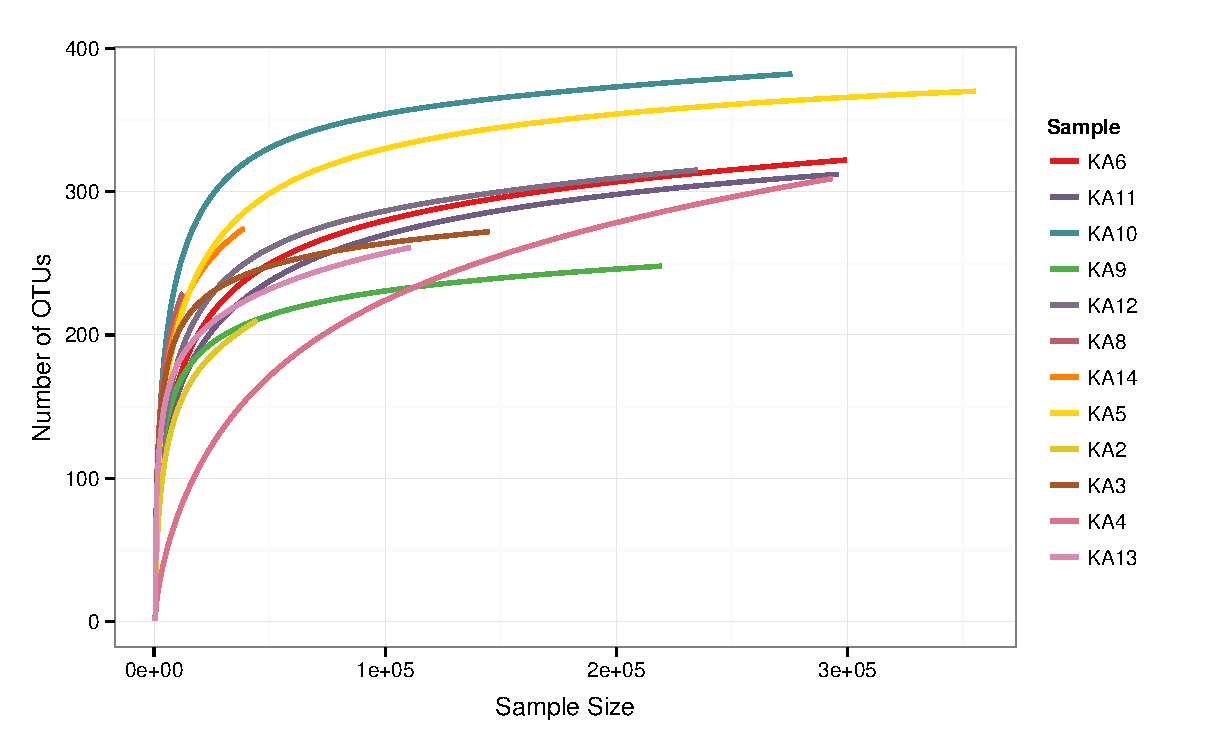
\includegraphics[width=1\textwidth]{./figures/Chapter_6/Figure_1_talkaled.eps}
  	\caption{Representativeness of sampled gut microbiota. The number of Operating Taxonomic Units (OTUs) as a function of
the number of sampled sequences is reported. The sequences were sampled with a step size of 100 sequences in order to
generate smooth curves. The asymptotic trends of curves indicate that a reasonable number of reads has been generated
in order to inspect the diversity of each sample. The different end values indicates variable numbers of clustered
sequences per sample.\label{fig:1talkal}}
\end{figure}
The analysis of community diversity for each samples (Table~\ref{tab:2kaltal}) showed  the lowest values for all three indices (Richness, Shannon and Evenness) for KA6 sample (\textit{O. montagui}), while the highest values were reached by the other \textit{O. montagui} sample (KA3), for Shannon and Evenness and by \textit{S. pelecaniformis} (KA10) for Richness. However, no statistically significant differences were found in relation to both talitrid species and locality of sampling (Table SM2).\\
\begin{table}
\centering
\scriptsize
\begin{tabular}{ c c c c c c }
\hline
Species & Locality & code & Richness & Shannon H & Evenness\\
\hline\hline
{\itshape O. montagui} & S. Giovanni di Sinis (Cabras) & KA3 & 322 & 3.995 & 0.692\\
{\itshape O. montagui} & Maimoni (Cabras) & KA8 & 229 & 0.497 & 0.091\\
{\itshape O. stephenseni} & Piscadeddus & KA14 & 274 & 0.931 & 0.166\\
{\itshape O. stephenseni} & S. Giovanni di Sinis (Cabras) & KA6 & 366 & 2.846 & 0.482\\
{\itshape S. pelecaniformis} & Centro 1{\textdegree} Sassu (Arborea) & KA11 & 294 & 3.473 & 0.611\\
{\itshape S. pelecaniformis} & Centro 1{\textdegree} Sassu (Arborea) & KA9 & 338 & 2.207 & 0.379\\
{\itshape S. pelecaniformis} & Sa Rocca Tunda & KA10 & 430 & 3.957 & 0.653\\
{\itshape T. saltator} & Giorgino & KA2 & 413 & 3.485 & 0.579\\
{\itshape T. saltator} & Giorgino & KA4 & 205 & 0.783 & 0.147\\
{\itshape T. saltator} & Giorgino & KA5 & 311 & 1.790 & 0.312\\
{\itshape T. ugolinii} & Is arenas & KA & 372 & 3.120 & 0.527\\
{\itshape T. ugolinii} & Is arenas & KA12 & 287 & 2.564 & 0.453\\
\hline
\end{tabular}
\caption{Diversity indices of microbiota. Diversity indices of gut microbiota in the twelve metabarcoding samples.\label{tab:2kaltal}}
\end{table}

\subsubsection{Species-specific signatures of gut microbiota}
Numerous evidences indicate that animals co-evolve with their gut microbiota \cite{ley2008worlds}. Consequently, species-specific patterns in the metabarcoding data of gut microbiota of the talitrids amphipds were inspected. Figure~\ref{fig:2talkal} reports the CCA  results, which indicate the presence of clearly separate clusters for the five species under analysis (\textit{O. montagui}, \textit{S. pelecaniformis}, \textit{T. saltator}, \textit{T. ugolinii}, \textit{O. stephensenii}), then supporting the hypothesis that amphipod digestive tracts host species-specific bacterial communities, which may be related to both the phylogeny and to potential dietary differences among the amphipod species, as exemplified in vertebrates \cite{ley2008worlds}.\\
\begin{figure}[!tb]
	\centering
	\includegraphics[width=0.7\textwidth]{./figures/Chapter_6/Figure_2_talkaled.eps}
  	\caption{Species-specific signatures of gut microbial community composition. Canonical Correlation Analysis (CCA) based
on OTU assignments to the bacterial taxonomy.\label{fig:2talkal}}
\end{figure}
As recently proposed for soil bacterial communities \cite{barberan2011using}, network analysis of significant taxon co-occurrence patterns could be useful to decipher the structure of complex microbial communities. Several works have shown recently that network analysis of co-occurrence may allow to define community patterns in several environments (for examples \cite{berry2014deciphering, boutin2014inter, williams2014demonstrating, geng2014co} see). Consequently, to further inspect the species-specific signatures of our amphipod gut microbiota a network analysis was conducted on Pearson's correlations among OTUs. This analysis, coupled with a k-means clustering, highlighted the presence of five taxonomically differentiated groups (clusters) of co-occurring OTUs (Figure~\ref{fig:3talkal}), in particular concerning \textit{Proteobacteria}, \textit{Actinobacteria} and \textit{Firmicutes}. Such clusters showed different representation in the five amphipod taxa (Figure SM1). In particular, cluster 4 was practically absent in \textit{S. pelecaniformis}, while the other clusters showed both a high variability among species, as well as among samples within the same species.\\
\begin{figure}[!tb]
	\centering
	\includegraphics[width=0.9\textwidth]{./figures/Chapter_6/Figure_3_talkaled.eps}
  	\caption{Network-based signatures of species-specific microbiota composition. Correlation network of OTU assignments. Each connection stands for a high degree of correlation between the two OTUs connected (Spearman's correlation r {\textgreater} 0.6 and p-value {\textless} 0.05). The size of each node in the network is proportional to its degree (number of connection of the node). The color of each node corresponds to a cluster obtained with the MCL algorithm with an ``inflation value'' equal to 1.4 (see section~\ref{par:kalmatmet}). Clusters have been defined after a k-means clustering.\label{fig:3talkal}}
\end{figure}

\subsubsection{Taxonomic differences in gut microbiota among talitrid species}
To evaluate which bacterial taxa mostly contribute to the interspecific differences of gut microbiota, OTUs were then assigned to bacterial phylogeny (Table SM3). Figure~\ref{fig:4talkal} shows the overall representation of taxonomic composition of gut microbiota, which highlight similar patterns, among all samples, with differences both within the same species, and among species. In particular, it could be worth of mentioning that \textit{Verrucomicrobia} were present in four out of five species (absent from all \textit{S. pelecaniformis} samples), as well as the group \textit{Deinococcus/Thermus} absent in both \textit{Orchestia} species. \textit{Verrucomicrobia} are particularly intriguing since this phylum, closely related to \textit{Planctomycetes} and \textit{Chlamydiae}, is considered to be particularly frequent in nonhost-assocaited environments, as soil and waters \cite{buckley2001environmental,freitas2012global}. \textit{Verrucomicrobia} have been suspected to contribute to energy generation from fermentable substrates in the human gut \cite{arumugam2011enterotypes} and \textit{Verrucomicrobia} have been found as particularly abundant after antibiotic treatment \cite{dubourg2013high}. We cannot consequently exclude that \textit{Verrucomicrobia} (present in all but \textit{S. pelecaniformis} samples) may have a role in some hypothetical differential nutrient assimilation in those talitrid species and in differential resilience toward environmental disturbance, which is frequent in sandy beaches \cite{defeo2009threats, ugolini2012sandhoppers, ugolini2005heavy, ugolini2008amphipod, ungherese2010relationship, moffett1998impact}.\\
\begin{figure}[!tb]
	\centering
	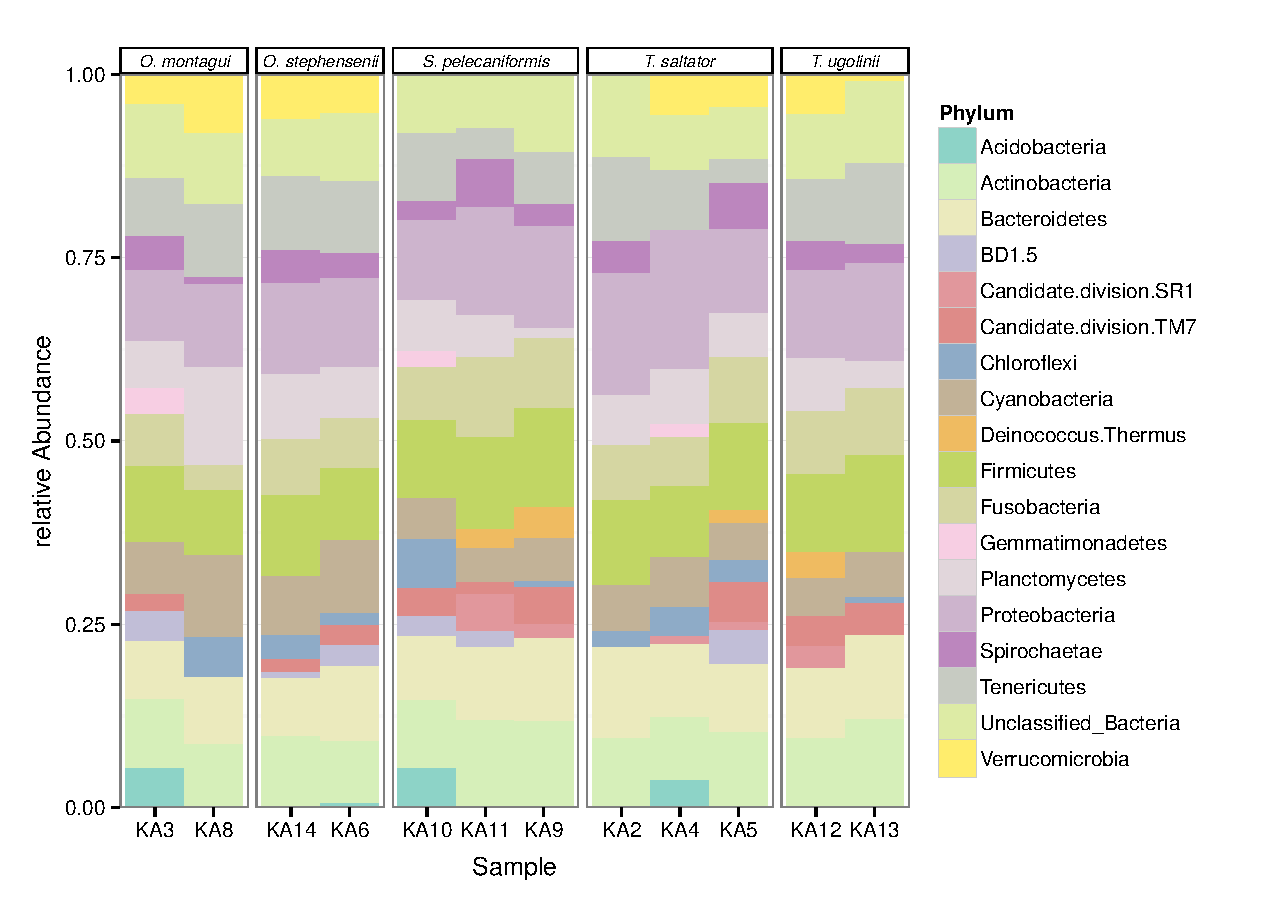
\includegraphics[width=1\textwidth]{./figures/Chapter_6/Figure_4_talkaled.eps}
  	\caption{Taxonomic composition of gut microbiota. Relative abundances barplot showing the relative abundance of bacterial phyla in each gut sample.\label{fig:4talkal}}
\end{figure}
To more in deep clarify the relative contribution of each phylum in species-specific gut microbiota signatures, a similarity percentage (simper) analysis was conducted (Table~\ref{tab:3kaltal}, Table SM3). In general, the phyla mostly contributing to differences between talitrid species are the most abundant, as \textit{Proteobacteria} (5.5\%-9.1\%), \textit{Firmicutes }(5.2\%-9.0\%), \textit{Bacteriodetes} (5.0\%-6.3\%), and \textit{Actinobacteria} (4.9\%-8.6\%). Interestingly, \textit{O. montagui}, which inhabits within the Posidonia banquettes  and macroalgae mat, shows the highest percentage of variance for \textit{Planctomycetes} in all pairwise comparisons, as well as among the highest percentage of variance for \textit{Firmicutes} also. \textit{Planctomycetes} have been found to densely populate the alkaline part of the hindgut of soil-feeding termites (\textit{Cubitermes} spp.) \cite{kohler2008novel} and to strongly vary with diet in humans \cite{cayrou2013molecular}. Moreover, \textit{Planctomycetes} constitute a large part of bacterial biofilms found on macroalgae \cite{lage2014planctomycetes}. The relative importance of \textit{Firmicutes} and \textit{Planctomycetes} in differentiating \textit{O. montagui }gut\textit{ }microbiota from those of the other talitrid species, may be due to the habitat of this species, possibly linked to the potential higher cellulose content of its diet. Of course confirmatory experiments under controlled conditions are needed to better evaluate the relative contribution of diet with respect to species in determining the specific of \textit{O. montagui }gut microbiota, especially in comparison with \textit{O. stephenseni}, which has been found in syntopy in the S. Giovanni di Sinis site (KA3 and KA6, Table~\ref{tab:1kaltal}).\\
\begin{landscape}
\begin{table}
\centering
\tiny
\begin{tabular}{ p{0.04\textwidth} p{0.04\textwidth} p{0.04\textwidth} p{0.04\textwidth} p{0.04\textwidth} p{0.04\textwidth} p{0.04\textwidth} p{0.04\textwidth} p{0.04\textwidth} p{0.04\textwidth} p{0.04\textwidth} p{0.04\textwidth} p{0.04\textwidth} p{0.04\textwidth} p{0.04\textwidth} p{0.04\textwidth} p{0.04\textwidth} p{0.04\textwidth} p{0.04\textwidth}}
\hline
 & Acido\-bacte\-ria & Actino\-bacte\-ria & Bacte\-roide\-tes & BD1.5 & SR1 & TM7 & Chlo\-rofl\-exi & Cyano\-bacte\-ria & Denico\-ccus/Ther\-mus & Fir\-micu\-tes & Fuso\-bacte\-ria & Placto\-myce\-tes & Proteo\-bacte\-ria & Spir\-ocha\-ete & Tene\-ricu\-tes & Unclas\-si\-fied & Verruco\-micro\-bia & Gemmati\-monade\-tes\\
\hline\hline
Os vs Sp & 0.65\% & 5.94\% & 5.54\% & 0.11\% & 0.11\% & 0.11\% & 0.66\% & 0.64\% & 0.11\% & 5.86\% & 0.36\% & 2.41\% & 7.81\% & 0.20\% & 0.34\% & 0.33\% & 0.53\% & NA\\
Os vs Tu & NA & 5.58\% & 4.99\% & 0.13\% & NA & 0.13\% & 0.13\% & 0.89\% & 0.12\% & 5.23\% & 0.54\% & 2.70\% & 6.82\% & 0.16\% & 0.40\% & 0.40\% & 0.69\% & NA\\
Os vs Om & 0.36\% & 6.50\% & 5.75\% & 0.17\% & NA & NA & NA & 1.16\% & NA & 8.68\% & 0.70\% & 6.10\% & 7.03\% & 0.21\% & 0.31\% & 0.51\% & 0.70\% & NA\\
Os vs Ts &NA & 7.73\% & 5.69\% & 0.15\% & NA & 0.15\% & 0.30\% & 0.59\% & NA & 7.02\% & 0.74\% & 2.80\% & 9.09\% & 0.26\% & 0.43\% & 0.42\% & 0.65\% & NA\\
Sp vs Tu & 0.67\% & 4.88\% & 5.07\% & 0.10\% & 0.10\% & NA & 0.70\% & 0.77\% & 0.09\% & 5.45\% & 0.32\% & 1.75\% & 6.20\% & 0.29\% & 0.17\% & 0.35\% & 0.23\% & NA\\
Sp vs Om & 0.57\% & 7.23\% & 6.34\% & 0.16\% & 0.16\% & 0.15\% & 0.31\% & 1.06\% & 0.15\% & 9.02\% & 1.00\% & 5.14\% & 6.94\% & 0.35\% & 0.35\% & 0.43\% & 0.34\% & 0.12\%\\
Sp vs Ts & 0.27\% & 8.24\% & 5.94\% & 0.15\% & 0.15\% & 0.14\% & 0.86\% & 0.56\% & 0.14\% & 8.23\% & 0.80\% & 1.25\% & 8.07\% & 0.45\% & 0.29\% & 0.44\% & 0.07\% & NA\\
Tu vs Om & 0.29\% & 7.88\% & 5.78\% & 0.17\% & NA & 0.17\% & NA & 1.14\% & NA & 8.89\% & 0.95\% & 5.66\% & 5.73\% & 0.10\% & 0.31\% & 0.51\% & 0.40\% & NA\\
Tu vs Ts & NA & 8.58\% & 5.88\% & NA & NA & 0.15\% & 0.15\% & 0.76\% & 0.15\% & 8.23\% & 0.84\% & 1.61\% & 7.21\% & 0.17\% & 0.34\% & 0.50\% & 0.25\% & NA\\
Om vs Ts & 0.65\% & 7.16\% & 5.98\% & 0.18\% & NA & 0.18\% & 0.52\% & 0.86\% & NA & 9.03\% & 0.87\% & 6.23\% & 7.63\% & 0.31\% & 0.41\% & 0.51\% & 0.59\% & 0.14\%\\
\hline
\end{tabular}
\caption{Species-specificity of bacterial phyla. Results of simper analysis. The percentage of variance attributed to each phylum in pairwise comparisons of talitrid species is reported. In bold pairwise comparison with \textit{O. montagui}. Om,, \textit{O. montagui}; Sp, \textit{S. pelecaniformis}; Ts, \textit{T. saltator}; Tu, \textit{T. ugolinii}; Os, \textit{O. stephenseni}.\label{tab:3kaltal}}
\end{table}
\end{landscape}

\subsubsection{Cellulolytic bacteria may contribute to \textit{O. montagui} gut microbiota difference}
From the analysis of taxonomic pairwise differences in gut microbiota (Table~\ref{tab:3kaltal}), it emerged that among the most important bacterial phyla, those of \textit{Firmicutes} and \textit{Planctomycetes} were particularly related to possible dietary/habitat differences between \textit{O. montagui} and the other talitrids. Both \textit{Firmicutes} and \textit{Planctomycetes} includes cellulose-degrading strains \cite{kulichevskaya2007schlesneria, schwarz2001cellulosome}. Additionally, a large proportion of \textit{Actinobacteria}(Figure~\ref{fig:4talkal}), which are well known to include many cellulolytic strains \cite{ljungdahl1985ecology}, has been found in all talitrid species. These evidence raised the question if the proportion of cellulosolytic bacteria with respect to the total bacterial load of the gut, may indeed be different between amphipod talitrids. However, from the molecular point of view, it is difficult to have a global overview of all genes encoding cellulases in a sample. Cellulase systems are in fact complex assemblages of multifunctional glycosyl hydrolases \cite{schwarz2001cellulosome}. Many families of glycosyl hydrolases have been found \cite{lynd2002microbial}, hampering the possibility to develop universal primers for PCR detection of all known cellulases. However, family 48 glycosyl hydrolases are well represented in many model cellulolytic clostridia and actinobacteria \cite{lynd2002microbial, beloqui2010diversity}.Primer pairs have been developed for 48 glycosyl hydrolases genes identification and quantification in environmental samples \cite{izquierdo2010diversity,pereyra2010detection}, in particular for clostridia and actinobacteria \cite{izquierdo2010diversity}. Since in our study a considerable fraction of recovered taxa fall within both \textit{Firmicutes} and \textit{Actinobacteria} (approx. 25\% of reads) we decided to investigate the presence of family 48 glycosyl hydrolases genes in amphipod gut microbiota. Results of the qPCR analysis are reported in Table 4. Interestingly, \textit{O. montagui} gut samples contained a higher ratio of GHF48 genes/16S rRNA genes (considered as estimators of the total number of bacterial cells) with respect to the other talitrid species, suggesting that indeed the different microbiota present in \textit{O. montagui} gut may be partly related to a higher prevalence of feeding on cellulose-rich substrates by this species.\\

\subsection{Conclusions}
Talitrid amphipods inhabiting supralittoral environment obtain most of their food from stranded materials, which include debris of various origin, as death animal organisms, macroalgae and plants (as land plants and \textit{P. oceanica} in the Mediterranean sea) \cite{adin2003preferential, colombini2011food}. In particular, due to the presence of low digestible components including lignocellulosic compounds in macroalgae and plants, we can hypothesize that a cellulosolytic bacterial flora in the digestive tract of talitrids could contribute in cellulose degradation. Indeed, previous authors \cite{nuti1971microrganisms, olabarria2009intraspecific} reported the presence of cellulose-degrading bacterial strain in the gut of talitrid amphipods, supporting the hypothesis of the involvement of gut microbiota in carbon source assimilation by such species. Here, we indicate that among the sampled species, which colonizes different microhabitats, \textit{O. montagui} (which is found within \textit{Posidonia} and macroalgae banquettes) harbors a different gut microbiota with respect to the other species. The \textit{O. montagui} gut microbiota includes more taxa known to be involved in cellulose degradation and an analysis of family 48 glycosyl hydrolases (one of the cellulase genes) indicated that indeed \textit{O. montagui} gut harbor a higher number of cellulose-degrading cells than the other talitrids. We conclude that the different ecological behavior of \textit{O. montagui} (a colonizer of \textit{Posidonia} banquettes) could be related also to a different taxonomic and functional composition of its gut microbiota. We cannot however, a priori exclude that a contribution of host encoded glycosyl hydrolases to food digestion could be present in \textit{O. montagui} and in the other talitrid amphipods, as demonstrated for the marine isopod \textit{Limnoria quadripunctata} \cite{king2010molecular}. Moreover, since \textit{O. montagui} shows a low population structure, probably due to its high capacity of dispersion \cite{matthaeis2000isolation}, it remains to explain the quite relevant differences between the two pools of specimens of \textit{O. montagui} gut microbiota investigated here, with respect to those of the other species, as \textit{O. stephenseni}. Consequently, further investigation will be needed to elucidate the differences between \textit{O. montagui} and \textit{O. stephenseni} gut microbiomes and  the relative influence of diet on gut microbial communities.\\

\subsection{Acknowledgments}
We are grateful to the directions of the Protected Marine Areas ``Penisola del Sinis e Mal di Ventre'' and ``Capo Carbonara'' for authorization to samplings and logistic support and to Marco Confalone for technical assistance during DNA extraction. We are also indebted with Dr. D. Bellan--Santini (Centre d'Oc\'{e}anologie de Marseille-DIMAR) for her help in the identification of some amphipod specimens. This work was supported by a grant from Regione Autonoma della Sardegna (L.R. 7/8/2007, N.7), code CRP-28345 and by a grant to KFAA from the Libyan Government. GB is supported by a PhD fellowships from CRA-RPS.\\

%%-----------
%% Backmatter
%%-----------
\backmatter
\chaptermark{Bibliography}
\renewcommand{\sectionmark}[1]{\markright{#1}}
\bibliographystyle{unsrt}                           %Use alpha codes for references
\sectionmark{Bibliography}
\addcontentsline{toc}{chapter}{Bibliography}        %Force addition of Bibliography to TOC    
\bibliography{References}

\mainmatter
\newthumb
%%%%%%%%%%%%%%%%%%%%%%%%%%%%%%%%%%%%%%%%%%%%%%
\logvartrue
\chapter{Microbiome in human disease}
%%%%%%%%%%%%%%%%%%%%%%%%%%%%%%%%%%%%%%%%%%%%%%
The interest in the role of the microbiome in human health has increased over the past decade, in conjunction with the development of new technologies for exploring complex microbial communities. The large-scale dynamics of the microbiome can be described by many of the tools and observations used in several studies of population ecology. Deciphering the human microbiome and its taxonomic signatures can also be used to deeply understand the properties of the microbial communities inside the human body and their correlation with human diseases. Therefore, both the microbiome and metagenome probably have important functions in health and disease and their exploration is a new challenge in human genetics.\\

\section{Changes in Cystic Fibrosis Airway Microbial Community Associated with a Severe Decline in Lung Function}
Cystic fibrosis (CF) is a genetic disease resulting in chronic polymicrobial infections of the airways and progressive decline in lung function. To gain insight into the underlying causes of severe lung diseases, we aimed at comparing the airway microbiota detected in sputum of CF patients with stable lung function (S) versus those with a substantial decline in lung function (SD). Microbiota composition was investigated by using culture-based and culture-independent methods, and by performing multivariate and statistical analyses. Culture-based methods identified some microbial species associated with a worse lung function, i.e. \textit{Pseudomonas aeruginosa}, \textit{Rothia mucilaginosa}, \textit{Streptococcus pneumoniae }and \textit{Candida albicans}, but only the presence of \textit{S. pneumoniae }and \textit{R. mucilaginosa }was found to be associated with increased severe decline in forced expiratory volume in 1 second (FEV\textsubscript{1}). Terminal-Restriction Fragment Length Polymorphism (T-RFLP) analysis revealed a higher bacterial diversity than that detected by culture-based methods. Molecular signatures with statistically significant odds ratio for SD status were detected, and classified as \textit{Pseudomonas}, \textit{Burkholderia} and \textit{Shewanella}, while for other Terminal Restriction Fragments (T-RFs) no species assignation has been achieved. The analysis of T-RFLP data by using ecological biodiversity indices showed reduced Evenness in SD patients compared to S ones, suggesting an impaired ecology of the bacterial community in SD patients. Statistically significant differences of ecological biodiversity indices among the three sub-groups of FEV\textsubscript{1 }(normal/mild \textit{vs} moderate \textit{vs} severe) were also found, suggesting that the patients with moderate lung disease have been experiencing changes in the airway assembly of taxa. Overall, changes in CF airway microbial community associated with a severe lung function decline were detected, allowing us to define some biomarkers (discriminatory species as well as some discriminatory T-RFs) as good candidates for the development of future predictors of substantial decline in lung function.\\

\subsection{Introduction}
Cystic fibrosis (CF) is the most frequent autosomal recessive life-threatening disease affecting 70'000 individuals worldwide, resulting in a progressive lung function decline. Currently, the percentage predicted forced expiratory volume in 1 s (FEV\textsubscript{1}\%) is commonly used to monitor lung function in CF and represents the best available predictor of survival for patients with CF \cite{taylor2012understanding}. While a decline in lung function is common in almost all CF patients, the rate of decline is highly variable \cite{rosenbluth2004lung}. Several studies have evidenced that some CF patients' FEV\textsubscript{1} seriously decline despite antibiotic treatment \cite{sanders2010failure} and that both long- and short-term fluctuations in lung function can be related to the disease severity due to CFTR gene mutations, chronic bacterial infection, and periodic pulmonary exacerbation \cite{rosenbluth2004lung}. It has been found that, although the age and the FEV textsubscript{1}\% can help predict the relative severity of an individual CF phenotype, they do not necessarily provide a good prediction of the \textit{risk} that a subject may run of a future rapid disease progression \cite{konstan2007risk}. Interpreting the significance of changes in FEV\textsubscript{1}\% over time requires a first more in-depth comprehension of the airway microbial community composition \cite{milla1998risk}.\\
Recent evidences have revealed that CF airway infections are polymicrobial \cite{stressmann2011analysis} and that the microbiota, as a collective entity, may contribute to pathophysiologic processes associated with chronic airway disease \cite{huang2011emerging}, \cite{rogers2014respiratory}. It has been suggested that the bacterial community composition may be a better predictor of disease progression than the presence of stand-alone opportunistic pathogens \cite{rogers2010determining}.\textcolor[rgb]{0.2,0.2,0.2}{ }Changes in airway bacterial community structures varied greatly upon exacerbations, decline in pulmonary health, antibiotic treatment, patient age increasing (for review, see \cite{lynch2013cystic, zhao2014modeling, mahenthiralingam2014emerging}). According to Carmody and colleagues \cite{carmody2013changes}, certain genera appear to play an important role in driving  change in airway bacterial community composition at reacutization and, therefore, might represent biomarkers for pulmonary exacerbation. Given the importance of lung function in  CF patients health, it is by extension important to understand the complexity of CF microbiota in those patients showing a severe decline in lung function and identify those factors associated with higher/lower pulmonary function decline. To date, it is largely unknown which factors contribute to the loss in FEV\textsubscript{1}, especially in clinically stable CF patients. The presence of organisms not typically considered CF pathogens, in addition to the ``typical'' CF pathogens \cite{hauser2011clinical}, may significantly affect the course and outcome of CF lung disease and may be responsible of the progressive decline in lung function \cite{sibley2009relevance}. Defining the microbial taxa associated with significant worsening of lung disease is only a first step in understanding their role in CF progression and provides novel insights into lung disease that could guide clinical management.\\ 
In this study we compared the airway microbiota detected in sputum from individual patients who have showed an important drop in FEV\textsubscript{1}\% in the previous year (a rate of FEV\textsubscript{1} decline greater than -5\% predicted per year) and did not respond to the conventional antimicrobial therapy (SD), versus that detected in sputum from stable (S) CF patients. All patients (S and SD) enrolled in the study were clinically stable, without any pulmonary exacerbation and antibiotic i.v. or oral therapy in the previous 4 weeks before specimen collection. Microbiota composition of a total of 78 patients attending three CF Centers in Italy was investigated by using culture-based methods, including anaerobic cultivation, Terminal Restriction Fragment Length Polymorphism (T-RFLP) analysis, and multivariate and statistical analysis. The primary objective was to achieve a better understanding of species/taxon bacterial diversity in SD and S patients and shifts in the dominant community members across the lung function decline. Since in routine microbiology laboratories, microbial detection and identification traditionally rely on culture-dependent methods for both bacteria and fungi, we further aimed at evaluating the role of  cultured yeast and filamentous fungi in a more rapid decline in pulmonary function and worse clinical outcomes.\\

\subsection{Materials and methods}

\subsubsection{Ethics Statement}
Sputum samples from patients with CF were collected at Bambino Ges\`u Children's Hospital (Rome, Italy), Cystic Fibrosis Center, Meyer Children's Hospital (Florence, Italy) and Giannina Gaslini Children's Hospital (Genoa University, Genoa, Italy), in accordance with the ethical guidelines. The study was approved by the local Ethics Committee of each participating Center [Prot. 85 of February 27, 2014 (Meyer Children's University Hospital); Prot. n. 681 CM of November 2, 2012 (Bambino Ges\`u Children's Hospital); Prot. n FCC 2012 Partner 4-IGG of September 18, 2012 (Giannina Gaslini Institute)]. Informed written consent was obtained from all subjects aged 18 years and over and from parents of all subjects under 18 years of age prior to enrollment in the study. The study protocol was in accordance with the Guidelines of the European Convention of Human Rights and Biomedicine for Research in Children and to those of the Ethics Committees of Bambino Ges\`u, Meyer and Giannina Gaslini Hospitals. All measures were taken to ensure patient data protection and confidentiality.\\

\subsubsection{Patients}
Seventy-eight patients were enrolled in the study between September 2012 and April 2013. These Institutions in Italy collectively provide care to a total of 680 patients (adult and children) with an average FEV textsubscript{1} decline of -1.44\% predicted/year. Patients, who had been diagnosed with CF according to the published Guidelines \cite{farrell2008guidelines}, were treated according to current standards of care with at least four microbiological controls per year \cite{flume2009cystic}. Patients were eligible if they could be classified as clinically stable, without any pulmonary exacerbation and antibiotic i.v. or oral therapy in the previous 4 weeks before specimen collection \cite{ramsey1999intermittent, fuchs1994effect}. Since pulmonary function testing cannot generally be successfully performed until children reach 6 years of age, only CF patients older than 6 years were enrolled. The annualized rate of FEV\textsubscript{1} decline was used to stratify patients. The rate of decline in pulmonary function was determined from each patient's best percentage of predicted FEV\textsubscript{1} (FEV\textsubscript{1}\%) over the last year. The difference between the best FEV\textsubscript{1}\% registered in the previous year and the best FEV\textsubscript{1}\% in the year before that was considered to group patients. CF patients were categorized as ``stable'' (S), i.e. with a rate decline in FEV\textsubscript{1} value not greater than -1,5\% per year, and with a ``substantial decline'' (SD) in FEV\textsubscript{1}, i.e. a rate of FEV\textsubscript{1} decline greater than -5\% predicted per year, and not responding to the conventional antimicrobial therapy (chronic suppressive antibiotic and/or i.v. antibiotics treatments). In order to assess the influence of FEV\textsubscript{1} status on the airway microbiota, S and SD patients were further categorized in three sub-groups: group I, CF patients with normal lung function or mild lung disease (FEV\textsubscript{1}\% {\textgreater} 70); group II, CF patients with a moderate lung disease (70 $\geq$ FEV\textsubscript{1}\% $\geq$ 40); group III, CF patients with a severe lung disease (FEV\textsubscript{1}\% {\textless} 40). FEV\textsubscript{1} values were measured according to the American Thoracic Society - European Respiratory Society standards \cite{miller2005standardisation}.\\

\subsubsection{Sample processing}
The analysis of the bacterial community composition was performed on spontaneously expectorated sputum (SES) samples since sputum specimen represents by far the most widely used sample in productive patients \cite{rogers2010determining}. Upon expectoration, CF sputum samples were immediately treated for 15 min with Sputolysin (Calbiochem, La Jolla, CA) in accordance with the manufacturer's instructions and split into aliquots for cultured and molecular analyses. Aliquots for culturable analysis of anaerobic bacteria were transferred within 15 min to an anaerobic cabinet for processing, according to Tunney et al. 2008 \cite{tunney2008detection}. Aliquots for culturable analysis of aerobic/microaerophilic bacteria and fungi were immediately examined, and the remaining aliquots were frozen and stored at -80{\textdegree}C for subsequent DNA extraction and molecular investigations.\\

\subsubsection{Bacteria and fungi detection by culture-methods}
\paragraph{Media and growth conditions} To detect aerobic and facultative anaerobic microbes, 10 {\textmu}l aliquots of serial 10-fold sputa dilutions up to 10\textsuperscript{{}-6} were prepared in 0.45\% (w/v) NaCl  and plated onto Columbia agar with 5\% sheep blood (CBA), MacConkey agar (MAC), Mannitol salt-agar (MSA), Chocolate agar with and without bacitracin (CHOC + BAC and CHOC), Columbia CNA agar with 5\% sheep blood (CNA), Pseudosel agar (PA),  \textit{Burkholderia cepacia} Selective Agar (BCSA), and Brain heart infusion (BHI) agar. Plates were incubated at 37{\textdegree}C for 48 h aerobically, with the exception of CHOC, CHOC+BAC and CNA cultures, which were incubated in presence of 5\% CO\textsubscript{2} \cite{burns1998microbiology}. BCSA cultures showing no growth after 48 h of incubation were re-incubated for a further 5 days.\\
Anaerobic cultures were carried out by plating 10 {\textmu}l aliquots of serial 10-fold sputa dilutions up to 10\textsuperscript{-6} prepared in quarter-strength Ringers lactate, supplemented with 0.05\% (w/v) L-cysteine, on the following anaerobic media: CDC anaerobic blood-agar (CABA), Kanamycin-Vancomycin Laked Blood-Agar (KVLBA), Phenylethyl alcohol agar (PEA), Veillonella neomycin agar, Cadmium Sulfate Fluoride Acridine Trypticase (CFAT) agar and \textit{Fusobacterium }selective agar (FSA). All plates were incubated anaerobically from 5 to 7 days at 37{\textdegree}C in an anaerobic work station (MACS MG-500, Don Whitley Scientific LTD) with an atmosphere of 85\% N\textsubscript{2}, 10\% H\textsubscript{2} and 5\% CO\textsubscript{2} at 37{\textdegree}C. Single colonies of each distinct morphotype were tested for oxygen sensitivity. Obligate anaerobes were defined as those isolates capable of growing anaerobically but not aerobically. Yeasts and filamentous fungi recovery was made by inoculating 10 {\textmu}l aliquots of digested sample on Sabouraud Dextrose agar (SAB) with and without chloramphenicol (SAB \-+\textsuperscript{ }CAF and SAB). Plates were incubated for 14 days at 30{\textdegree}C.\\
\paragraph{Microorganism identification} All the colony morphotypes observed on the selective and non-selective media were identified by appearance (colonial morphology, pigment production, $\beta $-haemolysis on sheep's blood agar, growth temperature), biochemical assays and/or proteomic profiling by matrix assisted laser desorption-time of flight mass spectrometry (MALDI-TOF MS) \cite{seng2013identification}. Both macroscopic and microscopic characters have been taken into account for the identification of yeasts and moulds. Ambiguous fungal strains were resolved by MALDI-TOF MS \cite{del2012maldi}. Aerobic and anaerobic bacterial isolates not resulting in species identification were characterized by means of molecular methods such as the amplification and sequencing of 16S rRNA and \textit{recA} genes and species-specific PCRs \cite{bittar2010detection}.\\

\subsubsection{DNA extraction}
About 400 {\textmu}l aliquots of frozen sputum were subjected to genomic DNA extraction using the Qiagen QIAamp DNA Mini Kit. Sample aliquots were spun at 10'000{\texttimes}g to pellet cellular material. After removal of the supernatant, cell pellets were re-suspended in 180 {\textmu}l of the appropriate enzyme solution [20 mg/ml lysozyme (Sigma) in 20 mM Tris-HCl (pH 8.0), 2 mM EDTA and 1.2\% Triton], incubated for 30 min at 37{\textdegree}C and then processed according to the manufacturer's protocol. Quantity and purity of extracted DNA were checked by NanoDrop (NanoDrop Technologies, USA) and gel electrophoresis.\\

\subsubsection{PCR amplification, and T-RFLP profiling}
The universal primers 926r (5'-CCG\-TCA\-ATT\-CAT\-TTG\-AGT\-TT-3') and 8f-6FAM (5'-AGA\-GTT\-TGA\-TCC\-TGG\-CTC\-AG-3') were used for amplification of the bacterial 16S rRNA gene \cite{stressmann2011analysis} following a previously reported protocol \cite{rogers2004characterization}. Every sputum DNA sample was subjected to three independent PCRs, and the resulting products were pooled and purified by GE Healthcare Sephadex G-100 for T-RFLP analysis. Two hundred nanograms of each purified PCR product were digested with 10 units of \textit{CfoI} at 37{\textdegree}C for at least 5 h. Approximately 20 ng of digested PCR product were injected into an ABI 3730 DNA Analyzer (Applied Biosystems), using LIZ1200 (Applied Biosystems) as size standard. Automated sequencing was performed by Genechron sequence service (Genechron Laboratory, Ylichron S.r.l., Rome, Italy).\\

\subsubsection{Statistical and bioinformatic analysis}
T-RFLP profiles were processed with PeakStudio \cite{mccafferty2012peak} to derive a matrix (Xt) with T-RFs sizes (binned at {\textpm}1 bp) and T-RFs intensities, as previously reported \cite{pastorelli2011effects, bacci2014composition}, which allow an estimation of beta diversity indices. Culture-based identification were transformed in a binary matrix (Xc) for presence (1) / absence (0) of each taxon. Both T-RFLP and culture-based matrices were then used for subsequent statistical analyses. For community diversity parameters, Richness, Evenness and Shannon indices were computed, as implemented in the software Past \cite{hammer2001past} on Xt and Xc matrices. Principal Component Analyses (PCAs) were computed on \textit{Xt} and \textit{Xc} matrices with the software R package by using as centroids both taxa or TFRs in relation to the analysis of culturable microflora and T-RFLP, respectively. For biplot analyses, new matrices derived from \textit{Xt} and \textit{Xc} were produced collapsing all samples from the same FEV\textsubscript{1} group or pulmonary status (S and SD); 95\% confidence ellipses were computed as scores for PCA. One-way ANOVA with Tukey \textit{post-hoc} comparison was performed with R package.\\ 
Conditional Maximum Likelihood Estimates (CMLE) of Odds ratio (ORs) and 95\% confidence Intervals (CI) were computed with OpenEpi suite (\href{http://www.openepi.com/}{http://\-www.\-openepi\-.com}). ORs were also estimated by applying a logistic regression model taking into account possible confounders, such as age, BMI, gender, CFTR genotype with R package. Putative taxonomic assignment of T-RFLP peaks was then performed on the T-RFLP profiles by using the web platform MiCA \cite{shyu2007mica} employing the T-RFLP Analysis (PAT+) option used to search for peak matching was performed on Ribosomal Database 10 (containing 1'519'357 bacterial 16S rRNA genes) with defaultparameters.\\

\subsection{Results}

\subsubsection{Patients and FEV{\textsubscript{1}} groups}
A total of 78 CF patients (39 males and 39 females, mean age 26.99 years) were enrolled (40 S and 38 SD), according to their lung function degree (Table~\ref{tab:epidtrflp}). Characteristics of S and SD cohorts, including CFTR genotype, gender, age, FEV\textsubscript{1}\%, body Mass Index (BMI), and nebulised antibiotics or oral azithromycin treatment are provided in Tables SM1 and SM2.\\
\begin{table}
\centering
\scriptsize
\begin{tabular}{l c c c}
\hline
Characteristics & All Patients & Stables  & Substantial-decliners \\
\hline\hline
Enrolled CF patients  & (n=78) & (n=40) & (n=38)\\
 &  &  & \\
Sex (n) & 39 male & 22 male & 17 male\\
        & 39 female & 18 female & 21 female\\
 &  &  & \\
\textit{CFTR} genotype, n (\%) &  &  & \\
F508del/F508del & 22 (28.20\%)  & 11 (27.5\%) & 11 (28.95\%)\\
F508del/other  & 34 (43.6\%) & 18 (45\%) & 16 (42.10\%)\\
Other/other & 22 (28.20\%) & 11 (27.5\%) & 11 (28.95\%)\\
 &  &  & \\
Mean age + SD  & 26.99 {\textpm} 11.56  & 27.57 {\textpm}11.71  & 26.33 {\textpm}11.51\\
 &  &  & \\
Mean value of FEV\textsubscript{1}\% + SD  & 59.70 {\textpm} 25.02  & 64.35 {\textpm} 28.39  & 54.81 {\textpm} 20.13\\
 &  &  & \\
Disease stage categories, n (\%) &  &  & \\
Normal/mild (FEV\textsubscript{1}\% {\textgreater} 70) & 30 (38.46\%) & 17 (42.5\%) & 13 (34.21\%)\\
Moderate (70 ${\geq}$ FEV\textsubscript{1}\% ${\geq}$ 40) & 27 (34.62\%) & 14 (35\%) & 13 (34.21\%)\\
Severe (FEV\textsubscript{1}\% {\textless} 40) & 21 (26.92\%)  & 9 (22.5\%) & 12 (31.58\%)\\
\hline
\end{tabular}
\caption{Demographic and clinical characteristics of all participants and in stable (S) and substantial-decliners (SD) status.\label{tab:epidtrflp}}
\end{table}

\subsubsection{Culture microbiota in S and SD patients}
Seventy-eight specimens, obtained in accordance with the ethical Guidelines during the course of routine medical care, were processed by culture-dependent approaches, including the classical microbiological approach in accordance with the Guidelines for CF sputum analysis and advanced approaches for the identification of bacterial isolates, anaerobic bacteria, and fungi. The occurrence of all microbial taxa, not only those known to be involved in pulmonary infections, was used to determine if a single taxon or an assemblage of them may be associated with SD or S status.\\
\begin{figure}[!tb]
	\centering
	\includegraphics[width=0.8\textwidth]{./figures/Chapter_7/Figure_1_cond_taxa}
  	\caption{\label{fig:fig1condtaxa}Biplot of the principal component analysis of culturable taxa from 78 specimens of stable (S) and substantial decliners (SD) patients with CF. Ellipse with 95\% CI is reported. Numbers on axes indicate the amount of variance explained by each component. Labels outside the 95\% ellipse have been jittered to avoid overlaps.}
\end{figure}
Principal Component analysis (PCA) of the culturable microflora detected from S and SD samples did not reveal any clear distinction between S and SD groups, neither among the three different clinical conditions examined (I, normal/mild lung disease; II, moderate disease; III, severe disease) (Figure S1). Interestingly, when PCA was performed using the detected taxa as centroids, differences in the microbial community composition between S and SD groups were found. Figure~\ref{fig:fig1condtaxa} shows that \textit{Pseudomonas aeruginosa}, \textit{Rothia mucilaginosa}, \textit{Streptococcus pneumoniae, }and \textit{Candida albicans} for SD group, the absence of fungi and \textit{Staphlyoccoccus aureus} for S group are the most important taxa in contributing to variance differences among S and SD patients in our dataset (in terms of taxa outside the confidence ellipse 95\%, which group  the most similarly occurring taxa).\\
\begin{table}
\centering
\scriptsize
\begin{tabular}{l c c}
\hline
a) SD vs. S patients &  & \\		
Taxon & OR & CI 95\% (lower - upper) \\
\hline\hline
Streptococcus pneumonia & \textbf{9.95} & \textbf{1.47 - 233.90} \\
Rothia mucilaginosa & \textbf{4.87} & \textbf{1.03 - 38.80} \\
Pseudomonas aeruginosa & 1.66 & 0.66 - 4.20 \\
Candida albicans & 1.04 & 0.39 - 2.79 \\
Staphylococcus aureus & 0.86 & 0.34 - 2.18 \\
absence of fungi & 0.77 & 0.30 - 1.96 \\
  &  &  \\
b) FEV\textsubscript{1} (III) vs. FEV\textsubscript{1} (I) + (II) &  & \\
Taxon & OR & CI 95\% (lower - upper) \\
\hline\hline
Candida albicans & 1.57 & 0.53 - 4.55 \\
Pseudomonas aeruginosa & 1.46 & 0.40 - 4.94 \\
No anaerobic bacteria & 1.46 & 0.40 - 4.94 \\
\hline
\end{tabular}
\caption{\label{tab:ortrflp}Odds Ratio from culturable microflora with differential occurrence in SD and S patients and FEV\textsubscript{1} groups. Data report the taxa detected from Principal Component Analysis (Figure~\ref{fig:fig1condtaxa}), the Odds Ratio (OR) of association between presence of the taxa and SD status (a) or FEV\textsubscript{1} (III) with respect to a cohort composed by FEV\textsubscript{1} (I) and FEV\textsubscript{1} (II) patients (b), the 95\% confidence intervals (CI 95\%). Statistically significant ORs are reported in bold. FEV\textsubscript{1}, group I = normal/mild (FEV\textsubscript{1}\% {\textgreater} 70); FEV\textsubscript{1}, group II = moderate (70 ${ \geq}$ FEV\textsubscript{1}\% ${\geq}$ 40); FEV\textsubscript{1}, group III = severe (FEV\textsubscript{1}\% {\textless} 40).}
\end{table}
To statistically evaluate the relationships between the differential presence of these taxa and the patients' status, Odds Ratio (ORs) were computed (Table~\ref{tab:ortrflp}). Statistically significant ORs for SD were found for the presence of \textit{S. pneumoniae} (OR=9.954) and \textit{R. mucilaginosa} (OR=4.867) (Table~\ref{tab:ortrflp} (a)). However, taking account the possible confounders in a logistic regression (Table SM3) for \textit{S. pneumonia }OR was 1.12 (CI 0.14-6.11) and \textit{R. mucilaginosa} OR was 7.37 (CI 1.45-44.41). In the same model \textit{P. aeruginosa} OR was 1.14 (CI 0.34-3.87), while \textit{C. albicans, S. aureus }and absence of fungi had ORs of 2.30, 1.04 and 0.57, respectively.\\
\begin{figure}[!tb]
	\centering
	\includegraphics[width=0.8\textwidth]{./figures/Chapter_7/Figure_2_fev1_taxa}
  	\caption{\label{fig:fig2fev1taxa}Biplot of the principal component analysis of culturable taxa from 78 specimens of patients with CF considering their FEV\textsubscript{1} groups. Ellipse with 95\% is reported. Numbers on axes indicate the amount of variance explained by each component. Labels outside the 95\% ellipse have been jittered to avoid overlaps.}
\end{figure}
When the three different FEV{\textsubscript{1}} groups were considered, PCA showed a differential occurrence of \textit{Achromobacter xylosoxidans},\textit{P. aeruginosa},\textit{C. albicans} as well as the absence of an anaerobic microflora in CF patients with severe lung disease (group III) (Figure~\ref{fig:fig2fev1taxa}). Conversely, for the presence of \textit{A. xylosoxidans} no statistical support could be obtained, since this species was detected only in one patient of group III. Considering ORs for the FEV\textsubscript{1} of group III, in comparison with FEV \textsubscript{1} I and II groups (Table~\ref{tab:ortrflp} (b)), no statistically significant ORs were detected between culturable microflora and FEV\textsubscript{1} decline. By applying a logistic regression including confounders the same result was found (Table SM4), with no detectable limit for the lower confidence interval.\\
\begin{table}
\centering
\scriptsize
\begin{tabular}{l c c c}
\hline
Bacterial communities & \multicolumn{3}{c}{Diversity indices} \\
\hline\hline
a) Culturable microflora & Shannon & Evenness & Richness \\
\hline
SD & 1.64 {\textpm} 0.39 & 0.37 {\textpm} 0.06 & 5.6 {\textpm} 2.3 \\
S & 1.65 {\textpm} 0.40 & 0.36 {\textpm} 0.06 & 5.7 {\textpm} 2.4 \\
  &  &  &  \\
b) T-RFLP community profiles &  &  \\
\hline
SD & 1.89 {\textpm} 0.55 & 0.43 {\textpm} 0.18\textsuperscript{a} & 19.8 {\textpm} 11.0 \\
S & 1.86 {\textpm} 0.56 & 0.52 {\textpm} 0.18\textsuperscript{b} & 16.5 {\textpm} 10.8 \\
  &  &  &  \\
c) T-RFLP profiles / FEV\textsubscript{1} groups &  &  \\
\hline
FEV\textsubscript{1} group I & 1.95 {\textpm} 0.49\textsuperscript{a} & 0.45 {\textpm} 0.17 & 19.7 {\textpm} 9.5 \\
FEV\textsubscript{1} group II & 1.59 {\textpm} 0.48\textsuperscript{b} & 0.47 {\textpm} 0.22 & 15.1 {\textpm} 11.9 \\
FEV\textsubscript{1} group III & 2.09 {\textpm} 0.61\textsuperscript{a} & 0.53 {\textpm} 0.15 & 19.6 {\textpm} 11.6 \\
\hline
\end{tabular}
\caption{Diversity estimates for bacterial communities in sputum samples of CF patients. Data show the mean indices for substantial decliners (SD) and stable (S) patients {\textpm} standard deviation. For T-RFLP data, the indices for the three FEV\textsubscript{1} groups are also reported. Different letters indicate statistically significant (P{\textless}0.05) differences after one-way ANOVA and Tukey \textit{post-hoc} comparison.\label{tab:divtrflp}} 
\end{table}
Concerning the overall values of diversity indices, no statistically significant differences in alpha diversity values were found between the whole groups of SD and S patients (Table~\ref{tab:divtrflp} (a)) as well as between SD and S patients belonging to the severe group (FEV\textsubscript{1} group III), and among the three FEV{\textsubscript{1}} sub- roups in both SD and S patients (data not shown). Furthermore, no significant correlation was found between diversity indices and FEV\textsubscript{1} values (as Pearson's r, p value was \textless 0.9 for all indices).\\

\subsubsection{Total microbiota in S and SD CF patients}
\paragraph{Community composition: species absence/presence} In the 78 sputum samples analyzed by T-RFLP, a total of 1411 bands representing 208 different T-RF lengths were detected. The number of individual bands in each sample ranged from 2 to 43. In particular, ranges were from 3 to 43 for the S patients and 2 to 39 for the SD patients. The mean number of T-RF bands per patient in S sample set (20.2 {\textpm} 11.4) was higher than that of the SD sample (15.5 {\textpm} 10.2), though the difference was not significant (P {\textless} 0.06). Among the 208 T-RF bands detected, 82 (39.4\%) were ``singletons'' defined here as bands that occurred in only one sample. Singletons were detected in 18 (45\%) S and 10 (27.2\%) SD samples.\\
\paragraph{Bacterial community structure} PCA carried out on single patient's T-RFLP profiles did not reveal any clear differences between S and SD patients, nor any differences associated with lung disease status (Figure SM1). When PCA was performed on the markers (T-RFs) as centroids, several (16) T-RFs with a differential contribution toward SD and S (as those outside the confidence ellipse at 95\%) were found (Figure~\ref{fig:fig3condtrf}). Identified T-RFs outside the 95\% confidence ellipse in the biplot were putatively assigned to bacterial taxa by \textit{in silico} digestion with \textit{Cfo}I, using the Phylogenetic Assignment Tool (PAT+) provided by Microbial Community Analysis III (MiCA 3) (\href{http://mica.ibest.uidaho.edu/}{http://mica\-.ibest\-.uidaho\-.edu}). Phylogenetic assignment of the T-RFs was grouped at the phylum level.\\ 
\begin{figure}[!tb]
	\centering
	\includegraphics[width=0.8\textwidth]{./figures/Chapter_7/Figure_3_cond_trf}
  	\caption{\label{fig:fig3condtrf}Principal Component Analysis of total occurrences of T-RFs in 78 patients with CF from S and SD patients. Ellipse with 95\% is reported. Comparison of stable with substantial-decliners CF patients. Numbers on axes indicate the amount of variance explained by each component. Labels outside the 95\% ellipse have been jittered to avoid overlaps.}
\end{figure}
One T-RF (920-922 nt) resulted to have a higher impact on the variance of SD status, while another T-RF (482-484 nt) contributed more to the variance of S status. Moreover, the T-RF at 692-694 nt was only detected in SD patients (in eight out of 38 patients, corresponding to approx. 21\%). A query launched on MiCA 3 web server against the database of 16S rRNA gene sequences allowed to putatively assign 10 out the above mentioned 16 T-RFs to known bacterial taxa. To statistically evaluate the relationships between the differential presence of these taxa and the patients' status, ORs were computed for TFs, too (Table~\ref{tab:ordettrflp}). In particular, T-RFs with OR {\textgreater} 1 (Table~\ref{tab:ordettrflp} (a), i.e., more present in SD than in S patients) enabled to detect \textit{Pseudomonas}, \textit{Shewanella}, and \textit{Burkholderia}. Interestingly, a T-RF putatively assigned at \textit{Shewanella - Colwellia} (920-922 nt) resulted with a high OR for SD patients. The logistic regression model was well in agreement with CMLE ORs estimates (Table SM5). However, several T-RFs were not assigned to any known cultured taxon nor can be assigned to any 16S rRNA gene sequence present in the database (unidentified), including the T-RF at 482-484 nt which is indicated as more frequent in S patients (OR {\textless} 1).\\
\begin{table}
\centering
\tiny
\begin{tabular}{l c c l}
\hline
TRF size (nt) & OR & CI 95\% (lower - upper) & Putative taxonomic attribution \\
\hline\hline
a) SD vs S &  &  &  \\	
\hline
30-32 & 0.94 & 0.26 - 3.39 & Burkholderia \\
32-34 & 2.05 & 0.79 - 5.51 & Burkholderia, Streptomyces \\
34-36 & 0.79 & 0.31 - 1.98 & Anaerofilum, uncultured \\
94-96 & 0.56 & 0.21 - 1.43 & Chloroflexi, Bacteroidetes, uncultured \\
96-98 & 0.28 & 0.06 - 1.06 & Pseudoalteromonas, uncultured \\
98-100 & 0.93 & 0.33 - 2.64 & Cycloclasticus, Mannheimia, uncultured \\
150-152 & 2.04 & 0.83 - 5.15 & uncultured \\
206-208 & 1.18 & 0.44 - 3.17 & Pseudomonas, uncultured \\
482-484 & \textbf{0.29} & \textbf{0.08 - 0.88} & unidentified \\
572-574 & 1.25 & 0.50 - 3.13 & Pseudomonas, Shewanella \\
574-576 & 1.04 & 0.40 - 2.68 & Shewanella \\
584-586 & 0.72 & 0.29 - 1.79 & uncultured \\
586-588 & 2.04 & 0.83 - 5.15 & unidentified \\
588-590 & 0.89 & 0.36 - 2.20 & unidentified \\
692-694 & n.d. & n.d. - n.d. & unidentified \\
920-922 & 3.61 & 1.06 - 14.37 & Shewanella, Colwellia \\
 &  &  & \\
b) FEV\textsubscript{1} (III) vs FEV\textsubscript{1} (I)+(II) &  &  \\
\hline
208-210 & 2.36 & 0.84 - 6.74 & Pseudomonas \\
194-196 & 2.55 & 0.96 - 6.87 & uncultured \\
234-236 & 2.09 & 0.80 - 5.52 & unidentified \\
572-574 & 2.11 & 0.81 - 5.77 & Pseudomonas, Shewanella \\
96-98 & \textbf{3.00} & \textbf{1.00 - 10.18} & Pseudoalteromonas, uncultured \\
574-576 & 2.15 & 0.78 - 6.34 & Shewanella \\
586-588 & 1.50 & 0.59 - 3.86 & unidentified \\
360-362 & 1.47 & 0.57 - 3.77 & uncultured \\
98-100 & 2.10 & 0.68 - 7.23 & Cycloclasticus, Mannheimia, uncultured \\
206-208 & 1.66 & 0.59 - 4.94 & Pseudomonas, uncultured \\
32-34 & 1.01 & 0.38 - 2.73 & Burkholderia, Streptomyces \\
30-32 & 1.22 & 0.33 - 5.06 & Burkholderia \\
34-36 & 0.70 & 0.26 - 1.83 & Anaerofilum, uncultured \\
560-562 & 0.36 & 0.11 - 1.09 & Cellvibrio, Pseudomonas, uncultured \\
470-472 & 0.40 & 0.10 - 1.33 & uncultured \\
558-560 & \textbf{0.28} & \textbf{0.07 - 0.90} & Halomonas \\
144-146 & \textbf{0.07} & \textbf{0.00 - 0.42} & uncultured \\
150-152 & \textbf{0.25} & \textbf{0.09 - 0.66} & uncultured \\
\hline
\end{tabular}
\caption{\label{tab:ordettrflp} Odds ratio from TRFs with differential occurrence in S and SD patients and FEV\textsubscript{1} groups. Data report the TRFs size in nucleotides (nt), the CMLE Odds Ratio (OR) estimates of association between presence of the TRF and SD status (a) or FEV\textsubscript{1} (III), the 95\% confidence intervals (CI 95\%) and the putative taxonomic attributions with MiCA web server. The reported attributions indicate the main hits retrieved for that particular size. Statistically significant ORs are reported in bold.} 
\end{table}
PCA biplot (Figure~\ref{fig:fig4fev1trf}) showed that the vector of FEV\textsubscript{1} group I has a different orientation with respect to those of the other FEV textsubscript{1} groups, suggesting that some T-RFs can indeed be differentially present. We then computed ORs for the 18 T-RFs outside the ellipse 95\%. Results are reported in Table~\ref{tab:ordettrflp} (b). One T-RF (96-98 nt) resulted to contribute more to the variance of FEV\textsubscript{1} group III, while three T-RFs (558-560 nt, 144-146 nt, 150-152 nt) contributed more to the variance of FEV\textsubscript{1} I and II groups. Putative taxonomic identification carried out on such T-RFs highlighted that most of them cannot be assigned (as uncultured or unidentified). The T-RF at 558-560 nt can indeed be assigned to \textit{Halomonas}. However, though CMLE ORs (Table~\ref{tab:ordettrflp} (b)) showed significant ORs the logistic regression model (Table SM6) did not show supported the data.\\
\begin{figure}[!tb]
	\centering
	\includegraphics[width=0.8\textwidth]{./figures/Chapter_7/Figure_4_fev1_trf}
  	\caption{\label{fig:fig4fev1trf} Principal Component Analysis of total occurrences of T-RFs in 78 patients with CF from S and SD patients. Ellipse with 95\% is reported. Comparison among FEV\textsubscript{1} groups (I, II, III). Numbers on axes indicate the amount of variance explained by each component. Labels outside the 95\% ellipse have been jittered to avoid overlaps.}
\end{figure}

\paragraph{Diversity indices} To investigate changes in bacterial communities that may have occurred with severe decline in lung function, diversity indices were computed for all samples by using community ecology parameters (beta diversity estimates). Results revealed that the Evenness, i.e. the equal distribution of T-RFs, resulted higher in S sample set (0.52 {\textpm} 0.18) than in SD sample set (0.43 {\textpm} 0.18) (p {\textless} 0.05). The other diversity indices considered (Richness and Shannon) were not statistically different between the whole dataset of S and SD patients (p {\textgreater} 0.05) (Table~\ref{tab:divtrflp} (b)), and no statistically significant changes were observed between S and SD groups when considering the three FEV\textsubscript{1} sub-groups separately (data not shown). The diversity indices (Evenness, Richness) values did not allow to detect differences among the three FEV textsubscript{1} groups (Table~\ref{tab:divtrflp} (c)), while significant (p{\textless}0.05) differences in Shannon indices of FEV\textsubscript{1} (II) \textit{vs} FEV\textsubscript{1} (I) and of FEV\textsubscript{1} (II)\textit{vs} FEV textsubscript{1} (III) were found. However, no significant differences were found for FEV\textsubscript{1} (I) \textit{vs} FEV\textsubscript{1} (III).\\

\subsection{Discussion}
In the present study, we used both culture-dependent methods for detection of aerobic and anaerobic bacteria and fungi, and a culture-independent method by terminal restriction fragment length polymorphism (T-RFLP), which provide a fingerprint of the most highly abundant members of the community. Data presented here provide new insights into the CF airway microbiota of S and SD patients, population dynamics of the microbiota following lung disease status (normal/mild, moderate and severe lung disease), ecology of the bacterial communities related to lung function decline and establishment of specialized communities of pathogens associated with poor pulmonary function, including putative discriminant microbial species and T-RFs for S and SD groups.\\
The percentage predicted forced expiratory volume in 1 s (FEV\textsubscript{1}\%) is currently the gold standard measure of disease severity in patients with CF. The rate at which FEV\textsubscript{1} declines over a period is an indicator of aggressiveness of a patient's lung disease, regardless of the stage of the patient's lung disease (normal/mild, moderate and severe) \cite{zhao2012decade}. In the present work, we defined as a substantial decline in lung function a decrease of 5\% or more in FEV\textsubscript{1} predicted per year. This percentage drop in FEV\textsubscript{1} suggests a substantial decline similar to that defined by Vandenbranden and colleagues \cite{vandenbranden2012lung} and twice the one reported in published studies \cite{sanders2010failure}. Therefore, the microbiota investigation in CF patients with a more substantial decline in lung function over the previous year can be very useful in order to try to understand where a pathogen is only a marker of disease severity or an independent contributor to the loss of lung function \cite{milla1998risk}.  As ultimately the goal of pulmonary interventions is to retard the disease process and therefore reduce the rate of lung function decline, defining new potential biomarkers for the early detection of severe rate of decline in lung function could be essential for making rational decisions regarding intervention.\\
The presence of \textit{P. aeruginosa} in respiratory tract cultures has been previously reported to be associated with a more rapid decline in lung function, especially when mucoid phenotype is present \cite{emerson2002pseudomonas}. However, Vandenbranden and colleagues \cite{vandenbranden2012lung} found that the presence or absence of \textit{P. aeruginosa} or mucoid \textit{P. aeruginosa} was not predictive of lung function decline. Our findings from culture-based analysis showed that \textit{P. aeruginosa} cannot be strongly proposed as indicative of severe decline in lung function (OR = 1.14, CI 0.34-3.87). It is noteworthy that maintenance treatment for chronic \textit{P. aeruginosa} with inhaled antibiotics and/or azithromicin in accordance with the Guidelines \cite{34}. resulted in slowing down the rate of decline in FEV\textsubscript{1}. Our culture-based results suggest an important role of \textit{S. pneumoniae} and \textit{R.mucilaginosa} as marker species for SD status. Although \textit{S.pneumoniae} is a common respiratory tract pathogen, it is unusual in CF \cite{foweraker2009recent}. This bacterial species is able to persist in the CF lung and has been recently regarded as pathogenic within the CF community \cite{maeda2011population}. However, to the best of our knowledge, it is still unclear whether \textit{S.pneumoniae} has a role in acute exacerbation and severe lung decline or can act synergically with other CF pathogens. As regards \textit{R. mucilaginosa}, it was previously reported as an aerobic species isolated from CF sputum \cite{tunney2008detection} and it was defined by several Authors \cite{bittar2008molecular} \cite{39} as a ``new'' emerging CF pathogen. Recently, Lim and colleagues \cite{lim2013mechanistic} confirmed that \textit{R. mucilaginosa} is present and metabolically active in the lungs of CF patients and that it evolves and adapts to each patient's lung environment over the course of a persistent infection. Our results also reinforce the previous findings of Chotirmall and colleagues \cite{chotirmall2010sputum} who reported that colonization with \textit{C. albicans} presages FEV\textsubscript{1} decline in CF. Although the same Authors suggested the implication of \textit{C. albicans} in the decline of CF lung function, the clinical relevance of yeasts is still a matter of debate, and has yet to be confirmed. Our findings add support to $i)$ the pathogenicity of species derived from the oral cavity and usually considered as clinically insignificant, and $ii)$ the complex interaction between typical pathogens and microbiota, such as the association between \textit{P. aeruginosa} and anaerobes/fungi.\\
It is well known that CF airways harbor numerous organisms that evade detection by culture-based methods. To carefully examine the microbiota from patients with stable versus worsening disease status, we chose to utilize T-RFLP analysis to generate community profiles. T-RFLP is a popular molecular profiling technique with the capacity to resolve community members based on the position of restriction sites in the 16S rRNA gene \cite{liu1997characterization}. T-RFLP profiles have been extensively used for community differentiation, identification of specific organisms in microbial populations  and comparison of the relative phylotype richness and community structure in a diverse range of environments \cite{osborn2000evaluation, marsh2005culture, tiquia2010using, joo2010monitoring, nakano2010prediction}. When previously applied to the analysis of spontaneously expectorated sputum from CF patients, T-RFLP has indicated the presence of a diverse array of bacterial species \cite{stressmann2011analysis, rogers2010determining, rogers2003bacterial, sibley2008polymicrobial}. In this study, we used T-RFLP analysis as a tool to investigate two key topics. First, do the bacterial communities (microbiota) detected in S samples differ from those in SD samples? Additionally, are there differences in the microbiota among CF patients with different status of lung disease? Results obtained in the present study by T-RFLP analysis revealed a greater bacterial diversity within sputum samples than that detected by culture approaches. We did not find T-RFLP profiles exclusive of the patients from S or SD groups. T-RFLP analysis revealed sixteen T-RFs as the most differentiating between S and SD groups after PCA. However, in our dataset, significant ORs were only recorded for two of them (and only one was possible to identifiy as putative \textit{Shewanella})Interestingly, the other T-RFs which differentiate (tough not significantly on the basis of ORs) S from SD were putatively identified as belonging to known CF pathogens, as \textit{Pseudomonas} and \textit{Burkholderia}, but most of them resulted in no species assignation (only {\textasciitilde}18\% of T-RF band lengths match a band length generated from published sequence data).Therefore, these unknown T-RFs could be either novel species or related species/strains of the core community of CF airways, but with enough heterogeneity in the 16S rRNA gene that may generate slightly different fragment sizes \cite{camarinha2012validating}. \textit{S.pneumonia} and \textit{R. mucilaginosa} were detected by culturing but not by T-RFLP analysis. It is well known that molecular methods based on 16S sequence data have a limited ability to resolve taxonomic identification at the species level \cite{filkins2012prevalence} and may introduce biases during the primer-binding step of PCR \cite{cai2013biased}. In spite of these limits, and taking also into consideration that T-RFLP only allows a putative (though fast) taxonomic assignment, this culture-independent method adds valuable information to the data obtained from culture analysis. To gain a more comprehensive characterization of CF lung microbial communities, more sophisticated and expensive techniques, such as bacterial metabarcoding by 16S rDNA and metagenomic sequencing \cite{maughan2012analysis, lim2014clinical} will be applied. \\
To investigate changes in bacterial communities that may have occurred with substantial decline in lung function, the diversity indices on T-RFLP data were calculated for all samples. Diversity provides a measure of community complexity based on the number (Richness) and relative abundances (Evenness) of the species present. The reduced Evenness observed in SD respect to S group of patients revealed an impaired ecology of the bacterial community in SD patients, which in turn can be associated with lung function decline experienced by those patients. When we assessed community structures to describe the degree of change occurring in the airway microbiota following the decline in lung function, we did not find a decrease in Shannon diversity index with advanced disease in the SD group. As suggested by Zhao and colleagues \cite{zhao2012decade}, other factors, such as antibiotic use, rather than lung function or patient age have been found to be the primary drivers of the decreasing bacterial diversity in CF patients with progressive lung disease. In our study, patients with a more rapid decline in lung function did not have a higher antibiotic exposure over the previous year with respect to S patients; additionally, both S and SD patients did not receive antibiotics in the 30 days preceding the specimen collection. Collectively, our results suggest that the antibiotic use is not likely to have contributed to the failure in detecting a decrease in community diversity with advanced disease in the SD group. Moreover, we cannot \textit{a priori} exclude that the use of relative peak intensities as a proxy for taxa frequency, though largely used (for instances see  \cite{camarinha2012validating, blackwood2007interpreting, ding2013community}), may be someway biased and can produce altered data. Our analyses suggest that overall bacterial diversity remains relatively stable despite the decreasing in relative abundances of the species in SD patients. Indeed, as previously stated by Zhao and colleagues \cite{zhao2012decade}, community diversity alone is not a sufficient indicator of the disease status. However, considering only the three subgroups of FEV\textsubscript{1} (normal/mild \textit{vs} moderate, \textit{vs} severe), independently from the rate at which FEV textsubscript{1}\% declines, statistically significant differences among the three sub-groups were also found, suggesting that the patients with intermediate FEV\textsubscript{1} values are experiencing changes in the airway assembly of taxa. A more detailed taxonomic and functional analysis of the microbial community of lung microbiota of CF patients could help elucidating the microbial factors that can contribute to such changes.\\ 
In conclusion, by combining culture-dependent and culture-independent methods with ecological tools and clinically relevant information, a more comprehensive view of microbial community composition in SD patients with CF was determined. Overall, our results suggest that the presence of \textit{P. aeruginosa} ``per se'', as well as the single T-RFLP profiles, are not able to define the S or SD group. New biomarkers are required in CF to predict the decline clinical phenotype and monitor the response of CF patients to existing and new therapeutic strategies. Microbial factors represent a potential to provide biomarkers for the early detection of the substantial lung function decline in CF. We have identified some discriminatory species as well as some discriminatory T-RFs, that represent good candidates as predictors of substantial decline in lung function, enabling to stratify individuals with CF at high or low risk of future severe lung function decline. However, only longitudinal studies can help determine patterns of association between the CF airway microbiome and lung disease. A more in-depth investigation of microbial airway bacterial communities in longitudinal studies and by high-throughput sequencing and bioinformatics tools will provide powerful means to better understand the contribution of the airway microbiome to severe decline in FEV\textsubscript{1} and its potential for the development of new biomarkers as predictors of severe pulmonary disease in CF patients.\\

\subsection{Acknowledgements} We thank John LiPuma, Gianni Mastella and late Gerd D\"oring for their helpful suggestions. We dedicate the present article to the memory of Gerd D\"oring (University of T\"ubingen, T\"ubingen, Germany), who was a world authority on infection and inflammation in the CF lung. With Gerd's death, we lost an excellent scientist, a loyal and generous friend, a marvelous speaker, and a charming person of great sensitivity and nobility. We also acknowledge the Italian Cystic Fibrosis Research Foundation (FCC) for its support and administrative tasks, and Graziana Manno, Anna Marchese, Silvia Campana, Gabriella Ricciotti, Cristina Cantale for their valuable assistance. \\

%%%%%%%%%%%%%%%%%%%%%%%%%%%%%%%%%%%%%%%%%%%%%%%%%%%%%%%%%%%%%%%%%%%%%%%%%%%%%%%%%%%%%%%%%%%%%%%%%%%%%%%%%%%%%%%%%%%%%%%%%%%%%%%%%%%%%%%%
%%%%%%%%%%%%%%%%%%%%%%%%%%%%%%%%%%%%%%%%%%%%%%%%%%%%%%%%%%%%%%%%%%%%%%%%%%%%%%%%%%%%%%%%%%%%%%%%%%%%%%%%%%%%%%%%%%%%%%%%%%%%%%%%%%%%%%%%

\section{Taxonomic signatures of CF airway microbiota distinguish between stable and severe declining patients}
Cystic fibrosis (CF) is an autosomal recessive genetic disorder characterized by a progressive decline in lung function. Patients with CF may show a rapid and severe decline of their pulmonary efficiency, measured as FEV\textsubscript{1} percentage, despite antibiotic treatment. Usually, these treatments are selected relying on the susceptibility of individual and culturable microbial strains to specific antibiotics in vitro. Nevertheless, this approach may not correctly predict medical outcomes because of both technical and biological factors. In these years, several culture-independent studies have shown that the CF airway infection is significantly more complex and dynamic than previously detected. Thus, understanding the ecological and evolutionary dynamics able to modify the lung microbiota of CF patients is critically important for either developing new and more effective therapies or improving existing ones. In this study, we analyzed the sputum from 52 patients with different disease conditions through 16S rRNA metabarcoding analysis in order to bring an in-depth overview of the lung microbiota at different stages of CF disease. The enrolled patients were divided into 2 main groups based on their rate decline in FEV\textsubscript{1} value per year. Patients with a rate decline greater than -1.5\% were assigned to the ``stable'' group (S), whereas patients with a rate decline between -1.5\% and -5.0\% were assigned to the ``severe decliners'' group (SD). Moreover, patients were further categorized into three FEV\textsubscript{1} groups: group I (FEV\textsubscript{1} {\textgreater} 70\%); group II (FEV\textsubscript{1} ranging from 40\% to 69\%) and group III (FEV\textsubscript{1} {\textless} 40\%). Surprisingly, the metabarcoding analysis has shown that bacterial biodiversity of stable patients dropped down passing from group I to group II of FEV\textsubscript{1} index; whereas bacteria community connection has a similar behavior passing from ``stable'' to ``severe decliners conditions''. Here, we theorize that something (still unknown) is occurring in the ecology of lung microbiota passing from FEV\textsubscript{1} I to FEV\textsubscript{1} II, which may misbalance bacterial community ecology, opening the way to more severe conditions.\\

\subsection{Introduction}
The main goal of pulmonary interventions is to retard the disease process reducing the rate of lung function decline even defining new potential biomarkers for the early detection of severe rate of decline in lung function, essential for taking rational decisions regarding intervention.\\
In recent years the microbial ecology of the airways in cystic fibrosis (CF) has been shown to be significantly more complex than originally considered \cite{lipuma2010changing, rogers2014respiratory}. Recent works using culture-independent identification methods have revealed that CF patients harbor a vast array of bacteria, previously not identified and not suspected to be involved in the infection and inflammation typical of CF patients \cite{zhao2012decade}. During the last few years, the development of next-generation sequencing technologies and bioinformatics tools has enabled the large-scale investigation of microbial communities and has facilitated our understanding of a ``black box'' of microbial communities present in CF airways \cite{delmont2011metagenomic}. These findings have altered drastically our understanding of CF lung disease \cite{rogers2014respiratory}, but their translation into improvements in clinical outcome remains a substantial obstacle to improving the quality of care. It has been proposed that the lung microbial communities might be considered as a unique distinct pathogenic entity, whose impact on the host may be greater than the combined impacts of its individual component species alone \cite{rogers2010comparing}. Indeed, an ecological perspective on multispecies colonization of the CF airways will permit to understand the role of polymicrobial dynamics in CF lung disease and provide the clinicians with new biomarkers of CF progression, as well as with new bacterial targets for antibiotic treatment \cite{sibley2008polymicrobial}.\\
Until now, many efforts have been made to identify microbes associated with airway diseases, antibiotic treatment, patient age increasing, and periodic pulmonary exacerbation \cite{zhao2012decade, cox2010airway, carmody2013changes, zhao2014modeling, zemanick2013inflammation}. However, it is still not clear how changes in the airway microbiota composition are predictive of severe lung disease progression. Bacterial infections in the CF airways are currently monitored through routine microbiology and CF patients receive cures based on culturable microbial pathogens colonizing their airways \cite{flume2009cystic}. It has been found that the administration of antimicrobial therapy, based on the in vitro susceptibilities of classic CF pathogens, does not necessarily correlate with the clinical outcome \cite{sibley2009relevance}.\\
Here we used 16S rRNA metabarcoding analysis of lung microbiota to describe the ecological issues (biological diversity, taxa composition, interaction among taxa) related to a specific pulmonary physiopathological status. We analyzed the microbiota of a large cohort of patients (a total of 52 patients) differing for status (S and SD) and FEV\textsubscript{1} index values in order to explore how bacterial communities change during the course of CF disease.\\

\subsection{Materials and Methods}

\subsubsection{Ethics Statement}
Sputum samples from patients with CF were collected at Bambino Ges\`u Children's Hospital (Rome, Italy), Cystic Fibrosis Center, Meyer Children's Hospital (Florence, Italy) and Giannina Gaslini Children's Hospital (Genoa University, Genoa, Italy), in accordance with the ethical guidelines. The study was approved by the local Ethics Committee of each participating Center [Prot. 85 of February 27, 2014 (Meyer Children's University Hospital); Prot. n. 681 CM of November 2, 2012 (Bambino Ges\`u Children's Hospital); Prot. n FCC 2012 Partner 4-IGG of September 18, 2012 (Giannina Gaslini Institute)]. Informed written consent was obtained from all subjects aged 18 years and over and from parents of all subjects under 18 years of age prior to enrollment in the study. The study protocol was in accordance with the Guidelines of the European Convention of Human Rights and Biomedicine for Research in Children and to those of the Ethics Committees of Bambino Ges\`u, Meyer and Giannina Gaslini Hospitals. All measures were taken to ensure patient data protection and confidentiality.\\

\subsubsection{Patients}
52 patients attending three Italian CF Centers (Bambino Ges\`u Children's Hospital, Rome; CF Center, Meyer Children's Hospital, Florence; and Giannina Gaslini Children's Hospital, Genoa) were enrolled in the study between September 2012 and April 2013. Patients, who had been diagnosed with CF according to the published Guidelines \cite{farrell2008guidelines}, were treated by following such Guidelines and consensus for lung monitoring with at least four microbiological controls per year \cite{flume2009cystic}. Patients were eligible if they could be classified as clinically stable, without any pulmonary exacerbation and antibiotic e.v. or oral therapy in the previous 4 weeks \cite{fuchs1994effect, ramsey1999intermittent}.\\
The annualized rate of FEV\textsubscript{1} decline was used to stratify patients as previously reported. CF patients were categorized as ``stable'' (S), i.e. with a rate decline in FEV\textsubscript{1} value no greater than -1.5\% per year, and with a ``substantial decline'' (SD) in FEV\textsubscript{1}, i.e. a rate of FEV\textsubscript{1} decline greater than - 5\% predicted per year. Both S and SD patients were further categorized in three FEV\textsubscript{1} groups: group I, CF patients with normal lung function or mild lung disease (FEV\textsubscript{1} {\textgreater} 70\%); group II, CF patients with a moderate lung disease (FEV\textsubscript{1} ranging from 40\% to 69\%); group III, CF patients with a severe lung disease (FEV\textsubscript{1} {\textless} 0\%). FEV\textsubscript{1} values were measured according to the American Thoracic Society-European Respiratory Society standards \cite{miller2005standardisation}. The overall description of the patient dataset is reported in Table SM1. For additional details on patients number and the number of sequences generated for each group of patients see Table~\ref{tab:ffc116s}.\\
\begin{table}
\centering
\scriptsize
\begin{tabular}{c c c c}
\hline
FEV1 & Condition & \# Patients & \# Sequences \\
\hline\hline
I & S & 13 & 35746 \\
II & S & 10 & 29462 \\
III & S & 6 & 19499 \\
I & SD & 10 & 31332 \\
II & SD & 7 & 20121 \\
III & SD & 6 & 21947 \\
Total &  & 52 & 158107\\
\hline
\end{tabular}
\caption{\label{tab:ffc116s}Number of enrolled patients in each group. The table reports also the number of amplicon sequences assigned to each group.} 
\end{table}

\subsubsection{Sample processing and DNA extraction} 
The analysis of the bacterial community composition was performed on spontaneously expectorated sputum (SES) samples since sputum specimen represents by far the most widely used sample in productive patients \cite{rogers2010comparing}. Samples processing was performed as previously described. About 400 {\textmu}l aliquots of frozen sputum were subjected to genomic DNA extraction using the commercially-available Kit QIAamp DNA Mini Kit. Sample aliquots were spun at 10,000{\texttimes}g to pellet cellular material. After removal of the supernatant, cell pellets were resuspended in 180 {\textmu}l of enzyme solution (20 mg/ml lysozyme in 20 mM Tris{\textperiodcentered}Cl, pH 8.0, 2 mM EDTA, 1.2\  Triton), incubated for 30 min at 37{\textdegree}C and then processed according to the manufacturer's protocol. Quantity and purity of extracted DNA were checked by NanoDrop (NanoDrop Technologies, USA) and PicoGreen fluorescent assay (Life Technologies) and gel electrophoresis.\\

\subsubsection{Amplification and barcoding of bacterial 16S rRNA gene amplicons}
Fifty-four samples (from 52 patients) were obtained and subjected to 16S rRNA gene amplification. The V3, V4, and 5 hypervariable regions of the 16S rRNA gene were amplified using primer 357F (5'-CTA\-CGG\-GAG\-GCA\-GCA\-G-3') modified with the addition of the 454 FLX-titanium adaptor ``B'' sequence (5'-CTA\-TCC\-CCT\-GTG\-TGC\-CTT\-GGC\-AGT\-CTC\-AG-3') and primer 926R (5'-CCG\-TCA\-ATT\-CMT\-TTR\-AGT-3') modified with the addition of 18 unique seven-nucleotide barcode sequences (MID 1 - MID 18, Roche MID adapters) and the 454 FLX titanium adaptor ``A'' sequence (5'-CCA\-TCT\-CAT\-CCC\-TGC\-GTC\-CAT\-CTC\-ATC\-CCT\-GCG\-TGT\-CTC\-CGA\-CTC\-AG-3').\\
Primer design and barcode sequences were as previously reported by Human Microbiome Project (HMP) Consortium \href{http://www.hmpdacc.org/tools\_protocols/tools\_protocols.php}{http://\-www\-.hmp\-dacc\-.org/\-tools\_proto\-cols/\-tools\_pro\-to\-cols\-.php}.\\
PCR amplification was performed on 30 {\textmu}g of DNA template in a total volume of 25 {\textmu}L containing 1{\texttimes} AccuPrime Buffer II (Life Technologies), 10 {\textmu}M of 357F fusion-primer, 10 {\textmu}M of 926F fusion-primer and 0.03 U/{\textmu}L AccuPrime High-Fidelity \textit{Taq} DNA polymerase (Life Technologies). PCR reactions were heated at 95 {\textdegree}C for 2 min followed by 30 cycles of 95 {\textdegree}C for 20 s, 55 {\textdegree}C for 30 s, and 72 {\textdegree}C for 5 min. All reactions were prepared in a sterile PCR hood. Three independent 25 {\textmu}L PCR reactions were generated for each patient DNA-template. Negative control reaction (no DNA template) were also performed. 2.5 {\textmu}L of each replicate reactions were examined by electrophoresis on an 1,5 \% agarose gel. PCR amplicons were cleaned using the Agencourt AMPure XP Beads according to the manufacturer's specifications (Beckman Coulter). To ensure removal of primers and any nonspecific amplicons, purified amplicon libraries were analyzed using the Agilent Bioanalyzer 2100 employing the Agilent DNA 1000 Kit. The concentration of the purified amplicons was determined using the Quant-iT PicoGreen dsDNA fluorescent assay Kit (Life Technologies).\\
For each patient sample, the three independent purified and quantified PCR reactions were pooled in an equimolar ratio of 109 molecules {\textmu}l-1. Amplicon pools were quantified using KAPA Library Quantification Kits (KAPA Biosystems) to determine exactly the number of amplifiable molecules in the amplicon libraries. For 16S Amplicon qPCR reactions two dilutions (1:500 and 1:1000) of each purified library were used. qPCR amplification was performed on 4 {\textmu}L of Amplicon library template in a total volume of 10 {\textmu}L containing 6 {\textmu}L of KAPA SYBR{\textregistered} FAST qPCR Master Mix. Reactions were heated at 95 {\textdegree}C for 5 min followed by 35 cycles of 95 {\textdegree}C for 30 s, and 60 {\textdegree}C for 90 s. In addition, dissociation (melt curve) analysis was performed to provide indication of possible primer- and/or adaptor-dimer contamination of libraries.\\ The concentration of each Amplicon library in molecule/{\textmu}L was achieved by inference from a standard curve generated using the six DNA Standard included in KAPA Library Quantification Kits.\\

\subsubsection{Amplicon Library Amplification and Pyrosequencing} 
To clonally amplify the amplicon libraries, the optimal amount of DNA to use in emPCR amplification was determined using emulsion titration procedure according to the supplier's instructions described in ``emPCR Amplification Manual'' (454 Life Sciences Roche Corporation). Before emulsion titration, MID-containing libraries (MID1 to MID18) were normalized to the same molecule concentration, pooled in equal volumes, and diluted to the emulsion PCR working concentration according to the supplier's instructions described in ``emPCR Amplification Manual'' (454 Life Sciences Roche Corporation). Overall, 3 equimolar amplicon library pools were prepared and purified with AMPure XP beads. Emulsion PCR, emulsion breaking and amplicon pyrosequencing were performed applying the 454 GS FLX+ chemistry following supplier protocols (454 Life Sciences Roche Corporation). Sequencing of amplicons was conducted on a 454 GS FLX+ System (454 Life Sciences Roche Corporation); each of the 3 amplified amplicon libraries was loaded on a PicoTiterPlate (PTP) device, using 3 regions of a medium regions ``4-lane'' gasket. The latest GS FLX+ software 2.9 version was used to sequencing and the pipeline 3 for long amplicon was used to data processing (454 Life Sciences Roche Corporation).\\

\subsubsection{Sequence processing and data generation}
Sequences generated via pyrosequencing were separated from the run according to their barcode sequence using custom bash and Java scripts available upon request. Sequences possessing primer mismatches higher than 2 bp were discarded in order to assign to each sample (patient) only sequences with an almost perfect match with the barcode. A quality check step was performed using StremingTrim 1.0 \cite{bacci2014streamingtrim} a very conservative algorithm able to retain as much information as possible. Sequences were then trimmed to a fixed length (568 - 572 bp) while low quality sequences were removed from the analysis. Processed sequences were subjected to the UPARSE pipeline \cite{edgar2013uparse} in order to remove chimeric sequences (both in de novo and in reference mode) and to cluster them into Operational Taxonomic Units (OTUs). An identity threshold of 97\% has been used in this step to be able to analyze the lung bacterial community at a high resolution level. Indeed, a 97\% identity threshold of the 16S rRNA gene corresponds approximately to the taxonomic level of species \cite{konstantinidis2007prokaryotic}. Representative sequences obtained from the UPARSE clustering were taxonomically classified using the SINA standalone classifier combined with the most recent SILVA database available (SSU 115). For additional details on the number of OTUs assigned to each patient see Table SM1.\\
OTU counts were normalized to relative abundance by dividing the number of assigned sequences by the sample size (number of sequences assigned to each patient) before comparing bacterial community from different samples. Prevalence values were calculated as the fraction of samples containing a given OTU whereas abundance values were computed as the fraction of reads assigned to a particular OTU. For taxonomic data generation, all OTUs assigned to the same taxa were summed together and normalized as described above.\\

\subsubsection{Statistical analyses}
OTUs counts were rarefied according to the lowest abundant sample in order to be able to compute and compare biodiversity indices of all samples. Shannon, Richness and Evenness indices were calculated on rarefied sequence counts repeating the rarefaction step 1000 times. An Analysis of Variance (ANOVA) has been performed to inspect differences in bacterial community diversity related to clinical conditions. In particular, Forced Expiratory Volume (FEV\textsubscript{1}) and patient conditions (Stable or Severe Decline) have been considered in the analysis. Moreover, to confirm results obtained with the ANOVA analysis, a Multivariate Analysis of Variance (MANOVA) was performed on the whole bacterial dataset. Finally, a Canonical Correlation Analysis (CCA) has been carried on to be able to visualize results and inspect the effect of the two factors reported above. Before performing the CCA analysis, the abundance (represented by number of sequences) of the OTUs was log transformed for normalization. All statistical analyses were performed with the R software \cite{team2012r} and the vegan package \cite{oksanen2007vegan}.\\

\subsubsection{Network construction}
In order to generate network representations of the lung bacterial community, all possible Spearman's rank correlation have been calculated between OTUs. A co-occurrence event has been considered valid only if the Spearman's correlation coefficient was higher than 0.6 and statistically significant with a p-value lower than 0.05. Two distinct networks were generated (one including Stable patients and the other considering Severe Decline patients) were each node correspond to a different OTU and each edge represent the presence of a statistically significant Spearman's correlation {\textgreater} 0.6 between OTUs. The diameter of the nodes was directly proportional to the OTU relative abundance in the dataset. The same approach has been used to construct other three networks, one for each FEV\textsubscript{1} level. All statistical analyses were carried out in the R environment using the igraph package for network generation.\\

\subsection{Results}
\subsubsection{Taxonomic description}
In the sputum microbiota analyzed a total of 44 OTU were detected, with values ranging from 1 to 4334 (Table SM2). The relative abundance values of each identified genus are reported in Figure~\ref{fig:fig116s}. A large heterogeneity was found for all patients, and such heterogeneity in relative taxa abundance was also present at higher taxonomic levels (Figure SM 1).\\
\begin{figure}[!tb]
	\centering
	\includegraphics[width=1\textwidth]{./figures/Chapter_7/Figure_1_16s}
  	\caption{\label{fig:fig116s}Segmented bar plot reporting relative abundances of OTU counts collapsed at Genus taxonomy level. OTU counts were transformed to relative abundance by dividing the number of assigned sequences by the sample size. Each bar of this plot reports the relative abundance of all genera detected in a sample (patient). The bar colors represent the different genera detected.}
\end{figure}
When the bacterial distribution at genus level was analyzed in terms of prevalence and abundance between groups (Figure~\ref{fig:fig216s}), similar patterns in all groups (S vs. SD at different FEV\textsubscript{1} groupings) were found for genera belonging to \textit{Actinobacteria}, \textit{Bacteroidetes}, \textit{Firmicutes} and \textit{Fusobacteria}. On the contrary, genera belonging to \textit{Proteobacteria }showed a more variable pattern. In particular, \textit{Pseudomonas} assignments within the SD group showed a pattern of increasing prevalence and abundance following FEV\textsubscript{1} groups. In the S group, \textit{Pseudomonas} assignments showed high levels of prevalence and abundance in the group II of FEV\textsubscript{1} only.\\ 
\begin{figure}[!tb]
	\centering
	\includegraphics[width=0.7\textwidth]{./figures/Chapter_7/Figure_2_16s}
  	\caption{\label{fig:fig216s} Abundance and prevalence of detected taxa in CF patients. Prevalence (intensity of color) and abundance (size) of clades in the lung microbiome. Taxa belonging to the same Phylum were grouped together reporting a different color for each Phylum detected.}
\end{figure}

\subsubsection{Statistical evaluation of lung microbiota differences}
Rarefaction curves (Figure~\ref{fig:fig316s}) showed that all samples had the required amount of sequences to assess OTU richness (all curves reached an asymptote). After normalization of bacterial counts to relative abundance values, biodiversity indices have been calculated (Table SM3) and a two-factor Analysis of Variance (two-factor ANOVA) was carried out in order to evaluate if biodiversity values differed in relation to both patient status (S vs. SD) and pulmonary functionality (FEV\textsubscript{1} groups) (Table~\ref{tab:ffc216s}). 
\begin{figure}[!tb]
	\centering
	\includegraphics[width=0.8\textwidth]{./figures/Chapter_7/Figure_3_16s}
  	\caption{\label{fig:fig316s} Rarefaction curves calculated for sputum samples of all patients. A curve has been drawn for each sample with the sample ID reported at the end. As showed in this figure, all curves reached an asymptote whereas samples have not achieved the same number of sequences.}
\end{figure}
Regarding both Evenness and Shannon indices, the two-factor analysis of variance showed no significant effect for the single factors, but their interaction was significant. On the contrary, Richness index showed a significant effect of the FEV\textsubscript{1} index, but no significant effect between S and SD groups (Table~\ref{tab:ffc316s}). Furthermore, a Tukey's HSD test has been performed for each index showing significant differences between group I and group II of FEV\textsubscript{1}. In particular, for Richness index a significant difference has been found passing from group I to group II of FEV\textsubscript{1} level, whereas, both for Shannon and Evenness indices, a significant difference has been found but only considering values from the S group (Figure SM2 and Table SM4).\\
\begin{table}
\centering
\scriptsize
\begin{tabular}{ c c c c c c c c } 
\hline
FEV & Condition & \multicolumn{2}{c}{Richness} & \multicolumn{2}{c}{Shannon} & \multicolumn{2}{c}{Evenness}\\
\hline\hline
  &  & Mean & St. Dev. & Mean & St. Dev. & Mean & St. Dev. \\
I & S & 23.5512 & 6.1071 & 2.2006 & 0.4976 & 0.7010 & 0.1202 \\
I & SD & 23.4139 & 3.7107 & 1.8466 & 0.4816 & 0.5859 & 0.1447 \\
II & S & 16.3694 & 6.5919 & 1.3104 & 0.6641 & 0.4693 & 0.2103 \\
II & SD & 18.1791 & 8.2644 & 1.7579 & 0.5979 & 0.6162 & 0.1252 \\
III & S & 23.7927 & 5.1791 & 2.2185 & 0.3820 & 0.7014 & 0.0783 \\
III & SD & 16.2788 & 8.2847 & 1.4349 & 0.7957 & 0.5015 & 0.2590 \\
\hline
\end{tabular}
\caption{\label{tab:ffc216s}Biodiversity indices means and standard deviations for each group of patients.} 
\end{table}
Subsequently, a two-factor multivariate analysis of variance (MANOVA) was conducted considering OTUs as dependent variables. Likewise the ANOVA analysis described above, we have used the same factors FEV\textsubscript{1} and condition (S and SD) to test the hypothesis that there would be differences in OTU counts between these groups. The condition factor showed a statistically significant effect, Pillais' Trace = 0.99, F approx = 8.82, p {\textless} 0.05 (for additional information see Table SM5).\\
\begin{table}
\centering
\scriptsize
\begin{tabular}{ r c c c c c l}
  &  &  &  &  &  &  \\
a) \hfill \textbf{Richness} & Df & Sum Sq & Mean Sq & F value & Pr(>F) & \\
\hline\hline
FEV1 & 2 & 416.5000 & 208.2300 & 4.8360 & 0.0124 & * \\
Condition & 1 & 10.9000 & 10.8800 & 0.2530 & 0.6175 & \\
FEV1:Condition & 2 & 117.5000 & 58.7500 & 1.3650 & 0.2656 & \\
Residuals & 46 & 1980.6000 & 43.0600 &  &  & \\
\hline
  &  &  &  &  &  & \\
b) \hfill \textbf{Shannon} & Df & Sum Sq & Mean Sq & F value & Pr(>F) & \\
\hline\hline
FEV1 & 2 & 2.9820 & 1.4909 & 4.4560 & 0.0170 &  * \\
Condition & 1 & 0.4250 & 0.4250 & 1.2700 & 0.2656 & \\
FEV1:Condition & 2 & 2.6800 & 1.3399 & 4.0050 & 0.0249 & * \\
Residuals & 46 & 15.392 & 0.3346 &  &  & \\
\hline
  &  &  &  &  &  & \\
c) \hfill \textbf{Evenness} & Df & Sum Sq & Mean Sq & F value & Pr(>F) & \\
\hline\hline
FEV1 & 2 & 0.1431 & 0.0715 & 2.6980 & 0.0780 & \\
Condition & 1 & 0.0326 & 0.0326 & 1.2310 & 0.2731 & \\
FEV1:Condition & 2 & 0.2515 & 0.1257 & 4.7420 & 0.0134 & * \\
Residuals & 46 & 1.2197 & 0.0265 &  &  & \\
\hline
\end{tabular}
\caption{\label{tab:ffc316s}Two-factor Analysis of Variance (ANOVA) of biodiversity indices. As reported in the table for both Shannon (b) and Evenness (c) indices, the analysis has shown a statistically significant effect of the interaction between the two factors considered (FEV\textsubscript{1} index and patient condition). On the other hand, regarding Richness index (a), the analysis has shown a significant effect of the FEV\textsubscript{1} index only. Any P value less than 0.05 has been marked with an asterisk to signal a statistically significant variation between groups.} 
\end{table}
In order to further investigate the dependence of bacterial community composition from patient conditions we perform a constrained Canonical-Correlation Analysis (CCA) using log normalized OTU counts (Figure~\ref{fig:fig416s}). CCA analysis results showed that both FEV\textsubscript{1} and condition factors, included in the analysis, were able to explain 15 \% only of the total variance, suggesting that this two factors were not able to discriminate the major taxa detected. However, CCA1 and CCA2 together explained more than 73 \% of the constrained inertia, denoting these two coordinates as acceptable candidates to represent the CCA results. As shown in Figure 4, there is a high level of overlap between samples (the gray ellipse), but, despite the low level of variance explained by the constrained CCA analysis, samples from group III of FEV\textsubscript{1} index constitute two distinct clusters. One cluster included patients from the S group and the other one contained patients from the SD group.\\
\begin{figure}[!tb]
	\centering
	\includegraphics[width=0.7\textwidth]{./figures/Chapter_7/Figure_4_16s}
  	\caption{\label{fig:fig416s}Results of Canonical Correlation Analysis. The dot colors represent the level of the FEV1 index, whereas the dot shapes correspond to patient condition (S or SD). The grey area shows the section of the plot with the highest level of overlap; on the other hand, two clusters with low level of overlap were reported using a dotted line. These clusters contain all samples from the FEV\textsubscript{1} III group divided according to their condition (S or SD).}
\end{figure}

\subsubsection{Network analysis}
In order to evaluate the presence of different co-occurrence patterns of OTUs in patients with different status (S and SD), a network of correlations between OTUs was built. This approach has been widely used to successfully explore the interaction between organisms from different environments and to study the association between organisms and their environment \cite{barberan2011using, chaffron2010global}. The networks obtained from the OTU counts of S and SD patients consisted of 44 and 42 OTUs (nodes), respectively (Figure~\ref{fig:fig516s}). The number of links (vertices) of the two networks was 204 and 129, with the SD network containing 75 links less than the S one. Moreover, the S network (Figure~\ref{fig:fig516s} (a)) showed a higher level of interconnections between OTUs with an average degree value of 9.273, against a value of 6.143 of the SD network (Figure~\ref{fig:fig516s} (b)). It is worth of mentioning that bacteria belonging to \textit{Pseudomonas }genus (the blue node in Figure 5) were not linked with any other node in both S and SD. The same approach of network construction was used also to look at potential different patterns in relation to FEV\textsubscript{1} conditions in each status, but no clear differences were observed (Figure SM5).\\
\begin{figure}[!tb]
	\centering
	\includegraphics[width=1\textwidth]{./figures/Chapter_7/Figure_5_16s}
  	\caption{\label{fig:fig516s}OTU Networks based on correlation analysis. A connection between two OTUs (nodes) stand for a significant correlation between the two linked OTUs (Spearman's value {\textgreater} 0.6 and p-value {\textless} 0.05). The size of each node is proportional to the OTU count in the dataset. The two panels report the network representation of lung microbiota for both A) Stable and B) Severe decliner patients.}
\end{figure}

\subsection{Discussion}
During the last 5 years, the perspective of CF airway infection has changed from one based on the analysis of a single pathogen organism to one based on the analysis of the whole lung bacterial community. Several studies have shown that lung bacterial community is very heterogeneous and that this heterogeneity may vary with the age of patients \cite{cox2010airway, rogers2010determining, willner2009metagenomic, rogers2004characterization}. In this study we have inspected the sputum bacterial community of patients with different levels pulmonary functionality, aiming to find a correlation between the exacerbation of the CF disease and the variation in the bacterial community.\\
The 16S rRNA metabarcoding approach used, allowed to sample exhaustively the bacterial diversity (see Figure~\ref{fig:fig316s}) and showed the presence of 22 genera, mainly belonging to both \textit{Proteobacteria} (6 genera) and \textit{Firmicutes} (10 genera) phyla. Interestingly, the phylum showing the highest heterogeneity among S and SD patients and among FEV\textsubscript{1} groups was that of \textit{Proteobacteria, }which in our study was mainly represented by the genera traditionally recognized as CF pathogens (\textit{Haemophilus}, \textit{Pseudomonas}, \textit{Stenotrophomonas}, \textit{Burkholderia}) together with an unclassified genus of the \textit{Alcaligenaceae }family) \cite{lipuma2010changing}. These data allow concluding that indeed culture-based methods provide a good estimation of main taxa which colonize the lung of CF patients. However, since 16S rRNA metabarcoding does not allow defining species or strain identity, we cannot exclude the presence of new species, within those genera, as new opportunistic pathogens of CF patients.\\
Intriguing data were obtained from the analysis of bacterial community diversity and the influence of OTU distribution with respect to the conditions of the patients. Here, OTU distribution and OTU co-occurrence were clearly different between S and SD group. Moreover, when considering the FEV\textsubscript{1} conditions, most of the differences concerned FEV\textsubscript{1} I vs. FEV\textsubscript{1} II groups, for both S and SD patients (Richness) or for S patients only (both Shannon and Evenness indices).\\
Summarizing, our findings allow proposing a scheme of lung bacterial colonization patterns in relation to status (S and SD) and FEV\textsubscript{1} condition (Figure~\ref{fig:fig616s}). Stable patients showed a drop of lung microbiota biodiversity passing from group I to group II of FEV\textsubscript{1} index; we can speculate that between FEV textsubscript{1} I and FEV\textsubscript{1} II something (still unknown) is occurring in the ecology of lung bacterial communities, which may ultimately unbalance bacterial community ecology, opening the way to a more severe condition.\\
\begin{figure}[!tb]
	\centering
	\includegraphics[width=0.6\textwidth]{./figures/Chapter_7/Figure_6_16s}
  	\caption{\label{fig:fig616s}Model of lung bacteria colonization. Two distinct patterns are reported for both S and SD patients showing diverging characteristics.}
\end{figure}
We can speculate, in an ecological perspective \cite{conrad2013cystic}, that a relatively complex bacterial community is present only in patients with a low level of disease (first group of FEV\textsubscript{1}), whereas, higher levels of pulmonary deficiency (in patients not under exacerbation, the S group), can lead to a drastic decrement of the lung bacterial community complexity leaving the way clear for the proliferation of pathogens bacteria (prevalence of diversity in members of  \textit{Proteobacteria} phylum).\\
As a consequence, we can advocate that bacterial lung microbiota is modified along with changes in CF patient conditions. In particular, as highlighted by network analysis, S patients have a more complex and interconnected lung microbiota than the SD ones. We can then hypothesize that the reduction of bacterial community connections may be due to a higher level of lung colonization from pathogenic bacteria (again the prevalence of members of \textit{Proteobacteria} phylum). This, in turn, may lead to a selection of opportunistic taxa with a lower positive correlation with the others. Here, the absence of correlation of \textit{Pseudomonas} representatives with the other detected OTUs could reinforce the role that members of this genus (e.g. \textit{P. aeruginosa}) may have in pulmonary damage.\\

%%-----------
%% Backmatter
%%-----------
\backmatter
\chaptermark{Bibliography}
\renewcommand{\sectionmark}[1]{\markright{#1}}
\bibliographystyle{unsrt}                           %Use alpha codes for references
\sectionmark{Bibliography}
\addcontentsline{toc}{chapter}{Bibliography}        %Force addition of Bibliography to TOC    
\bibliography{References}

\stopthumb
\mainmatter
\part{Conclusions}
\newthumb
%%%%%%%%%%%%%%%%%%%%%%%%%%%%%%%%%%%%%%%%%%%%%%
\logvartrue
\chapter{General Conclusion and Future Perspectives}
%%%%%%%%%%%%%%%%%%%%%%%%%%%%%%%%%%%%%%%%%%%%%%
The inclusion of the suffix ``meta'' in the word genomic is a tale of two different fields of microbiology which share a common background: clinical microbiology and environmental microbiology. With the development of the small subunit RNA phylotype technique and its application to environmental data, microbiologists have been able to explore bacterial communities in different environments making inference on the dynamics between bacterial cells sharing the same habitat. In addition, several research efforts have been focused on characterizing microbial populations by obtaining estimates of the number and the taxonomy of individuals within the inspected community. Temporal changes in a population are able to inform us about the growth rate of that population, whereas geographic or spatial changes tell us about the existing connections between the environment and the bacterial species living in it. The analysis of this ``universally conserved'' gene has transformed microbial ecology from a primarily descriptive discipline to a fully-fledged quantitative ecology discipline. On the other hand, the metagenomic approach has allowed clinical microbiologists to overcome the limitations imposed by the standard microbiological methods based on the isolation and the successive cultivation of microorganisms. Therefore, the ``meta'' approach has let to the detection of novel bacterial strains able to cause infection diseases or to worsen patients conditions. The assembly of whole bacterial genomes directly from patient samples has provided the high-resolution details necessary to understanding the genetic basis of bacterial pathogenesis, its evolutionary foundations, and the development of new therapeutic treatments for disease. Despite these conceptual changes in microbiology, it is not worth noticing that the application of metagenomic approaches has been fuelled by substantial technological advancements in DNA sequencing and analysis of produced data. But all these technological and conceptual advances, have introduced new problems related to the analysis of metagenomic data. Indeed, the increasing number of sequences generated from metagenomic studies is often difficult to handle using the existing tools, not specifically designed for this purpose (e.g. the available database searching algorithms are very slow if used for metagenomic data). In addition, analysing complex bacterial communities remains a challenge because of both experimental and data analysis problems. The development of methods and software explicitly designed to cope with all the problems related to metagenomic studies is becoming mandatory for making a step forward in this novel discipline. In this perspective, the interest in bioinformatics as a separate field of science is increasing every year. Therefore, bioinformatics is becoming an interdisciplinary field aiming at the development of methods and software tools for understanding biological data. This discipline combines computer science, statistics, mathematics, and engineering to study and process data obtained from biological experiments. Developing bioinformatic software that can be easily used even by wet-lab microbiologists will be an inevitable stage in the metagenomic perspective. Providing bioinformatic tools either with web-interfaces or with graphical user interfaces will help the diffusion of these instruments making possible for microbiologists to analyse their own data without the need to know a programming language. In conclusion, in the last decade metagenomics has become a very important field of microbiology both from an environmental and from a clinical point of view. Despite its youth, several efforts have been already taken to develop methods and instruments specifically designed for this discipline. However, from a bioinformatic context metagenomics studies are still difficult to handle resulting in complex and less standardized pipelines. In the future, we must focus our attention on the fine tuning of these methods making this novel field of biology accessible to everyone.\\
									% Conclusions									

\stopthumb
\mainmatter
\part{Appendices}
\appendix
\newthumb
\logvartrue
\chapter{Appendix 1}



%%-----------
%% Backmatter
%%-----------
\backmatter
\chaptermark{Bibliography}
\renewcommand{\sectionmark}[1]{\markright{#1}}
\bibliographystyle{unsrt}                           %Use alpha codes for references
\sectionmark{Bibliography}
\addcontentsline{toc}{chapter}{Bibliography}        %Force addition of Bibliography to TOC    
\bibliography{References}                                 %Appendix A
\mainmatter
\newthumb
\logvartrue
\chapter{Abreviations}

\begin{itemize}
\item \textbf{DNA}: Deoxyribonucleic acid
\item \textbf{PCR}: Polymerase Chain Reaction
\item \textbf{ORF}: Open Reading Frame
\item \textbf{ASCII}: American Standard Code for Information Interchange
\item \textbf{HMM}: Hidden Markov Model
\item \textbf{RBS}: Ribosome Binding Site
\item \textbf{BLAST}: Basic Local Alignment Search Tool
\item \textbf{KEGG}: Kyoto Encyclopedia of genes and genomes
\item \textbf{GO}: Gene Ontology
\item \textbf{COG}: Cluster of Orthologous groups
\item \textbf{LUCA}: Last Universal Common Ancestor
\item \textbf{HGT}: Horizontal Gene Transfer
\item \textbf{BBH}: Bidirectional Best Hit
\item \textbf{NGS}: Next Generation Sequencing
\item \textbf{Mb}: Megabase
\item \textbf{PCR}: Polymerase Chain Reaction
\item \textbf{dNTP}: Deoxynucleoside Triphosphate
\item \textbf{rRNA}: Ribosomial RNA
\item \textbf{PGPR}: Plant growth-promoting rhizobacteria
\item \textbf{ISR}: Induced systemic resistance
\item \textbf{BNF}: Biological nitrogen fixation
\item \textbf{ATP}: Adenosine triphosphate
\item \textbf{Mb}: Megabase
\item \textbf{CGH}: Comparative genomics hybridization
\item \textbf{API}: Application programming interface
\item \textbf{PM}: Phenotype microarray
\item \textbf{API}: Application programming interface
\item \textbf{AV}: Activity index
\item \textbf{PCA}: Principal component analysis
\end{itemize}									%Appendix B

\end{document}
% % % EOF % % %